% !TeX encoding = UTF-8
% !TeX program = pdflatex
% !TeX spellcheck = it_IT

% \documentclass[a4paper, oneside]{sapthesis}
\documentclass[a4paper, twoside]{sapthesis}

%qui ci sono svariati pacchetti utili per far funzionare il programma
\usepackage{microtype}
% \usepackage[italian]{babel} % Per scrivere in italiano
\usepackage[english]{babel}   % Per scrivere in inglese
\usepackage[utf8]{inputenc}
\usepackage{imakeidx}
\usepackage{subfigure}
\usepackage[acronym]{glossaries}
\usepackage{graphicx}
\captionsetup{labelsep=quad}
\usepackage{array}
\newcolumntype{C}[1]{>{\centering\let\newline\\\arraybackslash\hspace{0pt}}m{#1}}
\usepackage{ragged2e}
\usepackage[table]{xcolor}
\usepackage{hyperref}
\usepackage{blindtext}
\usepackage{float}
\usepackage{amsfonts}
\usepackage{amsmath}
\DeclareMathOperator*{\argmax}{arg\,max}
\DeclareMathOperator*{\argmin}{arg\,min}

\usepackage[linguistics]{forest} %per dare i diagrammi: https://texdoc.org/serve/forest/0

\newcommand*{\belowrulesepcolor}[1]{% 
  \noalign{% 
  \kern-\belowrulesep \begingroup \color{#1}% 
  \hrule height\belowrulesep \endgroup }%
}
\newcommand*{\aboverulesepcolor}[1]{% 
  \noalign{%
  \begingroup \color{#1}% 
  \hrule height\aboverulesep \endgroup \kern-\aboverulesep }%
}

\usepackage[sort]{natbib}
\bibliographystyle{plainyr-rev} %la bibiografia ordinata in ordine di data dalla più recente
\setcitestyle{super,open={(},close={)}}

% ================ CUSTOM PACKAGES ================= %
% Author: Gianmarco Scarano
% 
%
\usepackage{lettrine}                       % Needed for insertion of fancy capital letter
\usepackage{url}                            % For inserting URLs
\usepackage{tabularx}                       % For tables
\usepackage{booktabs}                       % For tables
\usepackage{makecell}                       % For tables
\usepackage{rotating}                       % For rotating tables
\usepackage{multirow}                       % For merged rows in tables
\usepackage{xcolor}                         % For colors
\usepackage{afterpage}                      % For acknoledgements
\usepackage[object=vectorian]{pgfornament}  % For acknoledgements figures
\tikzset{
  basic/.style  = {draw, text width=2cm, drop shadow, font=\sffamily, rectangle},   root/.style   = {basic, rounded corners=2pt, thin, align=center, fill=white!60},
  level 2/.style = {basic, rounded corners=6pt, thin,align=center, fill=white!60, text width=8em},
  level 3/.style = {basic, thin, align=left, fill=white!60, text width=6.5em}
}
\newcommand{\sectionlinetwo}[2]{
  \nointerlineskip \vspace{.5\baselineskip}\hspace{\fill}
    {\color{#1}
        \resizebox{0.5\linewidth}{1ex}
        {{
        {\begin{tikzpicture}
        \node (C) at (0,0) {};
        \node (D) at (9,0) {};
        \path (C) to [ornament=#2] (D);
        \end{tikzpicture}}}}
    }
    \hspace{\fill}
    \par\nointerlineskip \vspace{.5\baselineskip}
}

%% =============================================== %%

\hypersetup{pdftitle={Vehicle Re-Identification through ResNet-based Feature Extraction and Spatio-Temporal constraints: A real-world application in an urban scenario}, pdfauthor={Gianmarco Scarano}}
\title{Vehicle Re-Identification through ResNet-based \\Feature Extraction and Spatio-Temporal constraints: A real-world application in an urban scenario}
\author{Gianmarco Scarano}
\IDnumber{2047315}
\courseorganizer{Faculty of Information Engineering, Informatics and Statistics}
\course{Master's Degree in Artificial Intelligence and Robotics}
\AcademicYear{2023/2024}
\advisor{Prof. Irene Amerini}
\customadvisorlabel{Advisor}
\coadvisor{Ing. Giovanni Trovini}
\customcoadvisorlabel{Co-Advisor}
\authoremail{scarano.2047315@studenti.uniroma1.it}
\copyyear{2025}
\thesistype{Master Thesis}
\examdate{29 January 2025}
\examiner{Prof. Giorgio Grisetti} 
\examiner{Prof. Irene Amerini} 
\examiner{Prof. Ioannis Chatzigiannakis}  
\examiner{Prof. Riccardo Lazzeretti}  
\examiner{Prof. Francesco Leotta}
\examiner{Prof. Andrea Marrella}  
\examiner{Prof. Roberto Navigli} 
\examiner{Prof. Angelo Spognardi}

%In caso di titoli di section a 2 righe
%\setlength{\headheight}{22.59052pt}
%\addtolength{\topmargin}{-10.59052pt}

\makeindex
\makeglossaries
\input{glossario}

\includeonly{Cap_1,Cap_2,Cap_3,Cap_4,Cap_5}
\newcommand{\Fig}[1]{[{\footnotesize \texttt{Fig.#1}}]}
\newcommand{\citfig}[1]{\ap{\scriptsize\textrm{(\textit{F#1})}}}

\begin{document}

    \maketitle
    \dedication{
        you are what you love,\\
        not what loves you.\\
    }
    
    \clearpage
    \frontmatter
    \thispagestyle{empty}
\afterpage{
    \newgeometry{top = 0.7 in,
     bottom = 0.7 in,
     left = 1.13 in,
     right = 1.13 in,}
    
    \begin{center}
        \textbf{Acknowledgements}
    \end{center}
    
    % \vspace{0.25 cm}
    
    \begin{center}
    \sectionlinetwo{black}{88}
    \end{center}

    % \vspace{0.15 cm}
    
    \paragraph{} I really do not know how to pull this off, but firstly this one goes to my parents and my brothers. If I reached my goals and fullfilled my dreams, today, it's only because of your massive and valuable sacrifices which one day I \textit{promise} to pay back. These have been 2 tough years, but just know I love you from the bottom of my heart and that this achievement is dedicated to you, hoping I succeeded in making you proud.
    
    \paragraph{} I would like to thank Professor Irene Amerini for always believing in me from day one, along with the whole crew at Smart-I, which gave me the incredible opportunity of developing this thesis in the most friendly environment I could have ever found myself in.
    
    \paragraph{}Thank you Giancarlo for sharing this stage throughout all these years, between our own first apartment and study life. Lord knows how many times you were standing at my door, silently, for minutes, hoping I'd notice you so that you could start brainstorming me with AI-related questions. Haha.. miss those days, man. Thank you for making this journey feel like still being at home.
    
    \paragraph{} Silvia, my bestie. We grew up together and yet you're still here for another milestone. As we always said during our years, we might not get in touch every single day, but knowing I have you by my side and viceversa is the best thing I could've asked for, because coming back to each other is always like we never left.
    
    \paragraph{} My appreciation extends to Gianluigi. Thank you for introducing me to the beauty of Rome, for all the late night beers underneath the Colosseum and for always being actively present when I didn't even ask for it. I'll make sure to keep your lessons in a safe place. You're the definition of a true brother. I love you, dawg.
    
    \paragraph{} To my 4 best mates, I'm grateful for every single one of you: Giuseppe, Domenico, Alessandro and Mattia. Thank you for being who you actually are and for always inspiring and encouraging me to reach my goals. A big round of applause also for my whole group of friends from my hometown. Coming back to you, guys, it's always so nice and distracting.
    
    \paragraph{} Lorenzo, my Roman best friend. Thank you for the endless car travels, the laughs and the precious advices. You're more than a simple University friend. Also, thanks to my wonderful colleagues and friends Emanuele, Claudio, Lorenzo, Giulio, Camilla and Jacopo. Martina, I deeply appreciate you for constantly supporting me during this final sprint. We both know that I probably wouldn't be here today if it wasn't for your immense help, so.. thank you.
    
    \paragraph{} I couldn't go without sharing a line of gratitude for my music. Thank you dear for speaking for me when I couldn't. A special mention goes to my musician friend Alex. Your music truly shaped who I actually am today, giving me a secure place to shelter when I needed it. Rome wasn't the same without your unique touch of sounds. This also extends to the whole Underscore server too, thank you guys. To all my family and to my gorgeous cousin Francy. To Antonella, because despite everything, you're still a wonderful friend to count on.
    
    \paragraph{} Lastly, but not least, this goes to my grandparents.\\I know they are proud of me, as I am of them too. I miss you, loves, wherever you are.
    
    \vspace{0.25 cm}
    
    \begin{center}
        \textit{Gianmarco Scarano, January 2025.}
    \end{center}
    
    \begin{center}
        \sectionlinetwo{black}{88}
    \end{center}
    
    \clearpage
    \restoregeometry
}

    
    \clearpage
    \frontmatter
    \begin{abstract}
    
    Multi-Camera Vehicle Re-Identification (Re-ID) is a core task of Intelligent Transportation Systems (ITS) and urban surveillance, which aims at connecting the same vehicle across different non-overlapping camera views. Although significant progress has been achieved with the introduction of Deep Learning-based Feature Extraction models and Object-Detection models, vehicle Re-ID has its own peculiar challenges. These include occlusion, viewpoint changes, illumination variation and potential ID-switch errors introduced by the object trackers. However, reaching a robust vehicle matching in a large camera network requires balancing computational efficiency and scalability, along with coherent and consistent trajectories.

    In this study, a novel framework for efficient Multi-Target Multi-Camera Tracking (MTMC) is proposed. Specifically, this work focuses on combining an optimal object detection model, namely, YOLO, for vehicle detection and tracking, with an advanced and complex feature extraction protocol using ResNet-based architectures with different optimizations (IBN family) and methods for generating accurate embeddings of vehicle appearances. For each vehicle observed through a single camera view, the pipeline performs trajectory generation which are successively connected across cameras using similarity-based matching methods. Several filtering steps are also introduced to enhance the reliability of bounding boxes by removing stationary, incomplete or color-mismatched vehicles, helping in the reduction of possibly wrong tracklets connections.

    Given the complexity of large-scale multi-camera networks, a key focus of this work is on refining vehicle matching by using mean embedding comparisons and spatio-temporal clustering constraints to unify the different tracklets into a common one. The system is evaluated on the AICity 2022 Track 2 Dataset, a benchmark for MTMC, with competitive results in terms of IDF1, MOTA, and overall Re-Identification accuracy. In addition, an optimized and scalable MongoDB storage algorithm or a simple Pickle system, depending on the user, makes its own way to ensure that database operations work effectively, ensuring, as well, an appropriate retrieval of vehicle trajectories and bounding boxes.

    This paper aims to give a solution that is scalable, accurate, and computationally feasible for real-world applications in smart cities and traffic analysis by addressing both appearance-related and temporal elements of Vehicle Re-Identification.
    
\end{abstract}

    
    \clearpage

    \tableofcontents
    \listoffigures
    \listoftables
    
    \phantomsection
    \mainmatter
    \chapter{Introduction}
\label{chap:Introduction}

\section{Background \& Motivation}
\lettrine[findent=2pt]{{\fbox{\textbf{T}}}}{ }he fast-paced development of Intelligent Transportation Systems (\textit{ITS}) forms one cornerstone in the context of modern Smart Cities, allowing to upgrade the existing standards in managing traffic, planning urban areas, ensuring public safety, and taking care of environmental concerns.

It wasn't until the rise of Artificial Intelligence, along with Deep Learning techniques \cite{CityFlow, AggregatingGlobalLocal, MultiLevelProgressiveLearning}, that Traffic Management ceased from being based on fixed-time traffic signals, human-operated operations, and static road infrastructure designs. Let's, for example, think about a traffic officer stationed at the middle of a junction, who used hand and body movements to control vehicle flow or an early traffic surveillance system that required a human operator to actually detect congestions or accidents within CCTV cameras. Data collection for traffic patterns included labor-intensive vehicle counts and road designs and optimized signal timings were manually annotated, revised and studied. These systems, however, although being reactive in nature, were also commonly prone to errors, with a limited ability to adapt to the dynamic and unpredictable nature of urban traffic. These limitations, further aggravated by human judgments based on static systems, made it very inefficient and raised a strong need for more automated and independent solutions. With the recent unstoppable progress in the technological field, AI-driven solutions have been successfully integrated into this domain \cite{SelfSupervisedGeometricFeatures, MsKAT}, making traffic management real-time, scalable and predictive, thus addressing and overcoming the shortcomings of conventional approaches. These new systems apply modern techniques of Computer Vision and Artificial Intelligence to automate the analytics of video feeds from extensive city-wide camera networks, thereby extracting crucial insights that support immediate decisions and long-term urban enhancements.

\section{Vehicle Re-Identification}
Vehicle Re-Identification (Re-ID) is a very specific and important subdomain of the object and person Re-ID domain, which lies on the association of the same vehicle images, captured from different camera views, under various conditions. In other words, the task involves assigning consistent IDs to vehicles across a network of surveillance or traffic cameras (CCTV), often in the presence of diverse environmental challenges and barriers. The valuable significance of Vehicle Re-ID is that it finds a wide range of practical applications, especially in ITS, urban traffic monitoring, public safety and security \cite{DeepHiddenMultiViewInference}. For example, it could be essential in tracking stolen vehicles, managing traffic flow across city networks  and monitoring transportation infrastructure for optimization and security purposes.

The difficulty of Vehicle Re-ID is that the real-world conditions do impose unique challenges for this domain \cite{EfficientBaseline, BagOfTricks, Glamor}. Vehicles can have \textbf{large intra-class variations}, for example, where the same exact car may look very different under different illuminations, weather conditions, camera viewpoints and occlusions as in \ref{fig:IntraInterClass}. On the other hand, \textbf{small inter-class differences} capture almost-identical vehicles of the same make, model and color, which make the task even more difficult thanks to the subtle and elusive visual differences. These factors necessitate the development of advanced techniques capable of extracting and leveraging fine-grained details to enable robust identification.

% Intra/Inter-Class Image
\begin{figure}[ht]
    \centering
    \includegraphics[width=1.0\textwidth]{images/IntraInterClass.jpg}
    \caption[Intra-Class \& Inter-Class Variations]{An example of inter-class variations (left) and intra-class differences (right). Note the missing top dust on the yellow truck.}
    \label{fig:IntraInterClass}
\end{figure}

Furthermore, the importance of Vehicle Re-ID extends beyond technological curiosity, as it directly addresses several pressing real-world needs. In urban environments with increasing transportation networks, the ability to track vehicles in a seamless manner across multiple non-overlapping camera feeds is invaluable. Traditional surveillance systems rely on either human operators or other manual ways, which mostly fail when it comes to scaling in volume and complexity of today's traffic systems. Vehicle Re-ID systems not only alleviate this burden but provide real-time, automated and scalable solutions that will drive smarter urban mobility, effective law enforcement and higher traffic efficiency.

With the advent of Deep Learning, Vehicle Re-ID has undergone a paradigm shift, exploiting the power of Convolutional Neural Networks (CNNs) in order to address these challenges \cite{MultiAttributeSpatialTemporal, LearningCoarseStructuredFeature, VRIC2}. CNNs, with architectures like ResNet or VGG, have been proved to be particularly effective in learning hierarchical and discriminative features from general visual data. Unlike traditional methods such as Template Matching, CNNs automatically learn features from diverse visual conditions that make them robust to changes in viewpoint, lighting, and occlusions. These have brought remarkable improvements in performance, allowing for reliable identification under challenging scenarios, which are really common in this domain.

Despite these breakthroughs, though, the task remains far from trivial. This is due to the fact that access to large-scale and high-quality datasets is required to train effective Vehicle Re-ID Neural Networks on generalizing the given task throughout different conditions. Besides that, feature extraction methods should ideally be able to capture fine-grained details, so that their system can identify minute-level differences while still being intra-class variation-robust. Most of recent works, which will be later discussed in Chapter 2, rely on sophisticated architectures that combine \textbf{global} and \textbf{local} feature representation \cite{VehicleReID_1, VehicleReID_2, VehicleReID_3}, ensuring that critical attributes like unique shapes, textures, or decorations are well-represented and used effectively for identification.

Ongoing research in Vehicle Re-ID is aimed at closing the gap between existing capability and real-world demand. This involves not only improving accuracy and robustness, but also ensuring that the systems are scalable, efficient and deployable in resource-constrained scenarios, such as deplying the system on Edge devices (TPUs for example). By leveraging innovations in Deep Learning, such as advanced CNN architectures and detailed attention mechanisms, researchers continue to push the boundaries of what is possible in Vehicle Re-ID, bringing us closer to smarter and safer transportation systems that are integral to the vision of modern smart cities.

\section{Multi-Target Single-Camera Tracking}
Multi-Target Single-Camera Tracking (\textit{MTSC}) \cite{RealTimeMultiObjectTracking, FairMOT} represents a pivotal step for most re-identification systems. It's an essential baseline for robust Object Tracking when dealing with an input coming one camera only. This tracking-by-detection paradigm effectively tracks multiple objects in a single video sequence with the use of object detections. Thus, the major task in MTSC is maximizing True Positives (TP) while minimizing False Positives (FP), False Negatives (FN), and ID switches.

The essence of MTSC can be appreciated when Multi-Target Multi-Camera Tracking (\textit{MTMC}) kicks in, which will be explained in the next section, because the true role in the pipeline is to try and keep object identities right and consistent throughout the video. Talking about consistency, an ID switch in which a previously tracked object gets a new identity can, in fact, have catastrophic consequences for the final results, such as a complete loss of a vehicle's trajectory. This is particularly problematic for scenarios where occlusions by other vehicles, trees or building structures are very common. This disruption of the vehicle's trajectory is able to make the subsequent re-identification process quite challenging, if not almost impossible. An example of ID switch is shown in \ref{fig:Unification}.

To tackle down this issue and all the problems related to it, the tracking algorithm should be strong and able to adapt to complex scenarios that essentially occur in reality. It should handle occlusions, sudden changes in motion, and overlaps of objects without compromising the accuracy of results. Advanced approaches have been used, integrating motion models with appearance-based feature matching in order to alleviate such issues. Moreover, this step requires a very precise detection methods because inaccuracies in bounding box localization or classification may result in the whole tracking pipeline having errors. With a good MTSC system, vehicles are guaranteed to be consistently tracked within the same camera feed, laying a strong foundation for the Multi-Target Multi-Camera Tracking task.

\section{Multi-Target Multi-Camera Tracking}
Building on the work done by the MTSC algorithm, the Multi-Target Multi-Camera Tracking (\textit{MTMC}) \cite{He2019MultiCameraVT, MTMCTrajectoryBased1, pahel2019VehicleRA, ELECTRICITY} concept extends this tracking phase to multiple, usually non-overlapping, camera feeds. This is of paramount importance in ITS for achieving a comprehensive understanding of vehicle movement across a city or any large-scale environment. MTMC, then, enables various applications, including real-time traffic management, city-wide security monitoring, and the efficient oversight of the transportation infrastructures.

The complex challenge of linking vehicle trajectories across cameras lies at the heart of MTMC. This involves overcoming a lot of technical hurdles, such as changing viewpoints of cameras, inconsistent lighting conditions, occlusions, and environmental factors like weather or even camera malfunctions. Vehicle ReID plays a central role in MTMC, as it ensures that the same vehicle is correctly identified and tracked across different camera feeds. The success of MTMC heavily relies on integrating robust trajectory linking methods, which could successfully associate trajectories based on the principles of spatial proximity, temporal coherence and directional consistency.

Within MTMC, Multi-Camera Vehicle Re-Identification (ReID) has become a domain of precise and careful consideration. This field aims to accurately seek the correct identification and tracking of the same vehicle in several cameras while mitigating some huge technical hurdles like variable lighting conditions, angles of cameras, occlusions and other environmental factors, like weather conditions.

Trajectory clustering \cite{MTMCTrajectoryBased1} is of fundamental importance in MTMC, as vehicle trajectories in different cameras are combined together based on spatial, temporal and directional constraints. This procedure ensures that the same vehicle obtains consistent identity across several feeds and in order to pursue an effective success, precise synchronization and calibration of cameras is also needed. Precise timestamp alignment and geometric calibration among cameras enable the system to map trajectories across distinct fields of view (FOV) seamlessly. In addition, the robustness of the Object Detector and Feature Extractor in the earlier MTSC stage significantly influences the overall performance of MTMC. Discriminative features and high-confidence bounding boxes ensure that the re-identification process is reliable and scalable, even when occlusions and environmental noise are present.

In MTMC systems, robustness is not a luxury but a must-have. The entrance and exit of vehicles in the field of view of different cameras take place under different conditions, thus, a system must be able to compensate for partial or even missing data. With this general idea of building such a system, vehicle tracking and re-identification will benefit from high accuracy, even under such complicated conditions, further enhancing the system's applicability in real-world ITS scenarios. MTMC, then, tries to bridge the gap between individual camera feeds and provides a more complete view of vehicle movements, offering a transformative tool for modern urban planning and security applications.

\section{Research Objectives}
This thesis addresses two of the key challenges in the Vehicle ReID pipeline:
\begin{itemize}
    \item \textbf{Feature Extraction:} The ability to extract discriminative features from vehicles, via Deep Learning techniques, that are invariant to changes in viewpoint, illumination, and occlusions.
    \item \textbf{MultiTrack Re-Identification:} The ability to re-identify vehicles across multiple cameras through linking of their trajectories based on spatial, temporal, and directional constraints.
    \item \textbf{Target Vehicle Search:} The ability to filter vehicles based on color characteristics and patterns of movement, to focus on specific vehicles of interest.
\end{itemize}

The process starts with a frame-by-frame processing, per camera, through YOLO-based Detection and Tracking. YOLO processes these frames with a resolution of (640, 640) and it's able to generate Bounding Boxes along with an initial ID assignment. This approach is crucial, since a robust detection and tracking system is the first step in the pipeline. Especially, the Detection Model needs to properly identify the vehicles in the scene, taking into account the different problems that might arise throughout the whole camera network.
Furthermore, the Tracking Model which, for this project, is either BOTSort or ByteTrack, must have the capacity to appropriately follow the vehicles in the scene, even when they are occluded. This is a big issue when it comes to tracking, since most of the time vehicles are occluded by other vehicles, trees, buildings, etc. and the Tracklet might be lost forever, subsequently assigning a new ID to the same vehicle (this is known as ID switching).

In this case, we do define a Tracklet as the basic unit of tracking. It's a sequence of detections, for a unique car, that are linked together by the tracking algorithm, representing the trajectory of the vehicle in the scene.

Frames are then filtered to retain only high-confidence ones to ensure data quality and thus reducing noise in any further analysis.
Distinctive vehicle features are extracted by employing a deep ResNet50-based feature extraction model trained on large-scale datasets of vehicle images (VeRi-776, VehicleID, AICity) with advanced training techniques to adapt it to the considered domain. These techniques mainly focus on loss functions like Triplet Loss, Supervised Constrastive Loss and RPTM (\textit{Relation Preserving Triplet Mining}), which is crucial for the model for learning the features that are most discriminative.

All the processed frames are then logged in detail with the following metadata:
\begin{itemize}
    \item Frame number
    \item Vehicle ID
    \item Compressed Image (for later visualization)
    \item Bounding Box
    \item Confidence Score
    \item ResNet Features
    \item Shape (for later visualization)
    \item Timestamp
\end{itemize}

This data is systematically stored in a MongoDB database, hence forming a strong base for the vehicle re-identification task across multiple camera feeds, which will be later on based on feature similarity, temporal alignment, and directional consistency. The tracking results are further refined by an advanced unification algorithm which corrects misassignments in the initial Tracking phase using analysis of bounding box areas and timestamps. This simple and effective strategy significantly improves the overall tracking performance compared to standard detection and tracking methods. Finally, a unique feature vector for each vehicle is generated by averaging the stacked feature vectors and the system, then, computes the cosine similarity across vehicles in different camera feeds using ranked clustering with temporal and spatial constraints to ensure a correct reidentification.

On top of its core vehicle re-identification capabilities, the pipeline integrates advanced filtering mechanisms to only focus on specific vehicles of interest. The system allows the user to track vehicles selectively, according to their color characteristics and patterns of movement, filtering out all stationary vehicles and those with incomplete or unreliable detections. This is especially useful for applications of targeted tracking in which attention is concentrated on specific vehicles rather than an analysis of the flow of traffic in general, as for example in trying to locate the path of a stolen vehicle. The filtering step is multistage: first, it identifies and removes the stationary vehicles that stay virtually still beyond a given threshold, as these often represent parked cars or false detections; the second part filters out incomplete or partially visible bounding boxes for which feature extraction might be unreliable. Lastly, and perhaps most importantly, it can filter vehicles based on color using an EfficientNet-based color classifier or a ResNet+SVM approach for accurately recognizing the color of vehicles. Color-based filtering comes in handy, during the tracking of vehicles with particular colors, for police or security applications, as this helps to reduce the search space and computational overhead and at the same time it increases precision in targeted vehicle tracking.

The research work presented here contributes to continuous development within Intelligent Transportation Systems, but also considers practical and computational issues that arise in large-scale vehicle tracking, especially when it comes to a single target-vehicle tracking. Therefore, the main contribution of this work is to develop advanced Deep Learning methods with the establishment of a system capable of robust cross-camera vehicle recognition and target vehicle recognition, enabling a wide range of applications related to monitoring urban traffic and public safety for smarter, safer, and more efficient cities.

\section{Thesis Structure}
This introductory chapter has given an overview of the research context, the challenges in Vehicle Re-ID and the importance of Multi-Target Single-Camera and Multi-Target Multi-Camera Tracking in the context of Intelligent Transportation Systems. The technical aspects of the research will be taken up in the subsequent chapters. More formally, the study will be structured as follows:
\begin{itemize}
    \item \textbf{Chapter 2} will provide, for this scenario, a detailed review of the related works in the literature, as well as a presentation of state-of-the-art models in Object Detection and various robust Vehicle Re-ID algorithms.
    \item \textbf{Chapter 3} will outline the methodology, technical specifications and improvements of the proposed system, including the datasets used, the structural architecture design of the feature extraction model, object detection and tracking algorithms and, finally, the complete re-identification pipeline.
    \item \textbf{Chapter 4} will explain the experimental results and evaluation of the system in the feature extraction step and the re-identification step, including the filtering mechanisms and the color classification model.
    \item \textbf{Chapter 5} will conclude the thesis with a summary of the contributions, limitations, and future research directions in this field.
\end{itemize}

    \clearpage
    \chapter{Related Works}
\label{chap:RelatedWorks}

In this section we will present a comprehensive review of the state-of-the-art in the field of Vehicle Re-Identification and Single/Multi-Camera Linking. We will start by introducing the general concepts and designs behind re-identification, followed by a detailed analysis of the most relevant works in the literature.

\section{YOLO - You Only Look Once}
Object detection methodologies have undergone several evolutionary phases, all representing the search and the need for more efficient and effective computational vision techniques. Early methods were based on a lot of hand-crafted feature extraction processes that required very intensive human experience and labour.

\textbf{SIFT} \textit{(Scale-Invariant Feature Transform)}, invented by David Lowe in 1999, represented the beginning of a new era in feature detection by constructing scale-space representations, trying to maximize the Difference of Gaussians \textit{(DoG)} in scale and space for identifying keypoints invariant and independent to scaling, rotation and illumination changes. SIFT was able to perform a more robust feature matching across images, which was achieved by convolving the image with a Gaussian filter at different sigma values, where sigma is related to the scale of the filter. By gradually increasing this value, the so-called scale-space representation of the image is obtained and, for each scale, difference of the Gaussian-filtered images is computed to find the DoG, which will clearly highlight regions of rapid intensity change. 

Key points are then found by looking through every point in the DoG representation and comparing it to its neighbors at the same scale, as well as to all of its neighbors in the scale above and below. If a point is a local extrema, in other words it's larger or smaller than all its neighbors, it is marked as a potential keypoint. This ensures that each keypoint is optimally represented at its corresponding scale. In particular, keypoints that have a low contrast or are poorly localized, like keypoints along the edges, are removed according to a pre-computed threshold that enhances the robustness of the detected features. Multi-scale analysis enables SIFT to detect scale-invariant features, significantly enhancing tasks such as object recognition and image matching.

\textbf{HOG} \textit{(Histogram of Oriented Gradients)}, proposed by Navneet Dalal and Bill Triggs in 2005, became one of the most powerful feature descriptors that proved to be very efficient for human detection. HOG calculated the gradient orientation histograms in localized regions of an image with very high accuracy for edge and gradient structure. HOG was able to describe object appearances effectively by dividing images into small connected cells and compiling orientation-based gradient distributions.

The transition to Deep learning marked a paradigmatic shift in object detection methodologies. R-CNN and its successors, Faster R-CNN and Mask R-CNN, introduced learned feature representations to revolutionize the field. These region-based Convolutional Network architectures automated feature extraction, replacing manually engineered descriptors with hierarchical, learned representations.

In \textbf{R-CNN}, the object segmentation pipeline was really slow as RoIs (Region of Interest) were passed to a CNN before applying the final SVM classification, resulting in more than 2000 independent forward passes for each image.

In \textbf{Faster R-CNN}, in particular, authors combined region proposal networks with convolutional feature extractors, thus allowing end-to-end trainable object detection systems that significantly improved accuracy and generalizability, meaning that instead of passing the single cropped images into the classifier, the whole image was given in input to the Convolutional Network, from which the Convolutional Features were extracted and then passed to the Region Proposal Network, which was responsible for generating the RoIs. This approach was much faster and more efficient than the previous one, as it was able to process the whole image in a single forward pass, resulting in 8 hours of training time instead of 84 hours.

In \textbf{Mask-R-CNN}, the authors used a R-CNN which has a mask prediction network that operates on each RoI and predicts a 28x28 binary mask. This mask is then used to extract the features of the object, which are then passed to the classifier. This approach was able to achieve state-of-the-art results in instance segmentation tasks.

Despite these advancements, region-based approaches suffered from computational inefficiencies and substantial inference latency. \textbf{YOLO} \textit{(You Only Look Once)} \cite{YOLO} addressed these limitations by reframing object detection as a unified, single-stage regression problem. By processing entire images in a single forward pass and predicting bounding boxes and class probabilities simultaneously, this model dramatically reduced computational overhead while maintaining competitive detection accuracy.

The algorithm divides the image into an $S \times S$ grid, where an object prediction task is carried out for handling possible objects falling inside that specific cell as shown in Figure \ref{fig:YOLO}. In fact, it then predicts $B$ bounding boxes for each cell, along with their associated confidence scores, which will result in the likelihood that the box contains an object and the accuract of the predicted box's coordinates. Also, conditional class probabilities for each of the object classes, denoted as $C$, are estimated given that the object is in the cell.

% YOLO Image
\begin{figure}[ht]
    \centering
    \includegraphics[width=1.0\textwidth]{images/YOLO.jpg}
    \caption[YOLO Object Detection]{Visualization of the YOLO algorithm for Object Detection}
    \label{fig:YOLO}
\end{figure}

One of the major steps in the post-processing pipeline of YOLO is Non-Maximum Suppression (NMS). Here, the goal is to remove all overlapping bounding boxes and keep only the one with the highest confidence score, rejecting redundant boxes with a significant overlap. In its design, YOLO also introduced vector generalization techniques in handling the high-dimensional output tensor, bounding box coordinates, objectness score, and class probabilities. Finally, class scores can be easily converted into probabilities through a simple Softmax function and by the flattening of this tensor into a vector.

Further developments in YOLO brought more complex and optimized architectures and methods to address the weaknesses of the original algorithms, like the detection of small objects, improving localization precision and increasing robustness on diverse visual scenes. More generally, we've seen a great overall evolution of the Object Detection task, starting with the first architectures based on handcrafted feature extractors, SIFT, and HOG, to learning-based region proposal networks, RPN, and from there to real-time, end-to-end detection frameworks that culminated in the architectural innovations of YOLO, which is now a cornerstone for real-time performance with great stability and precision. 

\subsection{YOLOv9}
YOLOv9 represented a major step in the Object Detection field, trying to tackle some of the key challenges around deep learning models with new approaches to information message-passing and network architecture. Its paper introduces two new concepts: Programmable Gradient Information (PGI) and Generalized Efficient Layer Aggregation Network (GELAN), which will revolutionize how Neural Networks handle and retain important information across the many layers of detection.
The heart of the innovation in YOLOv9 is the PGI mechanism, which resolves the long-standing information bottleneck problem of Deep Neural Networks elegantly by providing a reliable way of transporting critical and essential data, ensuring a valid gradient propagation step for more efficient and stable learning. With this, reversible functions for lossless transformations are included in the Network to get dramatic improvements in information retention in deeper architectural layers.
The GELAN architecture, instead, really sets YOLOv9 apart by providing advanced multi-scale feature aggregation, which not only improves the efficiency of parameters, but also enables better detection phases across a wide range of object scales without sacrificing computational efficacy. A result worth of note is given by the fact that the lightweight versions of YOLOv9 (meaning YOLOv9s - YOLOv9c) achieved an higher mAP (Mean Average Precision) on COCO with respect to its precedessor models, considering also the highly reduced computational complexity.
The architectural advances in YOLOv9 make it one of the most important milestones in the history of Object Detection tasks, demonstrating the potential of elaborating network architectures to surmount traditional limitations with gradient flow and feature representation.

\subsection{YOLOv10}
YOLOv10 has been a revolutionary real-time Object Detection system that fundamentally changed the inference process by fully removing Non-Maximum Suppression (NMS), a traditional post-processing technique that has long been a bottleneck in object detection frameworks and which caused a lot of computational overhead and latency, by introducing consistent dual label assignments, achieving a remarkable balance between prediction accuracy and computational efficiency.
The core novelty is a new way of training, in which the authors combined one-to-many and one-to-one assignments. Such a strategy allows the network to provide strong predictions without using heavy complex post-processing mechanisms. Further architectural refinement has been pursued by an elaborately optimized backbone, in which enhanced CSPNet structures improve the flow of gradients while reducing computational redundancy and a one-to-one inference head design is able to generate a single high-confidence prediction per object. This approach and the innovative spatial-channel decoupling techniques, have further streamlined the detection process while reducing the inference latency and computational overhead on a large scale.
Lastly, another key optimization involves the rank-guided blocks that reduce model redundancy while preserving its peak performance. These architectural choices collectively make YOLOv10 one of the most important recent developments in object detection, illustrating how informed design can achieve improvements in accuracy, speed, and computational efficiency all at once.
By reimagining traditional paradigms of detection, YOLOv10 gives a new meaning to real-time object detection and further streamlines visual recognition tasks among researchers and practitioners in a better and more efficient way.

\subsection{YOLOv11}
YOLOv11 has represented another big step in Computer Vision, thanks to its robustness over multiple visual recognition tasks. Its architectural approach achieves a great balance between computational efficiency and comprehensive performance by careful refinement.
The core and major breakthrough resides in the strategic integration of partial self-attention modules, which drastically enhanced the network's capacity to learn a global representation of its sub-tasks. These optimizations allow YOLOv11 to outstand not only in object detection but also in the seamless support of tasks like segmentation, pose estimation and bounding box detection, imposing its architecture as a versatile multi-task solution.
Surprisingly, YOLOv11 achieves these improvements while simultaneously reducing computational complexity. This model shows a 22\% reduction in the number of parameters for its mid-sized variant, YOLO11m, without sacrificing performance but instead improving the mAP across tasks. Large-kernel convolutions play an important role in this optimization, enlarging receptive fields without incurring significant computational penalties.
As already pointed out, the real novelty of YOLOv11 consists in being architecturally flexible, versatile, and seamlessly compatible, from resource-limited edge devices like TPUs to high-performance GPUs and cloud environments. This thereby places YOLOv11 among the most advanced developments within adaptive Computer Vision architectures, setting new standards for computational efficiency in Object Detection tasks. Beyond improving the YOLO series, YOLOv11 definitely set a new frontier for all future multi-use Neural Network designs and architectures in many different applications.

\section{Convolutional Neural Networks}

\subsection{Convolution applied to signals}
Convolutions are among the primary mathematical operations that have been originally introduced in the context of signal processing where they were utilized to analyze and manipulate one-dimensional (1D) signals, which were typically audio waves, electrical signals, or just time-series data, composed of hierarchical, local, shift-invariant patterns.

A convolution is a process involving the sliding of a kernel or filter across an input signal to compute a weighted sum of the signal's local regions, effectively applying transformations like smoothing, sharpening, or edge detection. It enables the analysis of data at a very specific scale while preserving the spatial or temporal relationships, making this operation very powerful in identifying patterns such as frequencies or sudden changes within the signal itself.
A classical signal theory definition, tell us that given two functions $f, g : [-\pi, \pi] \rightarrow R$, their convolution is defined as:
\begin{center}
    \[
        (f * g)(x) = \int_{-\infty}^{\infty} f(\tau) \, g(x - \tau) \, d\tau
    \]
\end{center}
where $(f * g)(x)$ is called Feature Map, while $g(x - \tau)$ is the kernel, which is a function that is applied to the input signal $f(x)$ to extract some specific features.

% Convolution Image
\begin{figure}[ht]
    \centering
    \includegraphics[width=0.8\textwidth]{images/Convolution.jpg}
    \caption[Convolution operation applied on a signal]{Convolution operation applied to a signal}
    \label{fig:Convolution}
\end{figure}

or either, a lesser known definition via Discrete Time Convolution, where given two vectors $x$ and $w$, we define the Convolution as:

\begin{center}
    \[
        (x * w)_{i} = \sum_{k=0}^{n-1} w_{i-k \, \text{mod} \, n} \, x_k
    \]
\end{center}

In this situation, the convolution operation can be computed in two ways:
\begin{itemize}
    \item As a Circulant Matrix denoted as $C(w)$ which is applied to $x$ in the original spatial domain. $C(w)$ carries a special structure as it's formed by stacking shifted (\textit{modulo n}) versions of $w$. Also, in general, a particular choice of $w$, like $[0, 1, 0, ..., 0]$ or $[0, 0, 1, ..., 0]$ yields a special Circulant Matrix that shifts those vectors to the right by one position as $y = S \cdot x$, where $S$ is this Shift Matrix.
    \item In the Fourier basis, also called Spectral or Frequency Domain, by first computing the Fourier transform of $\phi^{*}(x)$ and multiplying it by the Fourier transform of $w$ and, finally, computing the Inverse Fourier transform of $\phi = \phi^{-1}$.

    Mathematically speaking:
    \[
        (x * w) = \phi^{-1}(\phi^{*}(x) \cdot \phi^{*}(w))
    \]
\end{itemize}

\subsection{Applying Convolutions to Neural Networks}
As the understanding of this concept developed, researchers recognized that these Convolutions could be effectively utilized not only for one-dimensional (1D) signals but also for two-dimensional (2D) data, including images, using two-dimensional filters. The mathematical representation remains largely consistent with that of the one-dimensional scenario. However, the kernel is now represented as a matrix, while the input signal takes the form of a 2D image.

\begin{center}
    \[
        (f * g)[x, y] = \sum_{i} \sum_{j} f[i, j] \cdot g[x - i, y - j]
    \]
\end{center}

The convolution operation is carried out by sliding the Convolutional Filter $g$ (also known as Convolutional Kernel) over the image, computing the dot product of the kernel and the local patch of the image at each location $[x, y]$, thus producing a feature map. This operation is then applied iteratively for every point in the image, resulting in a transformed image that enhances the presence of the extracted features (edges, corners, and textures), capturing the local patterns of the image.

Furthermore, there might be cases in which the Convolutional Kernel can be directly applied on top of the image or can't be applied because it would exceed the image boundaries. This cases are visually represented in Figure \ref{fig:Padding} and listed below:
\begin{itemize}
    \item Valid Padding: Also known as \textit{No Padding}, it is a scenario where the convolution kernel is directly applied to the boundaries of the underlying function, and hence, the output image size turns out to be smaller than the input image size. Its output dimension is $O = D - N + 1$ for an input dimension $D$ and kernel dimension $N$.
    \item Same Padding: Also known as \textit{Zero Padding}, it pads the input image with zero vectors to increase the size of the image borders, so that the kernel could be applied on the complete image. The output image thus obtained will have a size equal to that of the input image. Such padding gives an output size $D$, where $D$ is the input size.
\end{itemize}

The domain, in some cases, may be dilated and padded with zeros, but such padding may still not be enough to provide a good fit for the boundary pixels. Therefore, an arbitrary and tunable Stride value may be used in moving the kernel over the image. Stride is the number of pixels that the kernel is moved over the image, and it may take any value, although it is usually set to 1.

% Padding Image
\begin{figure}[ht!]
    \centering
    \includegraphics[width=0.8\textwidth]{images/Padding.jpg}
    \caption[Padding algorithms]{Valid padding (on the left) and Same padding (on the right) applied on top of a 2D image}
    \label{fig:Padding}
\end{figure}

This served as a starting point for applying convolutional operations to Computer Vision tasks, allowing the model to understand visual information with spatial hierarchies. The key transition from traditional signal processing to CNNs occurred when these filters were incorporated into Neural Network architectures in which their parameters could be learned in an automated manner during training. This change allowed for the automatic discovery of task-specific features, going beyond handcrafted filters to dynamically and automatically optimized convolutional filters.
The first Convolutional Neural Networks (CNNs) were designed for processing 1D signals, such as audio waves or time-series data, by applying 1D convolutions to extract hierarchical, local, shift-invariant patterns. Generally speaking, the i-th Hidden Unit $h_i$ in a CNN is computed as the convolution of the input signal $x$ with a filter $w_i$ and a bias term $\beta$, followed by a non-linear activation function $\alpha$:

\begin{center}
    \[
        h_i = \alpha \cdot [\beta + \sum_{j=1}^{n} w_{j} \cdot x_{i+j-2}]
    \]
\end{center}

Researchers, as previously explicated, tried to exploit the power of Convolutions to process 2D data, such as images, by applying 2D convolutions to extract features from the images. That's where these so-called Convolutional Neural Networks, or CNNs for short, were initiated, a type of Deep Learning architecture very well suited for the interpretation of visual images. CNNs work in a sequential manner, meaning that they first use Convolutional Layers for extracting hierarchical patterns and features from the input image, Pooling Layers for downsampling the feature maps, thus reducing its spatial dimensions and, finally, Dense Layers to output strong embeddings, as shown in Figure \ref{fig:CNNArchitecture}.

% CNN Architecture
\begin{figure}[ht]
    \centering
    \includegraphics[width=1.0\textwidth]{images/CNN Architecture.jpg}
    \caption[A common CNN architecture]{A typical Convolutional Neural Network (CNN) architecture}
    \label{fig:CNNArchitecture}
\end{figure}

Furthermore, as visually represented in Figure \ref{fig:CNNFeatures}, the initial layers of the Convolutional Layers perform low-level feature extraction such as edges, corners, and textures. The middle layers extract more complex features, which could be shapes and patterns, while the final layers extract high-level features, which could be objects and scenes. The last Dense Layers are responsible for generating the last embeddings, thanks to which the classification of the input image can fall under a given class. The output from the Dense Layers is then passed through a Softmax function, which converts this output into probabilities to help identify the input image under one of the defined classes.

% CNN Features Image
\begin{figure}[ht]
    \centering
    \includegraphics[width=0.8\textwidth]{images/CNN Features.jpg}
    \caption[CNN feature extraction process]{CNN features extraction process}
    \label{fig:CNNFeatures}
\end{figure}

The evolution of the field from signal processing to learned representations in Neural Networks changed fields like Computer Vision and laid the bedrock for advanced architectures, such as ResNet or VGG, using Convolutions for deep hierarchical feature extraction and hence overcoming problems like vanishing gradients and overfitting.

\subsection{ResNet}
Generally speaking, a Neural Network is nothing else than a sequential composition of layers, where each layer is a function that takes an input and produces an output which is then passed as input to the next layer, and so on and so forth. Equivalently, since this processing is sequential, its output $y$ can be seen as as series of nested functions:
\begin{center}
    \[
        y = f_{4}\,[f_{3}\,[f_{2}\,[f_{1}[x, \phi_{1}],\,\phi_{2}],\,\phi_{3}],\,\phi_{4}]
    \]
\end{center}

ResNet \cite{ResNet} is a special type of Convolutional Neural Network (CNN) where the authors introduced the concept of \textbf{Residual Connections}, an architectural contribution that has revolutionized the field of Deep Learning. These connections allow layers to learn residual functions with respect to the inputs of previous layers, which significantly increases the trainability of Deep Neural Networks.
While in standard neural networks, the layers aim to directly construct the mapping $H(x)$ from the input $x$ to the output $y$, ResNet reformulates the problem by letting the layers learn a residual mapping $F(x) = H(x) - x$, so that the original mapping becomes $H(x) = F(x) + x$. This simple yet effective strategy has major implications for the design and optimization of deep networks.

Here, the output of the layer is the summation of the input that is fed into the layer and its own output, which is passed through a non-linear activation function. This way, the Network will be able to learn residual functions, which are much easier to optimize, hence overcoming the problem of vanishing gradients.
This is a phenomenon that occurs when the gradients of the loss function decay drastically during their backpropagation through the network, which might slow down the network's capability to learn optimal weights in very deep architectures. With the direct reintegration of the input into subsequent layers via residual connections, the gradient signal remains at a strong level, thus training at high speed—even with hundreds of layers—can be realized for the networks.

A generic Residual block is composed as follows:
\begin{center} 
    \[
        y = f(x) + x
    \]
\end{center}

The operation denoted by $+ \, x$ is facilitated via a \textit{skip connection}, which implements an identity mapping by establishing a straight connection between the input and output of the subnetwork. This is referred to in literature later as a \textit{residual connection}, also shown in Figure \ref{fig:SkipConnection}. Here, the function $F(x)$ usually consists of matrix multiplication interlaced with activation functions and normalization processes, such as batch normalization or layer normalization. Collectively, these components form the so-called \textit{residual block} which is a primary building block of ResNet. By stacking many residual blocks, one may construct a deep residual network that has the ability to efficiently solve complex learning problems.

% Skip Connection Image
\begin{figure}[ht]
    \centering
    \includegraphics[width=0.5\textwidth]{images/SkipConnection.jpg}
    \caption[A skip-connection strategy]{A skip connection strategy}
    \label{fig:SkipConnection}
\end{figure}

What makes ResNet important is not the architecture itself, but rather the use of Residual Connections, which provides greater flexibility, enabling the network to deepen without the risk of performance degradation, simply known as the degradation problem.

Without such connections, more complex networks might perform worse than simpler ones because of the difficulty in arriving at meaningful solutions. ResNet alleviates this by ensuring that at the very least, even if additional layers aren't improving the network's performance, they won't hurt it either, since via residual learning, those layers can learn to approximate an identity function if there is need to. Furthermore, ResNet blocks allow large-scale features and smaller-scale adjustments to be learned in separate ways. The very first layers, as depicted in Figure \ref{fig:ResNet}, learn very general and broad features, while much deeper layers focus on details. By introducing residual connections, these deeper layers are able to focus on improving the outputs of the earlier layers, rather than having to relearn these features from scratch. Such hierarchical refinement is particularly useful in tasks such as Vehicle Re-Identification, where subtle differences between vehicles need to be well captured.

% ResNet Architecture Image
\begin{figure}[ht]
    \centering
    \includegraphics[width=1.0\textwidth]{images/ResNet.jpg}
    \caption[ResNet architecture]{A complete ResNet architecture}
    \label{fig:ResNet}
\end{figure}

Another major benefit of this residual architecture is its suitability and versatility for transfer learning, a very important method in tasks like Vehicle Re-Identification. Pretrained ResNet models, trained on huge datasets like ImageNet, are fine-tuned for specific tasks in a domain with very few modifications because the residual connections preserve the flexibility and effectiveness of the feature extraction for different tasks.

The wide adoption of ResNet has inspired many derivatives and extensions, including ResNeXt, Wide ResNet, and DenseNet, which expand the basic idea of residual connections to improve performance and efficiency. ResNet remains one of the most essential components of deep learning and is currently a principal architectural framework used in many state-of-the-art Vehicle Re-Identification systems due to its flexibility and robustness.

\subsection{ResNeXt}
ResNeXt \cite{ResNeXt}, for the first time introduced in November 2016, is the evolution of the ResNet architecture, introducing the concept of cardinality, which refers to the number of independent paths taken to process the input. In this new design, a modular approach is introduced where multiple parallel transformations are aggregated to form the final output. Unlike traditional ResNets, which seek better performance by increasing the depth or width of the network, ResNeXt improves accuracy, on complex datasets such as ImageNet, by increasing cardinality, that is, the number of sets of transformations aggregated in each residual block which enables the model to represent more diverse features, hence increasing the accuracy of classification. All these paths have the same topology, preserving architectural simplicity while increasing the representational power of the Network.

ResNeXt blocks introduce grouped convolutions as an effective mechanism that splits input channels into groups and performs independent convolutions in each one of them, thus managing to keep computational efficiency and increasing the expressive power of the network, along with a new dimension for optimization. A key advantage of this design is that the accuracy scales well without considerable additional computational complexity or a great number of parameters, as indicated by the fact that ResNeXt outperforms ResNet with a similar model size and FLOPs.

Conclusively, as per its paper, ResNeXt outperforms ResNet in a number of different tasks, such as object detection and segmentation, even if it retains some of the core foundations of the base model, placing it as one of the most powerful architectures for leading state-of-the-art Computer Vision performances.

\section{Global and Local Features}
\subsection{Limitations}
In the early years of research on this exciting topic, most efforts were given on license plate-based methods, trying to rely entirely on automatic plate-based recognition techniques \cite{LicensePlate_1, LicensePlate_2}, which emphasized the identification of vehicles according to textual and structural features of the license plates themselves. Under some conditions, these methods performed fine, but limitations were really evident. License plates could be easily occluded, intentionally changed, or being invisible due to environmental conditions or camera placement. For example, top-view camera installations, used mainly in real-world surveillance, hardly ever catch the license plate details. All these drawbacks led to a shift in focus by researchers towards vehicle appearance-based methods, which are more robust and keen to overcome these problems and where visual features of the vehicle rather than the license plate alone were used.

\subsection{Appearance-based models}
Appearance-based models, then, have since become a powerful alternative by leveraging the higher-level visual characteristics of vehicles such as shape, color and texture, in order to form discriminative representations. However, most pure CNNs poorly succeed in encoding those fine-grained details, which are critical for Vehicle Re-ID, because they do tend to rely more on global features, overlooking some local subtle features, discriminative as well, like inspection marks, small ornaments and unique car design patterns which might distinguish one car from another. These fine-grained details are of great importance for the solution of the basic problems of Vehicle Re-ID: large intra-class variations and small inter-class differences as shown in Figure \ref{fig:IntraInterClass}.

For this reason, authors have been trying to take it one step further by directly working on global features, local features and also a mix of them. 

The work by H. Chen al. in \cite{VehicleReID_3} involves improving the discriminative ability of vehicle appearance signatures via a two-branch architecture, \textbf{Partition and Reunion Network} (PRN). The model partitions the feature maps in a three-dimensional way to obtain more robust local features along the height, width, and channel dimensions simultaneously, so as to handle the high visual similarities among vehicles thanks to its partitioned architecture composed by two independent branches: the Height-Channel and Width-Channel branch. These branches deal with height-wise and width-wise partitioning, respectively, where non-redudant spatial features are kept. Each of the partitioned feature maps is then processed through Global Max Pooling, followed by dimensional reduction and normalization layers, to produce feature vectors that are finally concatenated into a complete appearance signature.
The PRN framework proportionally balances the local specificity and global context, which empowers it to be a strong vehicle re-identification tool in complicated scenarios.

In \cite{VehicleReID_1}, J. Zhu et al. proposed a novel approach for merging both the global and local features of the vehicles in order to improve the performance of the Vehicle Re-ID methods, introducing the concept of \textbf{Quadruple Directional Deep Learning Features} (QD-DLF), by exploiting the four directional pooling layers in such a way that the features should become not only robust but also very discriminative when describing vehicular images. These layers help encode different spatial information, so the method becomes more robust under viewpoint changes.
The QD-DLF method is based on a densely connected Convolutional Network that first extracts basic feature maps, further processed by the directional pooling layers. The resulting directional features are normalized and clustered together to properly construct a representation of the vehicle. Particularly, this approach tackles one of the largest challenges in vehicle ReID—viewpoint variations—since it effectively captures the features that remain constant from one camera to another. 

Meanwhile, in \cite{VehicleReID_2}, J. Qian et al., proposed a new framework for specifically solving the problem of how to distinguish visually similar vehicles. The authors introduce a two-branch CNN, named \textbf{Stripe-based and Attribute-aware Network} (SAN), which embeds complementary feature extraction strategies. The first branch of the Network, called the Stripe-based branch, is designed to extract part-level features using horizontal Average Pooling and Convolutional layers. In this way, the network could obtain small-scale details about specific regions in a vehicle, which may include inspection marks or unique decorations used in distinguishing between vehicles that otherwise have similar appearances.
The second branch is the Attribute-aware branch, which further refines the global feature extraction of the network with the help of vehicle attribute labels in training. This ensures that a vehicle with different attribute labels will be well separated even if their overall visual appearances look alike.
The proposed network concatenates the part-level features from the Stripe-based branch with the global features from the Attribute-aware branch in order to generate a unified and highly discriminative descriptor for each vehicle. It also combines local and global information, which tackles the key challenges in vehicle re-identification and enhances the robustness of this task applied to real-world scenarios.

Further work and research introduced the so-called \textbf{IBN-Net} \cite{IBN-Net}, a novel architecture which, for the first time, combines the strengths of Neural Networks such as ResNet, SENet, etc. with normalization techniques like Batch Normalization (BN) and Instance Normalization (IN) as building blocks. This integration enhances the feature extraction capabilities of robust networks like ResNet while leveraging BN and IN to address the internal covariate shift, thereby improving both training efficiency and overall performance. Consequently, state-of-the-art results have been achieved by ResNet-IBN, significantly enhancing the mAP on VeRi-776, a very well-acknowledged large-scale benchmark dataset for Vehicle Re-ID.

\section{Single \& Multi-Camera Tracking}

\subsection{Tracker}
As stated, re-identification of vehicles is a crucial task when multiple cameras are deployed, since establishing the correspondence of a single vehicle from different viewpoints requires exact temporal and spatial alignment. Recently, algorithms have been proposed to handle the issues of object tracking. Among these, SORT (Simple Online and Realtime Tracking) \cite{SORT} and its improved version, DeepSORT \cite{DeepSORT}, are highlighted for their balance between accuracy and computational efficiency.

% Tracker Image
\begin{figure}[ht]
    \centering
    \includegraphics[width=0.8\textwidth]{images/DeepSORT.jpg}
    \caption[DeepSORT Tracker example]{DeepSORT tracker successfully handling occlusions in a MOT challenge scenario}
    \label{fig:DeepSORT}
\end{figure}

Speaking of \textbf{SORT}, the authors developed a lightweight and practical association framework to tackle the issue of tracking-by-detection, designed expressly for real-time Multiple Object Tracking (MOT or MTSC). The framework is focused on efficiency by merely concentrating on the data association between successive frames without delving into the computational complexities of appearance modeling. This makes SORT particularly applicable for tasks that require real-time output, such as autonomous driving or pedestrian observation.
The basic building block of SORT is a combination of standard techniques. The motion estimation is made using a constant velocity linear model, where the position, velocity, scale and aspect ratio of each object are predicted using a Kalman Filter. This makes the model very robust to propagate the states of the objects across frames. The intersection-over-union (also denoted as IoU) between predicted bounding boxes and the new detections are computed by SORT to be able to associate the latter with already existing tracks. The Hungarian algorithm is then used to solve the data association problem optimally, ensuring correct one-to-one matches between detections and tracks. A minimum IoU threshold is applied to discard poor matches, which also implicitly handles short-term occlusions. In order to manage the lifecycle of the tracked objects, SORT initializes new trackers for unmatched detections and terminates those existing ones that do not get updated for a predefined number of frames. This approach guarantees computational efficiency, simultaneously preserving the reliability of the tracker.
SORT is realized in a tracking-by-detection paradigm, paired with object detectors like Faster R-CNN to achieve precise bounding boxes. In contrast to most other tracking systems, SORT does not use appearance-based re-identification and relies solely on geometric information to conduct stable tracking. Although this reduced architecture complexity, it may not deal with longer occlusions or re-identify objects that move out and later come back into the field of view.
For this reason, SORT has achieved a significant MOTA score of 33.4 on the MOT benchmark, outperforming many more complex online tracking systems. Its simple design also enabled it to operate at an outstanding speed of 260 frames per second using a single CPU core, placing it among the fastest tracking solutions available today.

\textbf{DeepSORT} is an extension of the SORT framework in order to overcome the previously specified weaknesses by integrating appearance-based data association into the tracking procedure. Unlike SORT, which relies solely on motion modeling by Kalman filtering and the overlap of bounding boxes (IoU) for data association, DeepSORT uses a deep learning-based appearance descriptor to improve robustness, especially for scenarios with occlusions, re-identifications, and visually similar objects, as can be seen in Figure \ref{fig:DeepSORT}.
The key idea behind this method is to include a Deep Convolutional Neural Network (CNN) trained on a large-scale person re-identification dataset that generates unique appearance embeddings for each detected object. These are then normalized to the unit hypersphere and stored as a gallery of recent appearance descriptors belonging to each track. Data association then proceeds as a combination of motion-and appearance-based measures. Particularly, the Mahalanobis distance obtained with SORT is retained to embrace motion consistency, while the cosine distance between appearance embeddings is added to represent the visual similarity. The aggregation of such metrics via weighted sum determines the final association cost, thus striking a balance between spatial coherence and appearance similarity.
DeepSORT addresses challenges raised by its counterpart SORT, such as object tracking during occlusion, by using appearance embeddings to restore object identities after short-term invisibility. Then, a matching cascade takes place, which gives a preference to the tracks more recently updated. In this way, the tracker's capability in handling long-term occlusion gets definitely improved. Tracks that find no match in any detection are marked as unconfirmed and removed if no match is found within a given timeframe. This helps to increase stability and reduces the number of identity switches (IDs).
Evaluation on the MOT benchmark demonstrates that DeepSORT reduces those identity switches by about 45\% compared to SORT while maintaining competitive tracking accuracy and real-time performance. The system runs at 20 frames per second on modern GPUs, even with such added complexity from the feature extraction, and thus can be applied in practical scenarios. By fusing motion and appearance cues, DeepSORT significantly pushes the state of online tracking and closes the gap between accuracy and efficiency.

\subsection{Trajectory Clustering}
Trajectory clustering is a fundamental aspect in MTMC systems, since it links vehicle tracklets across different camera views. Most of the recent works, rooted in the concepts of detection and tracking, have come up with methodologies that depend on the clustering of tracklets using temporal, spatial, and visual information to accurately associate the tracks across a widespread network of cameras. Many of these approaches combine motion models, temporal constraints, and re-identification features to refine the calculations of tracklet similarity.

One of the methods used by Liu C. et al. in \cite{CityScaleMTMC}, aims at grouping tracklets by their spatial closeness and temporal synchronization, applying methods such as filtration of static or incomplete tracklets to reduce noise and irrelevant information. These filtration methods ensure that only meaningful tracklets with valid motion are considered. Constraint of directionality and timestamps further refines the process of clustering.

Another alternative \cite{OcclusionAwareMTMCT}, enhances this process through the use of scene topology and occlusion awareness, from which their system is able to to remove those tracklets that are unlikely to be linked to the same vehicle. Furthermore, occlusion-aware strategies improve the feature extraction step by removing bounding boxes affected by overlaps or background noise, ensuring that the extracted visual features are reliable and truly representative of the vehicles.

The clustering methodologies provide the core structure of Multi-Camera Tracking Systems because they fuse robust trajectory filtering, temporal alignment, and scene modeling for accurate tracklet association within a complex camera network.

    \clearpage
    \chapter{Methodology}
\label{chap:Methodology}

This section will explain, in detail, the whole process of the proposed methodology, by elaborating, also in a mathematical formulation the problems and the obstacles deriving from the Feature Extraction process and MultiTrack Re-Identification. Furthermore, the pipeline of the proposed methodology will be described in its entirety.

\section{Problem formulation}

\subsection{Feature extraction}
A typical Feature Extraction protocol begins with the formulation of a Vehicle Re-Identification Dataset $\mathcal{X}$, which most often consists of $N$ training images $x_{i} \in \mathbb{R}^{H \times W \times C}$, where $i = 1, 2, ..., N$ and $H, W,$ and $C$ are the Height, Width and Channels of the images, respectively. Each image $x_{i}$ is associated with a unique vehicle identifier $y_{i} \in \mathcal{Y}$ where $\mathcal{Y}$ represents a finite set of labels \textit{(e.g. $\mathcal{Y} = {1, 2, ... \, M}$)} for $M$ unique vehicles. This particular set will be referred as the Training Set:
\[
    \mathcal{X}_{train} = \{(x_i, y_i) \mid i = 1, 2, \ldots, N\},
\]

The evaluation procedure is performed on a Test Set, denoted as $\mathcal{X}_{test}$, which does not intersect with the training set and is divided into two disjoint subsets: gallery $\mathcal{G}$ and query $\mathcal{Q}$. The gallery set $\mathcal{G}$ consists of a collection of $P$ images $g_{i} \in \mathcal{G}$, each corresponding to one or more vehicles:
\[
    \mathcal{G} = \{(g_k, y_k) \mid k = 1, 2, \ldots, P\}
\]

Meanwhile, the query set $\mathcal{Q}$ is made up of $Q$ images $q_{j} \in \mathcal{Q}$, each representing a vehicle that needs to be matched to its corresponding entry in the gallery $\mathcal{G}$:
\[
    \mathcal{Q} = \{(q_j, y_j) \mid j = 1, 2, \ldots, Q\}
\]

Thus, the Test Set can be expressed as the union of those two:
\[
    \mathcal{X}_{test} = \mathcal{Q} \cup \mathcal{G}, \text{ where } \mathcal{Q} \cap \mathcal{G} = \emptyset
\]

Finally, the entire Dataset can be represented as a set of image-label pairs:

\begin{equation}
    \begin{aligned}
        \mathcal{X} & = \{\mathcal{X}_{train} \cup \mathcal{X}_{test}\}\\
                    & = \{\mathcal{X}_{train} \cup \mathcal{Q} \cup \mathcal{G}\}
    \end{aligned}
  \end{equation}

The goal of vehicle re-identification is to learn a mapping function 
\[
    f : \mathbb{R}^{H \times W \times C} \to \mathbb{R}^d,
\] 
characterized by some parameters \(\theta\), such that for an Image \(x \in \mathbb{R}^{H \times W \times C}\), the function outputs a feature vector \(v_{x} = f(x; \,\theta) \in \mathbb{R}^d\). As in an usual Deep Learning methodology, the final solution is achieved by optimizing of the parameters \(\theta\), along with the consequent minimization of a loss function \(\mathcal{L}\) that measures the discrepancy between the predicted feature vectors and the actual ground truth labels:
\[
    \theta^{*} = \argmin_{\theta} \mathcal{L}(f(x; \,\theta)),
\]

In order to do so, those feature vectors are, then, further optimized in such a way that a predefined distance metric 
\[
    d: \mathbb{R}^d \times \mathbb{R}^d \to \mathbb{R}_{\geq 0}
\]
satisfies the following properties:
\begin{itemize}
    \item \(d(v_{x_i}, v_{x_j})\) is small if \(x_i\) and \(x_j\) belong to the same vehicle (\(y_i = y_j\)).
    \item \(d(v_{x_i}, v_{x_j})\) is large if \(x_i\) and \(x_j\) belong to different vehicles (\(y_i \neq y_j\)).
\end{itemize}

This framework ensures that feature vectors are discriminative and facilitate effective vehicle re-identification.

\subsection{MultiTrack Re-Identification}
In a MultiTrack Re-Identification (Re-ID) problem, the goal is to associate vehicle tracklets observed from multiple cameras into consistent trajectories representing the same vehicle. Let us define the set of $T$ tracklets extracted from multiple cameras as:
\[
    \mathcal{T} = \{T_k \mid k = 1, 2, \ldots, T\},
\]
where each tracklet $T_k$ is a sequence of bounding boxes $B_{k, i}$ from frames $i = 1, 2, \ldots, n_k$, with $n_k$ denoting the number of frames within the $k$-th tracklet. Formally:
\[
    T_k = \{B_{k, i} \mid i = 1, 2, \ldots, n_k\}.
\]

Each tracklet $T_k$ is associated with a feature representation $v_k \in \mathbb{R}^d$, which is obtained by aggregating the feature vectors of its constituent bounding boxes using a pooling strategy (e.g., Mean or Max Pooling):
\[
    v_k = \text{Aggregate}(\{f(B_{k, i}; \,\theta) \mid i = 1, 2, \ldots, n_k\}).
\]

The MultiTrack Re-ID challenge seeks to determine which tracklets in $\mathcal{T}$ correspond to the same vehicle by learning a similarity function $S: \mathbb{R}^d \times \mathbb{R}^d \to \mathbb{R}$ that satisfies the following criteria:
\begin{itemize}
    \item $S(v_k, v_l)$ assumes a high value when $T_k$ and $T_l$ belong to the same vehicle.
    \item $S(v_k, v_l)$ takes a low value if $T_k$ and $T_l$ belong to different vehicles.
\end{itemize}

The task is, then, to group these tracklets into a set of disjoint clusters, $\{\mathcal{C}_m \mid m = 1, 2, \ldots, M\}$, where each cluster $\mathcal{C}_m$ represents all tracklets belonging to the same vehicle. This can be expressed as:
\[
    \mathcal{C}_m = \{T_k \in \mathcal{T} \mid y_k = y_m\},
\]
where $y_k$ and $y_m$ denote the unique vehicle IDs associated with tracklets $T_k$ and $T_m$, respectively. Clustering is typically performed by either trying to minimize a distance function (like Euclidean distance) or trying to maximize a similarity function (like Cosine Similarity)

The MultiTrack Re-ID challenge can thus be framed as an optimization problem to obtain the similarity function $S$ that clusters tracklets of the same vehicle together, while keeping tracklets from different vehicles far apart, enabling the implementation of an accurate Multi-Camera Multi-Track (MTMC) Re-ID system.

\section{Pipeline}
In the Feature Extraction step, the pipeline defines and trains a Convolutional Neural Network (CNN) model for Vehicle Re-Identification and applies clustering methods for the MultiTrack Re-ID step. Model training involves several techniques in the scope of Loss Functions, Dataloader Sampling, and Learning Rate Scheduling, along with Data Augmentation and different model architectures. An overview of the pipeline is shown in Figure \ref{fig:PipelineOverview}.

\subsection{Network Architecture}
In the Network Architecture phase, several tricks and techniques are adopted to improve the performance of the standard CNN model. They are listed as follows:

\subsubsection{Backbone}
\label{subsubsec:Backbone}
The backbone of the model is a Convolutional Neural Network (CNN) that extracts features from the input images. It is also responsible for learning visual representations of the vehicles, which are further used in computing the similarity between the vehicles. The backbone used for this project varies between the vanilla ResNet family and their IBN (Instance Batch Normalization) variants \cite{IBN-Net} as shown in Figure \ref{fig:ResNetBNNeck} and Figure \ref{fig:IBNLayer}, which have shown to be effective in learning discriminative features for Re-ID tasks since the Feature Extractor can learn robust encoded representations that are invariant to appearance differences \cite{StrongBaselineForVehicleReID} as shown also by the activation maps in \ref{fig:ActivationMaps}. Secondly, It is also capable of enhancing the performances of various state-of-the-art Deep Neural Network models like ResNet, ResNeXt and SENet.

% ResNet Architecture and IBNLayer Image
\begin{center}
    \begin{figure}[t]
        \includegraphics[width=0.90\textwidth]{images/ResNetFinalArchitecture.png}\hfill
        \caption[ResNet-IBN-50 Architecture with BNNeck]{ResNet-IBN-50 architecture with BNNeck}
        \label{fig:ResNetBNNeck}
        \includegraphics[width=0.90\textwidth]{images/IBNLayer.png}\\
        \caption[IBN (Instance Batch Normalization) Layer in detail]{An IBN (Instance Batch Normalization) Layer in detail}
        \label{fig:IBNLayer}
    \end{figure}
\end{center}

% Activation Maps
\begin{figure}[H] 
    \centering
    \includegraphics[width=0.60\textwidth]{images/ActivationMaps2.png}
    \caption[Activation Maps for ResNet-IBN]{Activation Maps of the ResNet-IBN-50 Backbone using GradCAM. Middle frame represents the Vanilla IBN model, while the right frame represents the IBN model with BNNeck trained on Re-ID Datasets. The activation maps show that the model focuses on specific car body parts, like roof, rear lights or front hood of the vehicle, which are crucial for Vehicle Re-ID tasks.}
    \label{fig:ActivationMaps}
\end{figure}

\subsubsection{Stride}
\label{subsubsec:Stride}
The last spatial down-sampling operation in the backbone network is referred to as the final stride, and for the ResNet50 backbone, it is fixed to $2$. Basically, when fed into an image with 256$\times$128 size, it outputs a feature map with a spatial size of (8$\times$4). If last stride is changed from 2 to 1, then we can obtain a feature map with increased spatial size (16$\times$8). This manipulation only slightly increases the computation cost and does not involve extra training parameters. However, an increased spatial resolution brings significant improvement, hence the stride parameter in the last Convolutional Layers is set to 1, which means that the Convolutional Filters move one pixel at a time. This is performed to maintain the spatial resolution of the input image, which is important in the Vehicle Re-ID task because it lets the model extract more detailed features from the input images \cite{StrongBaselineBatchNorm}.

\subsubsection{GeM Pooling}
\label{subsubsec:GeMPooling}
The Global Adaptive Average Pooling (GAAP) layer is replaced by the Generalized Mean Pooling (GeM) layer \cite{GeMPooling, FastReID}, which is proven to be effective in extracting unique features related to Re-ID tasks. The GeM Pooling layer is used to aggregate the feature maps from the backbone network into a single feature vector, which is then used to compute the similarity between the vehicles. The aggregation layer is designed to condense the feature maps produced by the backbone into a single global feature vector. This pooling layer takes as input a tensor $\mathbf{X} \in \mathbb{R}^{W \times H \times C}$, where $W$, $H$, and $C$ represent the width, height, and channel dimensions of the feature maps, respectively. The resulting global feature vector $\mathbf{f} \in \mathbb{R}^{1 \times 1 \times C}$ achieved by an aggregation operation.

The global feature vector $\mathbf{f} = [f_1, f_2, \dots, f_C]$ is obtained using the following pooling methods:

\begin{enumerate}
    \item \textbf{Adaptive Average Pooling}: Computes the mean value across all spatial locations for each channel:
    \begin{equation}
    f_c = \frac{1}{|\mathbf{X}_c|} \sum_{x \in \mathbf{X}_c} x
    \end{equation}

    \item \textbf{GeM Pooling}: Generalized Mean Pooling applies a power operation followed by the mean and root, controlled by the parameter $\alpha$:
    \begin{equation}
    f_c = \left( \frac{1}{|\mathbf{X}_c|} \sum_{x \in \mathbf{X}_c} x^\alpha \right)^{\frac{1}{\alpha}}
    \end{equation}
\end{enumerate}

Here, $|\mathbf{X}_c|$ is the number of spatial locations in channel $c$ and $\alpha$ is a control parameter for GeM pooling.

\subsection{Batch Normalization Neck (BNNeck)}
\label{subsec:BNNeck}
The Batch Normalization Neck (BNNeck) \cite{StrongBaselineBatchNorm} is a method to enhance the performance of ReID models by adding a Batch Normalization (BN) layer in the gap between the extracted feature vectors and the classifier layers. to alleviate the conflicts arising from the combination of Identity (ID) Loss and Triplet Loss in the training process.

As shown in \cite{StrongBaselineBatchNorm}, many state-of-the-art methods use both ID and triplet losses to supervise the same feature vector. This combination generally improves model performance. However, these two losses operate under different principles in the embedding space, leading to potential conflicts. ID loss divides the embedding space into subspaces by hyperplanes, where features in each class subspace are distributed affinely. Hence, cosine distance is a more suitable choice than Euclidean distance during inference for models optimized by ID loss. On the other hand, triplet loss encourages intra-class compactness and inter-class separability in Euclidean space and thus it opearates on feature clusters.

Using both losses simultaneously will cause a conflict because the optimization targets are inconsistent. During training, one loss could outweigh the other one or they both could fluctuate, as observed in \cite{StrongBaselineBatchNorm}. For this reason, there exists a mutual interaction: the ID loss dictates the intra-class compactness motivated by Triplet loss, and conversely, Triplet loss disrupts and fragments the clear decision boundaries of the ID loss, resulting in a non-optimal "tadpole-shaped" feature distribution, hence while such a direct combination of these two losses boosts the performance, better alternatives exist for it.

To address this problem, Xiong et al. \cite{StrongBaselineBatchNorm} inserted a Batch Normalization (BN) layer between the feature extraction stage, e.g., GeM Pooling, and the classifier layers as shown in Figure \ref{fig:ResNetBNNeck}. This BN layer not only reduces overfitting but also smooths the distribution of features in the embedding space.  During training, the features before the BN layer ($f_{Trip}$) are used for the Triplet Loss, and the features after the BN layer ($f_{ID}$) are used for the ID loss. This separation allows $f_{Trip}$ to keep a compact distribution while $f_{ID}$, benefiting from ID supervision, forms clear decision boundaries. More in detail, for the ID loss, it improves intra-class compactness by pulling features closer to the center of their respective subspaces, which improves the model's ability in class separation and, for triplet loss, BN increases the intra-class feature radius by tightening its decision boundaries. During inference, $f_{Trip}$ is calculated immediately following the BN layer this time and is applied to the Vehicle ReID task with a metric of cosine similarity, as it performs better than Euclidean distance. All this is visualized in Figure \ref{fig:Losses}.

% Losses Image
\begin{figure}[H]
    \centering
    \includegraphics[width=0.80\textwidth]{images/Losses.png}
    \caption[Training and Inference representation]{Representation of the feature vectors during Training (top) and Inference (bottom) in the BNNeck architecture. The feature vectors $f_{ID}$ and $f_{Trip}$ are used for ID and Triplet Losses, respectively.}
    \label{fig:Losses}
\end{figure}

Experimental results from \cite{StrongBaselineBatchNorm} have proven the effectiveness of BNNeck by showing a substantial improvement in ReID performance, guaranteeing a good optimization balance, contrary to the overall inconsistencies between ID and Triplet losses.

% \subsubsection{Glamor Training}
% The training process presented in this work \cite{Glamor} employs Group Normalization (GN) Layers instead of Batch Normalization (BN) Layers as integral components of the architecture, replacing the Batch Normalization (BN) layers present in the IBN ResNet variant. Also, as for the ID Loss, the embeddings $f$ are passed through a Layer Normalization (LN) window, applied specifically before the softmax operation. These normalization techniques are used to stabilize the training process and enhance the model's convergence. By normalizing features within the network, GN and LN mitigate issues related to parameter initialization sensitivity and help maintain consistent performance even in scenarios with smaller batch sizes. The combination of GN and LN ensures that the embedding space is properly aligned for downstream tasks, with improved stability during optimization.

% Overall, this training strategy highlights the utility of applying normalization layers directly within the architecture, particularly in combination with other network components, to refine feature embeddings. This approach enhances the model's ability to generalize across different conditions, providing a more effective solution for tasks such as vehicle re-identification.

\subsection{Loss Functions}
\label{subsec:LossFunctions}
In order to train the Re-ID model, as explained in the previous subsection, a two-fold loss strategy is implemented, combining ID Loss and Metric Loss. The first improves class separation by making the predictions sharper toward the correct class labels, and the latter guarantees that the vehicles with very similar visual appearances are mapped closer to each other in the embedding space. This combination is able to generate very specific discriminative and generalized features necessary in the vehicle re-identification task.

\subsubsection{ID Loss}
The ID loss is applied in Re-ID tasks by using \textbf{Cross Entropy Loss} (CE), which is a common loss function for classification tasks. It is used to optimize the model's predictions to match the true class labels, encouraging classes to be well separated in the learned representation. In another hand, by using soft targets which are a weighted average of the hard targets and the uniform distribution over labels, prevents the network from becoming over-confident and so more robust. Smoothing the labels in this way means using CrossEntropyLoss with Label Smoothing \cite{LabelSmoothing, LabelSmoothing2}. Given the true labels $y_{k}$ and the predicted probabilities $p_{k}$, for each class $k$, the ID Loss is defined as:

\[
    \mathcal{L}_{\text{\textit{ID}}} = \sum_{k=1}^{K} - y_{k}^{\textit{LS}} \cdot \log (p_{k})
\]

where:
\begin{itemize}
    \item $y_{k}^{LS} = y_{k} \cdot (1-\beta) + \beta / K$ \textit{(label smoothing)},
    \item $K$ is the number of classes,
    \item $p_{k}$ is the predicted probability for class $k$.
\end{itemize}

\subsubsection{Metric Losses}
The training involves two types of Metric Losses, namely \textit{Triplet Loss} and \textit{Supervised Contrastive Loss}, both of which originate from the concept of Contrastive Learning. This could be interpreted in such a way that one trains the model to minimize the distances between samples of the same class label, keeping them close in the embedding space, while increasing the distances between samples of different classes in order to separate them properly in the final learned representation.

Specifically, the \textbf{Triplet Loss} \cite{TripletLoss, TripletLossV2} is used to have some control over the structure that shall be imposed onto the embedding space. For a Dataset $\mathcal{D}$ containing a given anchor input $x$, the aim here is to minimize the distance between the anchor and positive samples ($x^{+}$) while maximizing it between the anchor and negative samples ($x^{-}$), like in Figure \ref{fig:TripletLoss}. Here, the positive samples are those of the same class as the anchor sample, while negative ones are from different classes. The Triplet Loss is, then, defined as:
\[
    \mathcal{L}_{\textit{Triplet}}(x, x^{+}, x^{-}) = \sum_{x \in \mathcal{D}} \max({0, \left\Vert\left(f(x) - f(x^{+})\right) \right\Vert^2} - \left\Vert\left(f(x) - f(x^{-})\right) \right\Vert^2 + \alpha),
\]

where $\alpha$ is the margin value or minimum offset between distances of similar and dissimilar pairs of samples.

% TripletLoss Image
\begin{figure}[ht]
    \centering
    \includegraphics[width=1.0\textwidth]{images/TripletLoss.jpg}
    \caption[A Triplet Loss illustration]{Illustration of Triplet Loss given one positive and one negative sample per anchor}
    \label{fig:TripletLoss}
\end{figure}

\textbf{Supervised Contrastive Loss} \cite{SupConLoss} is an extension of Contrastive Learning, which is specifically designed for the Supervised setting. On the other hand, unlike Triplet Loss, which considers one positive and one negative example related to every anchor, SupCon Loss considers multiple positive and negative examples related to every anchor. For a dataset $\mathcal{D}$, it pulls together the embeddings of samples belonging to the same class while pushing them apart from the embeddings of other classes, hence achieving a robust class-clustering in the embedding space.

Formalizing, let $N$ denote the number of samples in a batch and $P(i)$ the set of positive samples for an anchor $i$ within a multiviewed batch. SupCon Loss over a batch can now be expressed as:
\[
    \mathcal{L}_{\textit{SupCon}} = \frac{1}{N} \sum_{i=1}^N \frac{-1}{|P(i)|} \cdot \sum_{p \in P(i)} \log \frac{\exp\left( \frac{z_i \cdot z_p}{\tau} \right)}{\sum_{a \in A(i)} \exp\left( \frac{z_i \cdot z_a}{\tau} \right)},
\]
where:
\begin{itemize}
    \item $z_i, z_p, z_n$ denote the normalized embeddings of the anchor $i$, positive $p$, and negative $n$ samples,
    \item $A(i)$ is defined as the set of all samples in the batch excluding $i$,
    \item $P(i)$ a set of all positive samples to anchor $i$,
    \item $|P(i)|$ indicates is the number of positive samples for anchor $i$,
    \item $\tau$ is a temperature parameter to control the separation margin.
\end{itemize}

Compared to the Triplet Loss, SupCon Loss works without hard negative mining and is generally much more stable while training. This is due to the fact that it uses all positive samples of a class and not just one positive-negative pair, hence it tends to get optimized way faster. Thus, SupCon Loss often leads to better embedding clustering and higher robustness during hyperparameter search.

Finally, the overall Re-ID loss is expressed as:
\[
    \mathcal{L}_{\textit{ReID}} = \mathcal{L}_{\textit{ID}} + \mathcal{L}_{\textit{Metric}},
\]

where $\mathcal{L}_{\textit{Metric}}$ could either be $\mathcal{L}_{\textit{Triplet}}(\cdot)$ or $\mathcal{L}_{\textit{SupCon}}(\cdot)$. 

\subsubsection{Momentum Adaptive Loss Weight (MALW)}
Following \cite{StrongBaselineForVehicleReID}, the MALW scheme (as in \ref{fig:MALW}) updates dynamically the weights of $\mathcal{L}_{\textit{ID}}$ and $\mathcal{L}_{\textit{Metric}}$ dynamically during training. Although a conventional 1:1 weighting is widely adopted, this often leads to an imbalance, since $\mathcal{L}_{\textit{ID}}$ often has a larger magnitude that dominates $\mathcal{L}_{\textit{Metric}}$. This may affect the efficiency of training, and manually tuning the weights is both time-consuming and suboptimal.

MALW addresses this by automatically balancing the contribution of the two losses with respect to their statistical properties, such as standard deviation. This adaptive mechanism allows the model to prioritize each loss appropriately throughout the training process.
Both terms, \(\lambda_{\textit{ID}}\) and \(\lambda_{\textit{Metric}}\), are initialized to be the same in value for both losses. In contrast, \(\lambda_{\textit{ID}}\) (ID Weight) is updated every \(K\) iterations with the help of a momentum factor on the moving average of the measured loss values, so that updates are gradually and progressively and stable.

Because the network cannot be dominated by any of the components of loss, MALW allows for better optimization dynamics and hence achieves much better convergence and therefore good performance.

% MALW Image
\begin{figure}[H]
    \centering
    \includegraphics[width=0.8\textwidth]{images/MALW.jpg}
    \caption[Momentum Adaptive Loss Weighting (MALW) Scheme]{Momentum Adaptive Loss Weighting (MALW) Scheme}
    \label{fig:MALW}
\end{figure}

\subsubsection{RPTM Loss}
One of the key challenges in deep metric learning, especially in person or Vehicle Re-Identification tasks, is to optimize the triplet loss effectively since the selection of triplets during training plays a very important role in determining the stability and convergence of the model. Improper triplet selection can lead to either trivial triplets (resulting in no learning) or highly difficult triplets (leading to unstable gradients).

To address this issue, Ghosh et al. (2023) \cite{RPTMLoss} propose a novel triplet selection approach called \textit{Relation-preserving Triplet Mining}, which aims to stabilize the optimization process by a feature matching guided triplet-mining scheme, which ensures that triplets will respect the natural appearance groupings within each ID class. The authors formalize this through a relational indicator $C(x_i, x_j)$ between two instances, defined as:
\begin{equation}
    C(x_i, x_j) = \begin{cases}
    1, & \mathrm{if\ } x_i, x_j \mathrm{\ share\ a\ natural\ subset}, \\
    0, & \mathrm{otherwise}.
    \end{cases}
\end{equation}
RPTM uses feature matching to help establish triplets, leveraging the so called Feature Matcher \textbf{Grid-Based Motion Statistics (GMS)}, which outperforms traditional methods like SIFT, SURF and ORB.
The GMS feature matcher approximates this relational indicator by quantifying the innate relationship between images. Specifically, GMS performs feature matching between an anchor image and potential positive samples within the same ID class, using coherence-based validation to ensure reliable matches across viewpoint changes while minimizing false matches. Authors adopt a semi-hard positive mining strategy: the positive instance is selected based on a threshold $\tau$ set to the average number of GMS matches between the anchor and other images sharing the same ID. In this way, the anchor-positive pairs are not too similar - otherwise, it would lead to trivial learning - and not too dissimilar, which may lead to unstable training as well.

The triplet loss is then modified to incorporate this relation-preserving constraint:
\begin{equation}
L_{tri}(x_a, x_p, x_n) = \max(0, d_{ap} - d_{an} + \alpha)
\end{equation}
where $(x_a, x_p, x_n)$ forms a triplet only if $C(x_a, x_p) = 1$ and $C(x_a, x_n) = C(x_p, x_n) = 0$, ensuring that the anchor-positive pair shares natural appearance characteristics while the negative sample does not. This approach effectively prevents the network from trying to force instances from different natural groups (e.g., front and rear views of a vehicle) to map to the same location in the embedding space, leading to more stable training and better generalization.

\subsection{Dataloaders, Schedulers and Augmentation}
\subsubsection{Dataloader Sampling}
\label{subsubsec:DataloaderSampling}
Under the paradigm of Dataloader Sampling, two leading approaches are often followed: \textit{Random Sampling} \cite{TripletLossV2, EfficientBaseline} and \textit{Balanced Identity Sampling}.

In \textbf{Random Sampling}, for composing a batch $\mathcal{B}$, $P$ identities are randomly sampled from the dataset $\mathcal{D}$ and, for each sampled identity, $K$ images are sampled. This involves having a total batch size of $P \cdot K$ images. However, the serious disadvantage of this strategy is that there could be an identity imbalance, with some identities being sampled more frequently than others, which would affect the generalization performance of the model.

Some methodologies have been suggested to overcome this problem, such as \textit{Hard Mining}. In these approaches, the efforts are concentrated on the selection of hard or problematic instances, mroe specifically in those for which the performance of the model is very poor. By exposing the Optimizer to these challenging samples, the model is driven to improve its learning capabilities, therefore favoring convergence rates and overall efficiency.

Among them, \textit{Batch Hard (BH)} sampling has been one of the most effective approaches in this regard and has performed very well in the literature. It guarantees to select the hardest positive and negative samples from a given batch. More precisely, for every anchor sample in a batch, the hardest positive sample and the hardest negative are chosen. They are the hardest positive and hardest negative, respectively, meaning the one with the largest distance from the anchor and the one with the smallest distance to the anchor. This way, this strategy ensures that the Triplet Loss is focused on those most challenging instances critical for effective training. Concluding, as explained by Hermans et al. \cite{TripletLossV2}, this approach focuses on selecting the hardest samples in every mini-batch, rather than searching through the entire dataset, which saves a lot of computational time.

Another strategy is the \textit{Batch All (BA)} sampling, which estimates the loss across all possible triplets in a batch, therefore considering easier and harder examples. It indeed captures more general relationships but usually incorporates too many triplets that give low contribution to the total loss and hence achieving a slower convergence speed.

These samplings, in particular hard mining, develop unique features that enable the model to become powerful in re-identification tasks.

In this regard, the \textbf{Balanced Identity Sampling} is more elaborated for solving the problem of identity imbalance achieved in the very early stages of Random Sampling. The whole process ensures that every batch is balanced in $P$ identities with $K$ samples per identity. This will avoid overfitting on a few identities while neglecting all the other identities. For this to happen, the Sampler, each time it needs to extract samples, chooses images across cameras or different conditions and if there are not enough instances, it duplicating some samples to make sure all batches are consistent in their number of elements.

\subsubsection{Warmup and Learning Rate Scheduler}
\label{subsubsec:WarmupScheduler}
An important enhancement in the Re-ID training process, is the implementation of a learning rate scheduler with a warm-up phase \cite{BagOfTricks}. The learning rate is increased during the first epochs by the scheduler in a controlled and precise manner, providing a smooth transition into training. This helps avoid abrupt weight updates that may destabilize the optimization strategy in its early stages. After the warm-up, the scheduler will decay to ensure convergence toward an optimal solution. Different decay strategies can be used, such as the \textit{Linear}, \textit{Smooth}, \textit{Multi-Step} or \textit{Cosine} one, which have been proven to be effective in Re-ID tasks.

\subsubsection{Data Augmentation}
Additionally, data augmentation techniques are very popular and proved to be efficient for enhancing generalization by increasing the model's robustness against various different conditions. Popular augmentation strategies are Resize, Random Cropping, Horizontal Flipping, Color jittering, Color Augmentation, Padding, Normalization, and Random Erasing. These techniques and especially the Random Erasing one proved to be very effective in Re-ID tasks, as shown in \cite{BagOfTricks, RandomErasing}.

In detail, Random Erasing is a powerful augmentation technique that strengthens the model's ability to learn robust features. It selects a rectangular region of an image randomly and replaces the pixel values with random noise or a blank/colored patch. This process simulates occlusions, which are common in real-world scenarios; thus, this improves the model's performance handling such conditions. Mathematically speaking, for a given image $I$, the probability of applying Random Erasing Augmentation (REA) is $p$, while the probability of not applying REA is $1-p$. In practice, a patch of dimensions $W \times H$ is randomly selected within the image $I$, where $W$ and $H$ are determined based on the predefined scale range $[s_{\text{min}}, s_{\text{max}}]$ and aspect ratio range $[\text{r}_{\text{min}}, \text{r}_{\text{max}}]$. Concretely, the area of the erased region is uniformly sampled within the total image area within the scale range and the width-to-height ratio of the patch is uniformly sampled within the aspect ratio range, and the pixel values within this patch are set to a constant value $v$, for example, 0, or random noise. Random Erasing performs the desired diversification of occlusions in training by using different scales and aspect ratios for the erased region, which makes the model more robust to partial occlusions encountered in real-world applications, repeating this process for each image in the batch $\mathcal{B}$.

\subsection{Object Detection and Tracking}
The pipeline for multi-camera tracking is divided logically into two parts: MTSC (Multi-Target Single-Camera Tracking) and MTMC (Multi-Target Multi-Camera Tracking), each of these designed to be effective in re-identification of vehicles. The pipeline starts with processing videos or image sequences for each camera given as input. For every camera, or actually for every video, the user may pre-process the video/images by extracting a Region Of Interest (ROI) mask, necessary for focusing the process of detection just on the desired region of interest itself, which essentially is the area where vehicles are supposed to appear. Further steps involve Object Detection, Tracking, Filtering, Feature Extraction, and Similarity Computation.

As for the Object Detection and Tracking phase, the YOLO detector detects vehicles frame-by-frame. The YOLO Detector is able to extract the bounding boxes, classes, IDs and confidence scores of the detected vehicles within the frame, which are then fed into its own Tracker, which updates and maintains a list of active tracks, each of which represents a unique vehicle in the scene. Tracking, instead, is done to keep the same IDs for every detected vehicle, always in frame-by-frame fashion. The tracker associates detections with existing tracks, initiates new tracks for unassociated detections, and updates the state of each track. The tracker will be designed to handle occlusions, appearance changes, and other challenges that may arise during tracking. Overall, its main purpose is to track every vehicle continuously so that each car would keep the same identity between frames in a video.

An extensive hyperparameter search on the Tracker parameter has been conducted to find the best configuration for the tracker. The hyperparameters include the IOU threshold for matching detections to tracks, the maximum number of frames a track can be inactive before being deleted, and the maximum distance between the predicted and detected bounding boxes for a track to be considered active. The Tracker with custom parameters will be denoted as \textbf{Custom} in the evaluation results.
In this study, the tracker type used is \textit{BOTSort}. The following parameters were selected after extensive testing and comparison against default values:

\begin{itemize}
    \item \textit{track\_high\_thresh}: Set to \textbf{0.25} (default: \textbf{0.5}). A lower threshold was chosen to increase the likelihood of associating detections with existing tracks, especially in challenging scenarios with partial occlusions or noisy detections.
    \item \textit{track\_low\_thresh}: Set to \textbf{0.1} (default: \textbf{0.1}). This value was retained as it provides a good balance for secondary association when high-confidence associations are not possible.
    \item \textit{new\_track\_thresh}: Set to \textbf{0.7} (default: \textbf{0.6}). Increasing this threshold reduces the number of false positives when initializing new tracks, ensuring only reliable detections start new trajectories. 
    \item \textit{match\_thresh}: Set to \textbf{0.8} (default: \textbf{0.8}). This parameter was kept at its default value since it effectively balances precision and recall by ensuring that only sufficiently close detections are matched to existing tracks.
    \item \textit{track\_buffer}: Set to \textbf{90} frames (default: \textbf{30}). A longer buffer was selected to allow more frames before deleting inactive tracks, which helps maintain consistent tracking during brief occlusions or missed detections.
\end{itemize}

A proper visualization of the Object Detection, Tracking and ROI management can be appreciated in Figure \ref{fig:ObjDetectionTracking}.

% Object Detection and Tracking Image
\begin{figure}[H]
    \centering
    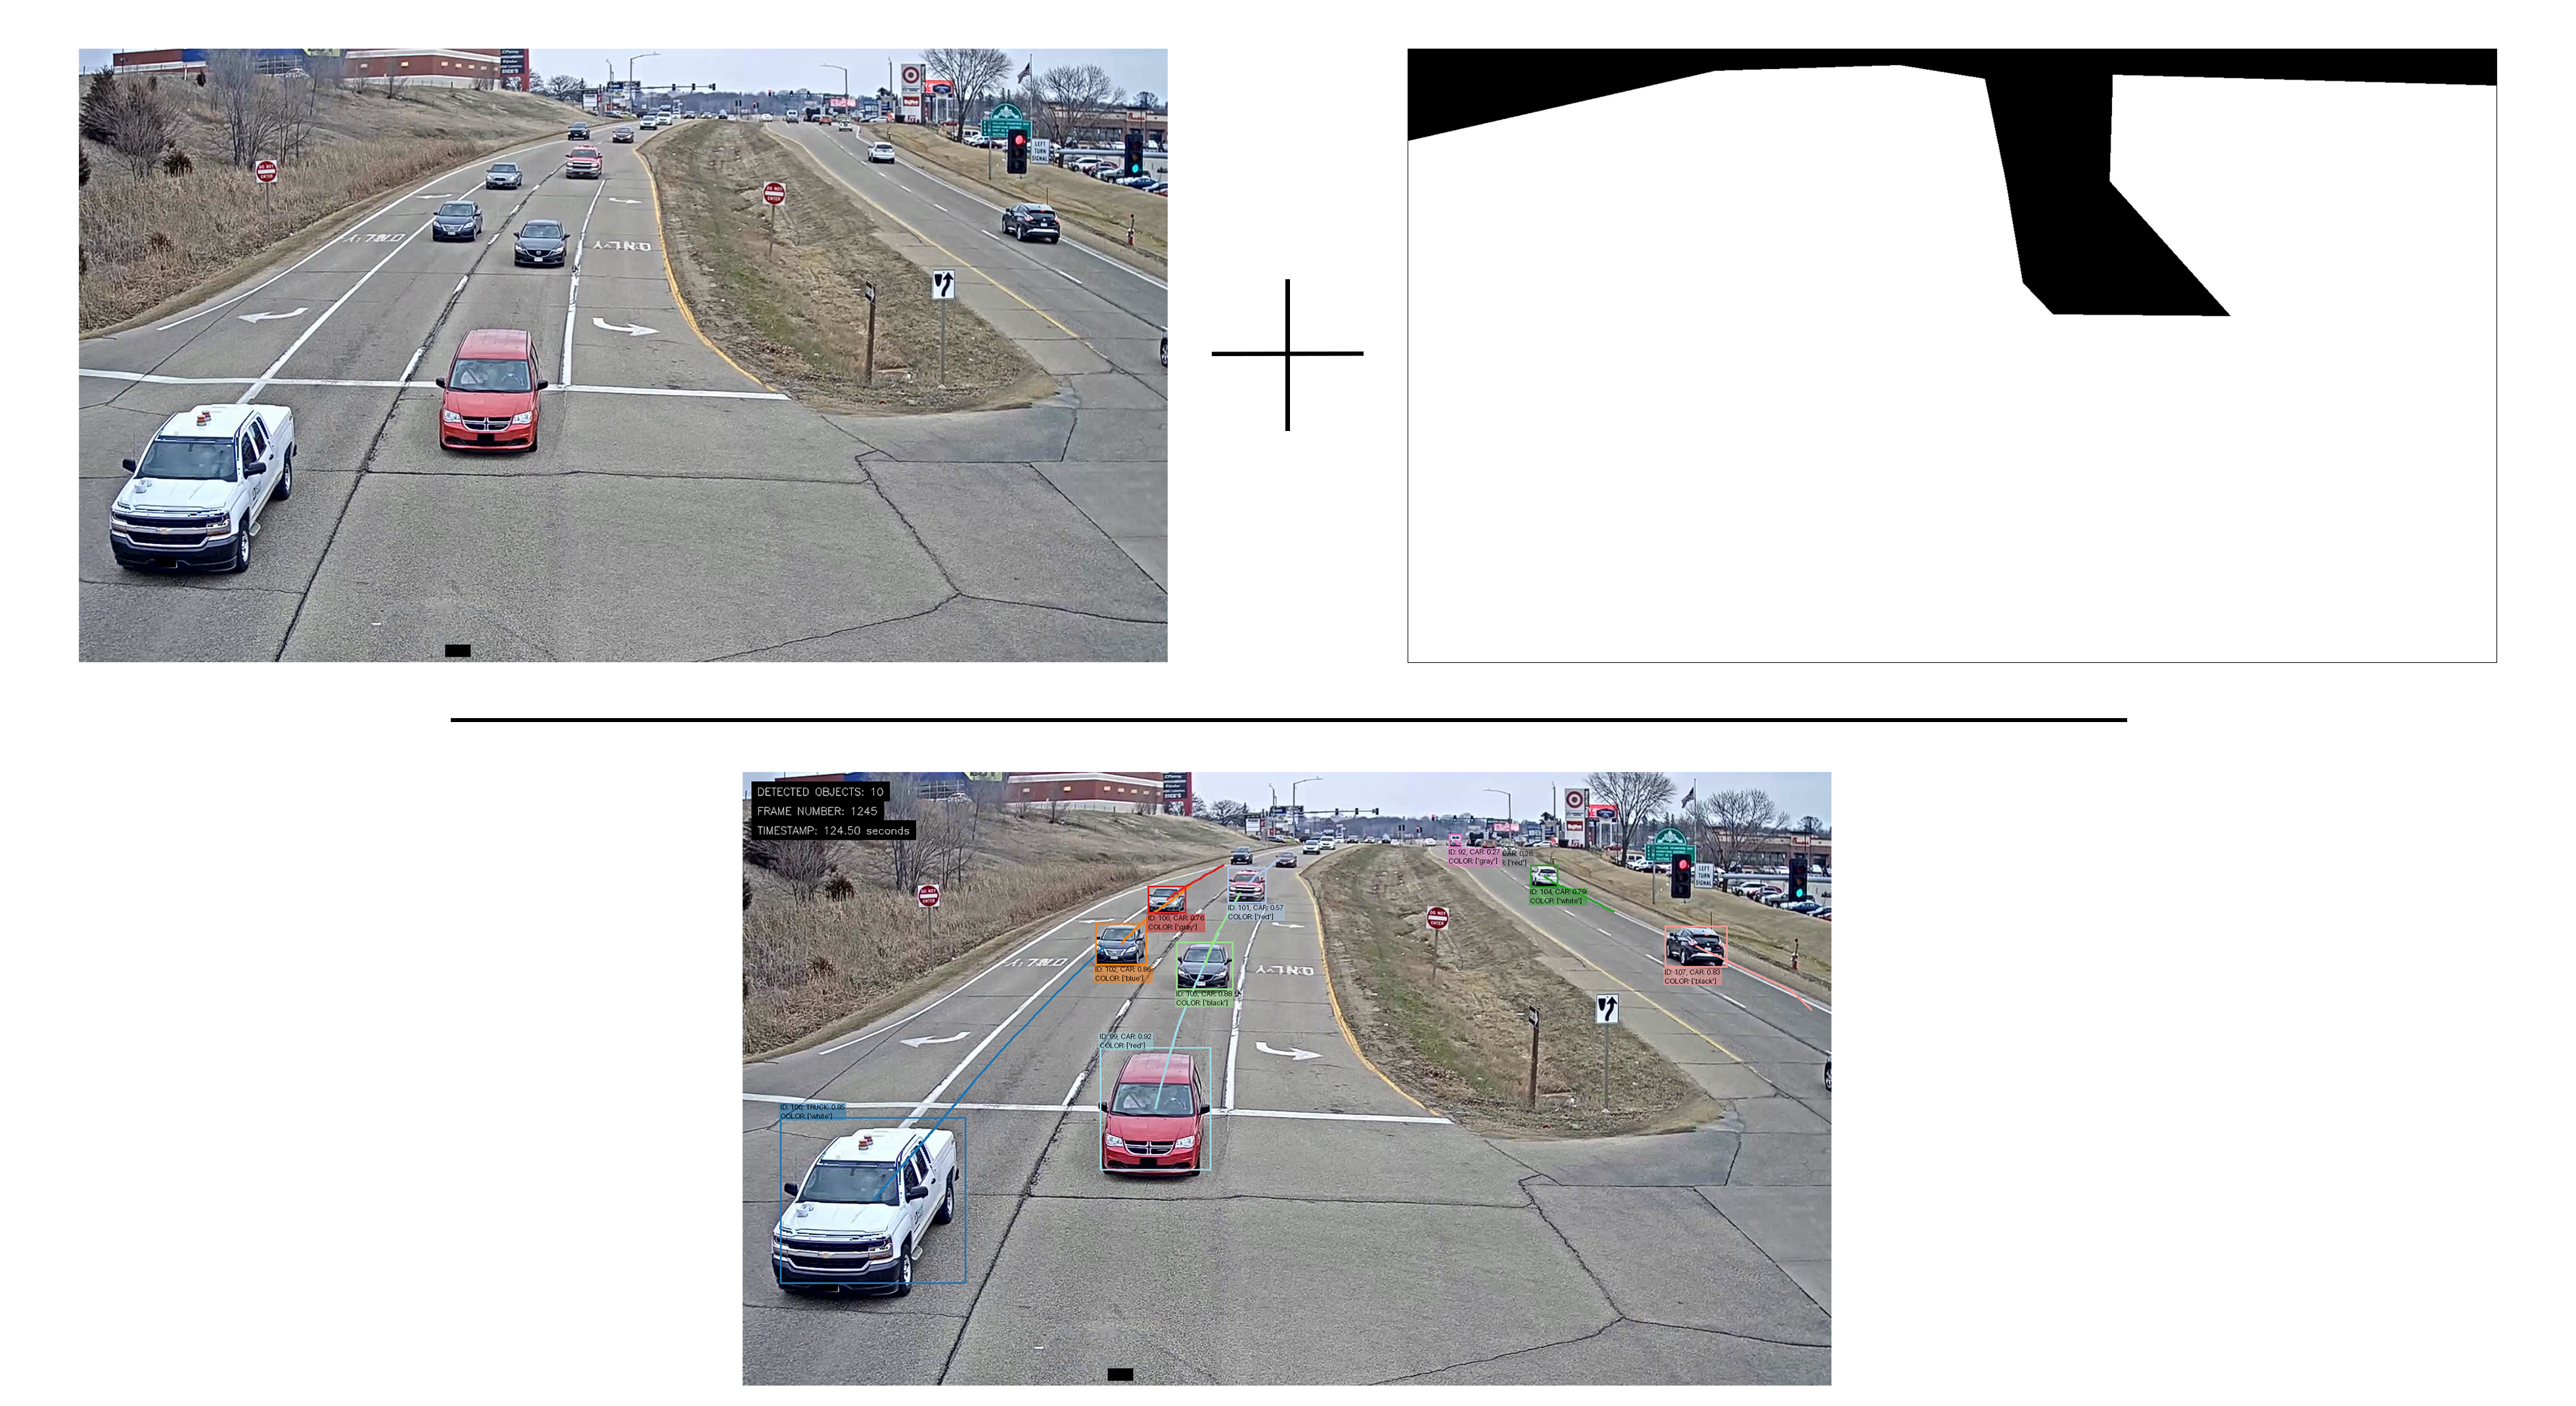
\includegraphics[width=1.0\textwidth]{images/ObjDetectionTracking.png}
    \caption[Object Detection and Tracking example]{Object Detection and Tracking example. The ROI is the area where vehicles are expected to appear.}
    \label{fig:ObjDetectionTracking}
\end{figure}

The bounding box are converted from the YOLO format (XYWH) to the MOT format (TLWH), which is a standard format used in multi-object tracking datasets, consisting in a list of frame numbers, unique ID, bounding boxes coordinates and other not-so important informations like confidence score. Each vehicle information gets saved in a Python dictionary, which is then appended to a list of dictionaries, representing the vehicles in the scene.

\subsection{Filtering}
\label{subsec:Filtering}
Various filters can be enabled and applied throughout the pipeline in order to enhance data quality, rejecting unwanted data for better detection and tracking accuracy. Filters are applied throughout the pipeline, according to the user's requirements. In practice, usually those filters are activated only when the user is running the pipeline in \textit{Target Mode} and not when evaluating the MTMC phase on the AICity Dataset (\textit{Evaluate Mode}). The following filters are available:

\subsubsection{Stationary vehicle filtering}
The stationary vehicle filter is used to filter vehicles based on their stationary status, improving the quality of the re-identification process and eliminating irrelevant vehicles. This filter is useful in scenarios where the vehicle is parked and remain static for a prolonged period of time, a condition where the tracker will always keep track of it, thus not contributing to a proper multi-camera re-identification process.

The stationary filtering algorithm works by analyzing the movement of the centroid of a vehicle's bounding box across consecutive frames. Let $(x_{t}, y_{t})$ be the centroid of the bounding box at time $t$, and $(x_{t-1}, y_{t-1})$ be the centroid at time $t-1$. The centroids are calculated simply as:
\[
    x_t = tx_t + \frac{w_t}{2}, \quad y_t = ty_t + \frac{h_t}{2}
\]

where \(tx_t\) and \(ty_t\) are the top-left coordinates of the bounding box, and \(w_t\) and \(h_t\) are its width and height, respectively.

Next, the algorithm calculates the frame-to-frame shift of the centroid by computing absolute differences of the \(x\)- and \(y\)-coordinates:

\[
    \Delta x_t = |x_t - x_{t-1}|, \quad \Delta y_t = |y_t - y_{t-1}|
\]

A frame is considered stationary if the movement in both directions is below a predefined threshold \(\tau\) relative to the frame dimensions \(W\) and \(H\):

\[
    \Delta x_t \leq \tau \cdot W, \quad \Delta y_t \leq \tau \cdot H
\]

The algorithm then counts the number of frames in which the vehicle remains stationary. If the total number of such frames exceeds a specified minimum threshold \(M\), the vehicle is classified as stationary and removed from the dataset:

\[
    \verb|stationary_frame_count| > M \implies \verb|remove_vehicle(ID)|
\]

This will filter out the vehicles which are either stationary or running very slowly, which are irrelevant for re-identification across multiple cameras. The two most important parameters here are the stationary threshold \( \tau \) and minimum stationary frame count \( M \), that are tuned to make a good trade-off between the sensitivity of the filter and the error of removing slowly moving vehicles. An example is illustrated in Figure \ref{fig:StationaryFiltering}.

% Stationary Filtering Image
\begin{figure}[H]
    \centering
    \includegraphics[width=1.0\textwidth]{images/StationaryFiltering.png}
    \caption[Stationary Filtering]{Stationary Vehicle Filtering example. $t$ denotes the current processed frame.}
    \label{fig:StationaryFiltering}
\end{figure}

\subsubsection{Incomplete Bounding Box Filtering}
To further enhance the robustness of the re-identification process, incomplete or improperly detected bounding boxes are filtered out. These bounding boxes often arise from occlusions, partial visibility of vehicles, or errors in the object detection stage. Removing such incomplete bounding boxes ensures that only high-quality data is passed to subsequent stages.

The filtering procedure starts by iterating over the set of detected frames and determining whether a bounding box should be considered incomplete based on several geometric constraints. Let \((tx, ty, w, h)\) denote the top-left coordinates, width, and height of a bounding box in a frame of dimensions \((W, H)\). The criteria used for determining incompleteness are as follows:

\paragraph{1. Minimum Size Check}
A bounding box is considered incomplete if its width or height falls below a predefined minimum size threshold \(s_{\text{min}}\):

\[
w < s_{\text{min}} \quad \text{or} \quad h < s_{\text{min}}
\]

\paragraph{2. Boundary Check}
To avoid including bounding boxes that extend beyond the visible frame area, a margin \(m\) is defined, and the bounding box is considered incomplete if any part of it lies outside the valid region:

\[
tx < m \quad \text{or} \quad ty < m \quad \text{or} \quad tx + w > (W - m) \quad \text{or} \quad ty + h > (H - m)
\]

\paragraph{3. Central Region Check}
Bounding boxes are expected to be located within a central region of the frame, defined by a central threshold \(\tau_{\text{center}}\). The bounding box centroid \((cx, cy)\) is calculated as follows:

\[
cx = tx + \frac{w}{2}, \quad cy = ty + \frac{h}{2}
\]

The bounding box is considered incomplete if its centroid lies outside the central region defined by the limits:

\[
\frac{\tau_{\text{center}}}{2} \cdot W < cx < \left(1 - \frac{\tau_{\text{center}}}{2}\right) \cdot W, \quad \frac{\tau_{\text{center}}}{2} \cdot H < cy < \left(1 - \frac{\tau_{\text{center}}}{2}\right) \cdot H
\]

After applying the above checks, frames containing incomplete bounding boxes are filtered out. The algorithm then computes the number of frames removed during this process, which is given by the difference between the initial and final frame counts. The filtering procedure ensures that only well-detected and complete bounding boxes are retained, thereby improving the reliability of subsequent multi-camera re-identification stages. A visual representation of the Incomplete Bounding Box Filtering is shown in Figure \ref{fig:IncompleteBBFiltering}.

% Incomplete Bounding Box Filtering Image
\begin{figure}[H]
    \centering
    \includegraphics[width=1.0\textwidth]{images/IncompleteFiltering.png}
    \caption[Incomplete Bounding Box Filtering]{Illustration of the incomplete bounding box filtering process. The red and green bar at the top represents frame evaluation: green segments indicate frames with complete bounding boxes that are retained, while red segments indicate frames discarded due to incomplete bounding boxes. Below, bounding boxes are shown around detected vehicles, highlighting which frames passed or failed the completeness check.}
    \label{fig:IncompleteBBFiltering}
\end{figure}

\subsubsection{Color Filtering}
\label{subsubsec:ColorFiltering}
If there are still more frames to process, a color filter can be applied to further refine the dataset. This particular filter eliminates any vehicles not matching an predefined set of target colors. This filter comes in handy in situations when the color of the vehicle is known and the user wants to track only those vehicles of that specific color. This restriction improves the general quality of the Re-ID results, mostly when the process is running, again, in \textit{Target Mode}.

The algorithm starts by checking if the list of target colors $\mathcal{C}_{\text{target}}$ is empty. If no target colors are defined, then the function will terminate early and return the original list of frames. Otherwise, it proceeds with the filtering process based on the color predictions.

Considering a set of frames \(\mathcal{F} = \{f_1, f_2, \ldots, f_N\}\) that corresponds to a specific vehicle identification number, the algorithm further continues to pull the cropped images \(\mathcal{I} = \{I_1, I_2, \ldots, I_N\}\) which depict the detected vehicle in each corresponding frame.

For every image \(I_i \in \mathcal{I}\), the following operations are carried out:
\begin{enumerate}
    \item The image \(I_i\) is converted from an array type to a PIL image.
    \item A transformation function \(T_{\text{val}}\) is applied to prepare the image for inference. This includes resizing, normalization, and conversion to a tensor.
    \item The preprocessed image is then passed through the color classification model.
\end{enumerate}

The color classification model, denoted as $f_{\text{Color}}$, can be one of the following:
\begin{itemize}
    \item A model based on \textbf{EfficientNet} architectures (B3 or B5 variants) where predictions are directly produced as a sequential list of color labels:
    \[
        \text{color\_prediction} = f_{\text{Color}}(I_{i})
    \]
    \item A \textbf{ResNet} architecture integrated with a \textbf{Support Vector Machine} (SVM) classifier. Initially, feature embeddings are obtained via the Re-ID model \(f_{\text{ReID}}\), after which the SVM classifier tries to predict the color:
    \[
        f_{emb} = f_{\text{ReID}}(I_i), \quad \verb|color_prediction| = f_{\text{Color}}(f_{emb})
    \]
\end{itemize}

Regarding the training component for both models, a Multi-Dataset approach combining \textit{VeRi-776} and \textit{VeRi-Wild} datasets has been implemented. The main problem regarding this strategy was the lack of data, hence the creation of a Unified Dataset which combines multiple images and labels from the training set of both datasets. In fact, the unified color classification system harmonizes and deduplicates color labels across both datasets, ensuring consistent color identification across different instances of vehicle datasets. For this matter, a total of 10 color classes were defined, including the most common vehicle colors such as white, black, silver, blue, red, etc. using a total of 300k images were used for training. Another peculiarity of the training process is the choice of the Dataset size. For this reason, the user had the free choice to select the size of the dataset to be used for training, which could range between 1\% and 100\% of the total dataset size. This choice was made to allow the user to train the model with a smaller dataset, which could be useful in case of limited computational resources or time constraints.

The configuration framework employs several key parameters and optimization strategies as the ones followed by the Feature Extraction protocol. Image preprocessing and augmentation strategies were carefully considered. All images undergo standardization to $320 \times 320$ pixels, while maintaining aspect ratios through centered padding rather than aggressive cropping or stretching. The augmentation pipeline includes random horizontal flipping with 0.5 probability as well. Notably, color-based augmentation techniques such as jitter, contrast, and saturation adjustments were intentionally disabled to preserve color fidelity for the classification task.
The training methodology implements a comprehensive loop encompassing both training and validation phases. The loss function utilizes CrossEntropyLoss for classification tasks, while the Adam optimizer handles parameter updates. A particularly significant aspect of the implementation is the sophisticated handling of varying image dimensions. Rather than employing traditional resizing methods that might distort aspect ratios, the system implements a centered padding approach. This methodology preserves the original image proportions while ensuring consistent batch processing capabilities.

Continuing with the filter stage, if the predicted color does not match any of the target colors, the frame is marked for removal, resulting in a final filtered set of frames \(\mathcal{F}_{\text{filtered}}\) for the vehicle ID. The algorithm then calculates the number of frames eliminated during this step by subtracting the original and final number of frames. Color filtering helps the algorithm keep only those vehicles who do match the target colors list, previously defined, thus making the re-identification process of much better quality. An example of the Color Filtering process is depicted in Figure \ref{fig:ColorFiltering}.

% Color Filtering Image
\begin{figure}[H]
    \centering
    \includegraphics[width=1.0\textwidth]{images/ColorFiltering.png}
    \caption[Color Filtering]{If \(\mathcal{C}_{\text{target}} = ['blue']\), only the right truck, with \(ID = 20\), will be taken into consideration when computing the final re-identification results.}
    \label{fig:ColorFiltering}
\end{figure}

\subsubsection{Minimum frame detection}
Minimum frame detection is a filter that will further refine the frames. The filter can remove those vehicles which are detected for very short durations probably because of false positives or for transient objects. A filter like this will validate only those vehicles which get detected for a number of frames equal or higher than a predefined minimum, hence enhancing the quality in re-identification. It also sets, for every vehicle ID, a global class label, which corresponds to the most frequent class label that the pipeline assigns during the Object Detection phase - avoiding the common little interchanging of class labels between consequent frames.

\subsection{Feature Extraction}
Feature extraction involves the Re-ID model, which will extract the features from the saved frames. The inputs would be the cropped images of the vehicles and, after the inference, a feature vector for each vehicle will be given as output. Actually, the whole methodology followed is very similar to that which has been followed for the color filtering procedure. Feature extraction becomes very important when it comes to the re-identification task since the previously extracted features would then form a basis of comparison for vehicle similarity in diverse cameras, even though that is out of the scope for this subsection.

\subsection{Trajectory Creation}
The trajectory creation process will create a separate trajectory record for each vehicle detected over frames, by properly storing it in a MongoDB database or Pickle files. This step is essential in the Multi-Target Multi-Camera (MTMC) tracking task, as it helps in linking vehicle detections temporally as well as across different camera perspectives.

For every detected vehicle ID, the following steps are performed:

\begin{enumerate}
    \item A \textbf{unique Vehicle ID} is obtained by appending the camera ID with the vehicle ID. It gives an identifier of the form:
    \[
        VehicleID = CAM_{i}\_V_{j}  \quad \text{(e.g., CAM0\_V10)}
    \]
    where \(i\) and \(j\) represent are the camera ID and vehicle ID, respectively.
    \item A corresponding \textbf{Trajectory ID} is created by appending a suffix to the unique vehicle ID:
    \[
        TrajectoryID = CAM_{i}\_V_{j}\_T_{k}  \quad \text{(e.g., CAM0\_V10\_T0)}
    \]
    where \(i, j, k\) represent the Camera ID, Vehicle ID, and Trajectory Index, respectively.
    
    \item Each frame in the sequence undergoes the following processing steps:
    \begin{itemize}
        \item Compression of the cropped vehicle image using an appropriate compression method (\textit{byte-level compression}) in order to save it in MongoDB in an efficient way.
        \item Extraction of the bounding box shape and feature vectors list conversion for efficiency.
        \item Generation of a \textbf{unique bounding box ID} for every frame by appending the frame index as well:
        \[
            BBoxID = CAM_{i}\_V_{j}\_F_{b} \quad \text{(e.g., CAM0\_V10\_F0)}
        \]
        where \(i, j, b\) denotes the camera ID, vehicle ID, and frame index, respectively.
    \end{itemize}

    \item The \textbf{start and end times} of the trajectory are determined from the timestamps of the first and last frames in the sequence.
\end{enumerate}

After the trajectory creation process is done, data is inserted in the MongoDB database. The insertion process consists of the following:

\begin{enumerate}
    \item \textbf{Vehicle Insertion:} Before inserting a new vehicle record, the database is queried to check whether the vehicle already exists. If the vehicle does not exist, a new record is created with its unique ID and class label. The vehicle record is composed by: Vehicle ID and Class Label.
    
    \item \textbf{Bounding Box Insertion:} In every frame, a bounding box record is inserted into the database. If a bounding box with the same ID already exists, the record is updated by incrementing the frame index. The vehicle record is composed by: Frame Index, Bounding Box ID, Bounding Box Shape, Vehicle ID, Compressed Image, Confidence Score, Feature Vector and Timestamp.
    
    \item \textbf{Trajectory Insertion:} The trajectory record, containing the unique trajectory ID, vehicle ID, camera ID, start and end times, is inserted into the database. If the trajectory already exists, it is updated with additional frames. The trajectory record is composed by: Trajectory ID, Vehicle ID, Camera ID, Start Time, End Time.
\end{enumerate}
    
This process, therefore, ensures that the system can handle vehicle tracking in real-time without losing data integrity and by the minimization of redundant entries.

\subsection{Unification}
\label{subsec:Unification}

The unification step tries to enhance the output of the Re-ID pipeline by unifying the set of different vehicle identities that might have been assigned different IDs despite referring to the same physical vehicle. This step is very important in increasing the coherence and accuracy of Multi-Object Tracking and Re-Identification in a single-camera setting. This is precisely shown in Figure \ref{fig:Unification}.

% Unification Image
\begin{figure}[H]
    \centering
    \includegraphics[width=0.90\textwidth]{images/IDSwitch.png}
    \caption[An ID-Switch example]{Unification process. Cars with ID 60 and 59 (top image, left corner) get a mis-assigned ID after the truck with ID 64 passes, as shown in the bottom figure. The unification process aims to merge these IDs into a single one.}
    \label{fig:Unification}
\end{figure}

Once the initial steps in the pipeline - namely, detection and tracking - have been completed, the unification algorithm starts to compute pairwise similarities of features between the vehicles detected by the same camera. Towards this end, an accurate hand-crafted function is adopted that identifies pairs of vehicle IDs with top similarity scores according to multiple unification techniques.
\begin{itemize}
    \item \textbf{Mean Embedding Comparison}: For every vehicle \( v_i \) captured by a camera, the mean embedding is calculated by averaging the feature vectors of all frames associated with that vehicle. Let \( \mathbf{f}_{i}^{(t)} \in \mathbb{R}^{d} \) denote the feature vector of vehicle \( v_i \) at time \( t \), where \( d \) is the dimensionality of the embedding space. The average embedding \( \bar{\mathbf{f}}_{i} \) corresponding to the vehicle \( v_i \) can be expressed as:
    \[
        \bar{\mathbf{f}}_{i} = \frac{1}{T_i} \sum_{t=1}^{T_i} \mathbf{f}_{i}^{(t)}
    \]
    where \( T_i \) denotes the cumulative count of frames in which the vehicle \( v_i \) is present.
    The computation of pairwise similarity \( S(i, j) \) between two vehicles \( v_i \) and \( v_j \) is conducted through the application of cosine similarity, expressed mathematically as follows:
    \[
        S(i, j) = \frac{\bar{\mathbf{f}}_{i} \cdot \bar{\mathbf{f}}_{j}}{\|\bar{\mathbf{f}}_{i}\| \|\bar{\mathbf{f}}_{j}\|}
    \]
    \item \textbf{Individual Frame Comparison}: The similarity of two vehicles is determined by comparing the feature vectors corresponding to their frames individually and then computing the average of the obtained similarities. Let $\mathcal{F}_i$ and $\mathcal{F}_j$ be the sets of feature vectors for vehicles $v_i$ and $v_j$, respectively. The similarity measure $S(i, j)$ between the two vehicles is defined as:
    \[
        S(i, j) = \frac{1}{|\mathcal{F}_i| \cdot |\mathcal{F}_j|} \sum_{\mathbf{f}_p \in \mathcal{F}_i} \sum_{\mathbf{f}_q \in \mathcal{F}_j} \frac{\mathbf{f}_p \cdot \mathbf{f}_q}{\|\mathbf{f}_p\| \|\mathbf{f}_q\|}
    \]
    where $\mid\mathcal{F}_i\mid$ and $\mid\mathcal{F}_j\mid$ denote the number of frames in which vehicles $v_i$ and $v_j$ respectively appear. Such a measure allows finer comparison by examining the similarity of individual frames; it also has the drawback that the computation might take longer since more comparisons need to be done, hence, not suitable for real-time operations.
    \item \textbf{Comparison of Area-Weighted Embeddings}: In this context, each feature vector is assigned a weight that corresponds to the relative area of its associated bounding box. The weight \( w_{i}^{(t)} \) for vehicle \( v_i \) at a given time \( t \) is expressed as follows:
    \[
        w_{i}^{(t)} = \frac{A_{i}^{(t)}}{\min\limits_{t} A_{i}^{(t)}}
    \]
    Here, \( A_{i}^{(t)} \) denotes the bounding box area at time \( t \), which can be formulated as:
    \[
        A_{i}^{(t)} = w_{i}^{(t)} \times h_{i}^{(t)},
    \]
    and \( \min_{t} A_{i}^{(t)} \) denotes the minimum bounding box area across all frames for vehicle \( v_i \).
    The area-weighted average embedding \(\ bar{\mathbf{f}}_{i} \) for the vehicle \( v_i \) is obtained via the following formula:
    \[
        \bar{\mathbf{f}}_{i} = \frac{\sum_{t=1}^{T_i} w_{i}^{(t)} \mathbf{f}_{i}^{(t)}}{\sum_{t=1}^{T_i} w_{i}^{(t)}}
    \]
    Finally, the pairwise similarity \( S(i, j) \) between vehicles \( v_i \) and \( v_j \) is computed using the cosine similarity of their area-weighted mean embeddings:
    \[
        S(i, j) = \frac{\bar{\mathbf{f}}_{i} \cdot \bar{\mathbf{f}}_{j}}{\|\bar{\mathbf{f}}_{i}\| \|\bar{\mathbf{f}}_{j}\|}
    \]
\end{itemize}

After finding the most alike pairs of vehicles, the merging process begins. For each pair $(ID_i, ID_j)$ whose similarity score exceeds a predefined threshold, spatial-temporal constraints are applied:
\begin{itemize}
    \item \textbf{Time Gap Threshold}: The time gap between the last observation of $ID_i$ and the first observation of $ID_j$ has to be less than a predefined maximum threshold.
    \item \textbf{Spatial Distance Threshold}: The Euclidean distance calculated between the centroids of the final bounding box corresponding to $ID_i$ and the initial bounding box associated with $ID_j$ has to be below a predefined range.
\end{itemize}

If both conditions are satisfied, the two tracklets are merged by updating the database entries. In detail, the bounding boxes and the trajectory information belonging to $ID_j$ are assigned to $ID_i$, with $ID_j$ being removed from the database. In addition, if the bounding box images are saved to the local disk (through a specific configuration parameter), the corresponding image files are moved to the folder of $ID_i$.

The unification process can enhance the reliability of the system because it unifies those fragmented tracklets, related to the same vehicle, into a single and coherent identity. It also diminishes the prevalence of redundant identities in a single camera, enhancing its overall Re-ID performance.

\subsubsection{Final Data Export and Storage}
Once all the frames have been processed and the necessary information has been extracted, the final action involves storing the results in a \texttt{.txt} file in a MOTChallenge compliant format.

It all starts by collecting data from the database and by fetching all frames corresponding to a given camera ID. For each vehicle ID, it extracts the frame-level properties, including feature vectors, compressed images, bounding box coordinates, timestamps, and confidence scores. Let \( \mathcal{F} \) be the set of frames of a vehicle \( v \) captured by camera \( c \), where each frame \( f \in \mathcal{F} \) has the following information:
\[
    f = (\mathbf{e}, \mathcal{I}_{\text{comp}}, s, n, b, t, \alpha, v)
\]
where:
\begin{itemize}
    \item \( \mathbf{e} \) represents the feature vector,
    \item \( \mathcal{I}_{\text{compressed}} \) denotes the compressed image data,
    \item \( s \) is the shape of the frame,
    \item \( n \) is the frame number,
    \item \( b = (x, y, w, h) \) defines the bounding box in Top-Left Width-Height (\textit{TLWH}) format,
    \item \( t \) is the timestamp,
    \item \( \alpha \) is the confidence score,
    \item \( v \) is the vehicle ID.
\end{itemize}

For each bounding box, the top-left coordinates \((x, y)\), along with width \(w\) and height \(h\) are extracted and written into a \texttt{.csv} file following the MOTChallenge format:
\[
    \text{Row} = (\text{FrameID}, \text{TrackID}, x, y, w, h, \text{Confidence}, X_{\text{world}}, Y_{\text{world}}, Z_{\text{world}})
\]
The confidence score is set to 1 and real-world coordinates \( (X_{\text{world}}, Y_{\text{world}}, Z_{\text{world}}) \) are initialized to -1, as they are not used in this specific pipeline.
These storage paths are generated dynamically based on the camera ID and a predefined global path for proper organization and retrieval of results at different test scenarios.

\subsection{MTMC and Final Clustering Stage}
\label{subsec:MTMC}

The last part of the pipeline includes steps for \textbf{Multi-Target Multi-Camera (MTMC) tracking} and clustering in order to connect trajectories across multiple cameras. The stage allows to unify the tracks of the same vehicle seen by cameras at different views to a coherent single trajectory.

\subsubsection{Cross-Camera Analysis Setup}
The process begins by loading the \textit{Camera Layout}, which contains spatial and temporal information about the cameras, including their locations and their relative mutual compatibility. The system ensures that vehicles appearing in compatible cameras, meaning cameras which have overlapping FOVs and with overallping time intervals, can be considered for linking.

Some key cross-camera spatial and temporal calibrations will be pursued with the help of the \textit{Camera Layout} itself. Some major parameters are shown as follows:
\begin{itemize}
    \item \textbf{FPS (Frames per Second)}: Frame rate of the cameras.
    \item \textbf{Scales}: An array of multiplicative factors which is used for normalizing the time values across the different cameras.
    \item \textbf{Offsets}: Temporal offsets to bring cameras to a common and synchronized starting time.
    \item \textbf{Compatibility Matrix}: A binary matrix indicating whether two cameras have overlapping fields of view, hence they are compatible.
    \item \textbf{Transition Windows} (\(\text{dt}_{\min}\) and \(\text{dt}_{\max}\)): Minimum and maximum time intervals allowed for a vehicle to transition between cameras.
\end{itemize}

The \textbf{scales} and \textbf{offsets} parameters serve to adjust small temporal differences between cameras when linking tracklets. As different cameras may have slight variations in recording speed or starting times, these parameters align events properly across the multi-camera setup.
The scale for a given camera \(i\) is computed as:
\[
    \text{scale}_i = \frac{t_{2}}{t_{1}}
\]
where \(t_{1}\) and \(t_{2}\) are the times taken for the same event to occur on the reference camera and camera \(i\), respectively.

Similarly, the offset for a camera \(i\) is given by:
\[
    \text{offset}_i = t_{1} - t_{2}
\]
where \(t_{1}\) and \(t_{2}\) are the appearance times of the same vehicle in the beginning of the video on the reference camera and camera \(i\), respectively.

The vehicle tracklets are collected either from a precomputed \textit{Pickle} file or directly from the database, depending on the configuration. Each tracklet includes frames, bounding boxes, timestamps, and extracted features.

\subsubsection{Tracklet Construction}
For each camera, tracklets are constructed using the collected frames from the DB or the Pickle files.
Each tracklet will include:
\begin{itemize}
    \item \textbf{Vehicle ID}, which indicates the unique ID of the vehicle.
    \item \textbf{Mean Feature}, computed as the average of the frame features. Necessary for globally representing the tracklet.
    \item \textbf{Start and End Times}, derived from the timestamps of the first and last frames. More precisely, Camera parameters come into play, since the $\textit{global}$ start and end times of each tracklet is being computed. For a tracklet \( \text{track} \) in camera \(i\) with local start time \(t_{\text{start}}\) and end time \(t_{\text{end}}\), the global times are computed as:
    \[
    T_{\text{start}} = \frac{t_{\text{start}}}{\text{fps}_i \cdot \text{scale}_i} + \text{offset}_i
    \]
    \[
    T_{\text{end}} = \frac{t_{\text{end}}}{\text{fps}_i \cdot \text{scale}_i} + \text{offset}_i
    \]
\end{itemize}
This information is very important for the successive clustering and merging process.

\subsubsection{Similarity Matrix Computation}
The similarities between all tracklets are computed based on their mean features. For two tracklets $\text{track}_1$ and $\text{track}_2$ with their respective mean features $\mathbf{f}_1$ and $\mathbf{f}_2$, the similarity score $s$ is computed as the dot product:
\[
s = 
\begin{cases}
\mathbf{f}_1 \cdot \mathbf{f}_2, & \text{if already normalized} \\
\frac{\mathbf{f}_1 \cdot \mathbf{f}_2}{\|\mathbf{f}_1\|_2 \|\mathbf{f}_2\|_2}, & \text{otherwise}
\end{cases}
\]
When a different \textbf{linkage} method is given (such as \textit{average}, \textit{single}, or \textit{complete}), the similarity is computed by retrieving pairwise similarities from a precomputed similarity matrix \( \mathbf{S} \):
\[
    \textbf{average: } s = \frac{1}{|T_1| \cdot |T_2|} \sum_{t_1 \in T_1, t_2 \in T_2} S[t_1, t_2]
\]
\[
    \textbf{single: } s = \max_{t_1 \in T_1, t_2 \in T_2} S[t_1, t_2]
\]
\[
    \textbf{complete: } s = \min_{t_1 \in T_1, t_2 \in T_2} S[t_1, t_2]
\]

\subsubsection{Track Merging}
The two conditions below must be satisfied to merge the tracklets:
\begin{itemize}
    \item \textbf{Compatibility}: The tracklets belong to physically compatible cameras separated by an overlap of time intervals. Two cameras are compatible if their time intervals intersect a boundary condition, like:
    
    Compatible if:
    \[ T_{2, \text{start}} \leq T_{1, \text{end}} + \delta_{t_{\max}} \quad \text{and} \quad T_{2, \text{end}} \geq T_{1, \text{end}} + \delta_{t_{\min}} \]
    or viceversa:
    \[ T_{1, \text{start}} \leq T_{2, \text{end}} + \delta_{t_{\max}} \quad \text{and} \quad T_{1, \text{end}} \geq T_{2, \text{end}} + \delta_{t_{\min}} \]
    where \( \delta_{t_{\min}} \) and \( \delta_{t_{\max}} \) are the minimum and maximum time intervals allowed for a vehicle to transition between cameras.
    \item \textbf{Similarity}: The tracklets must have a similarity score greater than a threshold (\( \theta_{\text{sim}} \)).
\end{itemize}

\subsubsection{A Priority Queue for Track Merging}
A \textbf{priority queue} is utilized to manage merging tracklets across cameras. This priority queue contains candidate pairs of tracklets to be merged sorted in descending order by their similarity scores. Each entry in the queue will be represented as:
\[
    \text{Entry} = (-\text{similarity}, \text{timestamp}, \text{track}_i, \text{track}_j)
\]
here, negative similarity implements a \textit{max-heap}, so pairs with highest similarity will be first processed.

The similarity between two tracklets is computed as the dot product between their normalized mean feature vectors:
\[
    \text{similarity}(\text{track}_i, \text{track}_j) = \frac{\mathbf{f}_i \cdot \mathbf{f}_j}{\|\mathbf{f}_i\|_2 \|\mathbf{f}_j\|_2}
\]
where \(\mathbf{f}_i\) and \(\mathbf{f}_j\) denote the mean feature vectors of the two tracklets.

To speed up the computation of similarity, all mean features are stacked into a matrix \(\mathbf{F}\), and the similarity matrix is computed by a matrix multiplication:
\[
    \mathbf{S} = \mathbf{F} \cdot \mathbf{F}^\top
\]

This technique exploits GPU acceleration with \texttt{torch}, thus reducing the time complexity relative to pairwise dot products. Next, once the similarity matrix has been computed, there is a collection of tracklets, which are appended to the priority queue for further merging based on the similarity score above a given threshold.

During merging, if a pair of tracklets are spatially and temporally compatible, they will be merged and the similarity matrix is updated. The above procedure proceeds until there are no more compatible pairs in the priority queue. In other words, the pipeline itself performs an incremental merging of tracklets depending on their visual similarities but certainly also taking into consideration motion constraints.

\subsubsection{Final Prediction Output}
Once the merging process is complete, the final consolidated trajectory will thus be saved in the \textbf{MOTChallenge format}. For each camera, the system then generates a prediction file containing:
\begin{itemize}
    \item Frame number
    \item Track ID
    \item Bounding box coordinates (in \textit{TLWH} format)
    \item Confidence score
\end{itemize}
A \textit{Pickle} file is also generated containing the final tracklets with their corresponding frames and features for further analysis.

\subsection{Target Mode}
The pipeline, as previously teased, can operate in \textit{Target Mode}, which means that the user would like to track a particular vehicle of interest in a series of various camera views. In this specific operating mode, the pipeline will not compute the MTMC metrics corresponding to the AICity Dataset; instead, it takes as input a reference picture of the target vehicle and a corresponding camera ID which specifies from which the picture has been taken. The system, therefore, utilizes the same Deep Learning-based Re-ID features used in the MTMC clustering step to find the most similar vehicle instances across the entire camera network immediately after the MTMC pipeline has successfully been executed (i.e., meaning just after the Trajectory Creation step and the Final Clustering phase).

The target vehicle identification can be done by one of the following three ways:

\begin{itemize}
    \item \textbf{Multi-track Search}: This method is first performed aggregating the vehicle detections into a complete trajectory and then comparing the target vehicle with the average feature embeddings of each trajectory. With the intent of thereby avoiding false positives, it specifically excludes any trajectory starting from the same camera as the target vehicle and, in particular, focuses on the inter-camera matches. The similarity is then computed using normalized feature vectors which returns the top-K most similar trajectories. Overall, this method employs the MTMC final clustering trajectories to access the most comparable occurrences of the target vehicle across different cameras.
    \item \textbf{Single-track Search}: This is even more accurate and detailed as it provides better comparisons of the target vehicle against single vehicle tracks rather than whole trajectories. It can be used effectively in cases of partial or fragmented trajectories because it assesses each track individually without requiring a complete trajectory reconstruction. Again, just like the others, trajectories from the same camera are also excluded. 
    \item \textbf{Camera-link Search}: The most advanced method is to construct trajectories incrementally between cameras. It will start with finding the optimal matches in the first camera, and from there it will progressively connect to the next most similar vehicle in the following cameras. This method performs best in consistent identity across the entire camera network since it uses spatial links among the cameras.
    All three methods are based on the same Re-ID model which produce stable and reliable features for the target vehicle.
    The feature extraction for the Target Vehicle is similar to the others, while the similarity is calculated through the same cosine similarity measure. The system generates a ranked list of potential matches, which allows the user to view the most probable examples of the target vehicle from different camera views. This feature is of special value in applications like law enforcement, traffic monitoring, or analysis of vehicle movement patterns in an urban environment. An example is shown in Figure \ref{fig:TargetSearch}.
\end{itemize}

% Target Mode Image
\begin{figure}[H]
    \centering
    \includegraphics[width=1.0\textwidth]{images/TargetSearch.png}
    \caption[Target Search Results]{An example of the Target Mode search. In this example, the first row denotes the top-result coming from the pipeline. The Target Vehicle is not present in first row - Camera 1 because it passes below the camera view FOV, hence it's not present in the overall system.}
    \label{fig:TargetSearch}
\end{figure}

% Pipeline Overview Image
\begin{figure}[ht]
    \centering
    \includegraphics[width=1.0\textwidth]{images/PipelineOverview.png}
    \caption[Pipeline overview]{Pipeline Overview. The pipeline consists of several stages, including Re-ID Training, Object Detection, Tracking, Filtering, Feature Extraction, Trajectory Creation, Unification and MTMC Final Tracking. Color filtering is only applied in Target Mode.}
    \label{fig:PipelineOverview}
\end{figure}

    \clearpage
    \chapter{Experiments}
\label{chap:Experiments}

\section{Training \& MTMC Hyperparameters}
In this subsection, we present the essential configurations and hyperparameters used during the training process for the Feature Extraction model and for the MTMC (Multi-Target Multi-Camera) tracking stage. These settings directly influence the model's performance and its ability to generalize across varying scenarios. All tests have been carried on n. 2 NVIDIA Tesla A4000 GPUs with 16GB of VRAM each.

A detailed description of the network setup, datasets used for the experiments, metrics, optimizer, scheduler, and data augmentation strategies is provided to offer insights into the experimental framework.

\subsection{Network setup}
As for the Feature Extraction model, a pre-trained ResNet-IBN-50 architecture has been used as backbone. The model weights are pre-trained on ImageNet and the model itself uses the BNNeck architecture, along with setting the last stride of the Convolutional Filter, in the last block, equal to 1, as previously explicited in \ref{subsubsec:Stride} and \ref{subsec:BNNeck}.

\subsection{Loss}
The loss function used for training the Feature Extraction model is the combination of the ID Loss and the Metric Loss, as described in \ref{subsec:LossFunctions}. The ID Loss, used to classify the input images into the correct class, follows a standard Cross Entropy with the label smoothing parameter $\beta = 0.20$. As for the Metric Loss, a standard Triplet Loss is used to minimize the distance between the anchor and the positive samples, and to maximize the distance between the anchor and the negative samples. Its margin parameter $\alpha$ is set to 0.3.
As for the MALW training loop, a standard parameter search was able to set $K = 2000$ as the most favorable value, hence every 2000 iterations the $\lambda_{ID}$ parameter (ID weight) gets updated following the standard deviation of the ID Loss itself, while the $\lambda_{Metric}$ parameter (Metric Loss weight) is simply set to 1.0.

\subsection{Dataloaders}
As for the Dataloaders, we follow what has been detailed in \ref{subsubsec:DataloaderSampling}, where \textit{Random Sampling} was chosen as the sampling strategy and the parameter $K$ and $P$ are set to 36 and 6, respectively, meaning that the number of identities per batch is set to 36, while the number of images per identity is set to 6. Furthermore, the number of workers has been set equal to 8.

\subsection{Datasets}
For the proposed methodology, multiple Datasets have been used between the Feature Extraction and MultiTrack Re-Identification tasks. The Datasets, which sum up to 7, differ in terms of the number of cameras, number of vehicles and number of images as can be seen from Table \ref{table:Datasets}.

\begin{table}[ht]
    \centering
    \caption{Dataset comparisons}
    \begin{tabular}{|C{0.80in}|C{1.00in}|C{0.80in}|C{0.80in}|C{0.85in}|}
    \hline
    \textbf{Dataset} & \textbf{Purpose} & \textbf{Images} & \textbf{Vehicles} & \textbf{Cameras} \\ \hline
    \hline
    VeRi-776 & Re-ID & 49,537 & 776 & 20 \\ \hline
    VehicleID & Re-ID & 221,763 & 26,267 & Multiple viewpoints \\ \hline
    VeRi-Wild & Re-ID & 416,314 & 40,671 & 174 \\ \hline
    VRU & Re-ID & 172,137 & 15,085 & Multiple viewpoints \\ \hline
    AICity & Re-ID/MultiTrack & - & 145 & 4 \\ \hline
    \end{tabular}
    \label{table:Datasets}
\end{table}

\subsubsection{VeRi-776}
\textbf{VeRi-776} \cite{Veri776_1, Veri776_2, Veri776_3} is a Vehicle Re-ID Dataset, widely accepted as a benchmark measure, specifically designed for real-world surveillance contexts to evaluate the proposed framework for Feature Extraction. With more than \textbf{50,000} images of \textbf{776} different vehicles captured during a continuous 24-hour period in an urban area of size 1.0 km$^2$, it is one of the largest-scale and most diverse datasets with detailed annotations, making it among the most complete publicly available datasets for Vehicle Re-ID research.

It is recorded with 20 non-overlapping cameras positioned in a view to simulate realistic traffic monitoring scenarios. This setup makes it well-scalable and retains challenges relevant to practical applications of Vehicle Re-Identification. Along with that, the following characteristic features make the dataset uniquely suitable for training and evaluating the feature extraction models in complex surveillance scenarios. Specifically:

\begin{itemize}
    \item \textit{Real-world Variants}: The images are captured in unconstrained surveillance scenes, and thus, exhibit a rich set of real-world challenges such as illuminations, various resolution scales and occlusions. The vehicles are recorded from 2 to 18 different views across multiple cameras, introducing significant intra-class variability while ensuring sufficient recurrence rates, which are essential for effective cross-camera vehicle re-identification.
    \item \textit{Attribute Annotations}: The images are fully annotated with various attributes like Vehicle ID, Camera ID, Color, and Type that make it possible to train a complex Neural Network model necessary in learning complex visual features discriminating between vehicles with very subtle appearance differences.
\end{itemize}

\subsubsection{VehicleID}
The \textbf{VehicleID} \cite{VehicleID} dataset consists of a large-scale Vehicle Re-Identification dataset captured during the daytime using multiple non-overlapping surveillance cameras deployed across a small city in China. Unlike some other datasets mainly designed to target fine-grained vehicle model classification, such as the CompCars dataset \cite{CompCars}, the VehicleID dataset aims to resolve real-world tasks of vehicle retrieval and re-identification. It emphasizes representing frequently observed vehicles with consideration to the imbalanced nature that exists in real-world distribution.

This dataset contains \textbf{221,763} images of \textbf{26,267} vehicles, at an average of \textit{8.44} images per vehicle. Each vehicle is captured under multiple viewpoints, mostly front or rear, although viewpoint information itself is not annotated.

Given the substantial scale of the Dataset, the authors further extracted three subsets from the Test Set, namely: Small, Medium, and Large towards a more efficient-aware scalable evaluation process. The various subsets are separated as follows:
\begin{itemize}
    \item \textit{Small}: 800 vehicles, 7,332 images.
    \item \textit{Medium}: 1,600 vehicles, 12,995 images.
    \item \textit{Large}: 2,400 vehicles, 20,038 images.
\end{itemize}

Besides vehicle identity labels, vehicle model annotations are provided, covering 250 of the most frequently observed vehicle models, such as "MINI Cooper," "Audi A6L," and "BMW 1 Series." The distribution of vehicle models is imbalanced, similar to reality; frequently observed models have more than 2,000 associated images, like "Buick Excelle" or "Volkswagen Lavida," whereas rarely observed models have only one or two images.

The VehicleID dataset outperforms others in scale, comprehensiveness of vehicle identities, and realism in the data distribution, therefore, being the ideal benchmark to evaluate a Re-ID method under realistic conditions in urban surveillance.

\subsubsection{VeRi-Wild}
The \textbf{VeRi-Wild} \cite{VeRi-Wild_1}, \cite{VeRi-Wild_2} dataset is a large-scale vehicle Re-Identification benchmark specifically designed to address the challenges of a real-world scenario. Collected from a CCTV surveillance system composed by 174 distributed cameras, the dataset spans a large urban area of over 200 km$^{2}$ and covers a time span of one month (30 days, 24 hours per day). With a complex and continuous collection containing these varied challenging situations, VeRi-Wild provides an indispensable asset in the evaluation and development of vehicle re-identification.

Raw data included 12M vehicle images, whereas after cleaning and one-month annotation of the data, the effort of 11 volunteers provided a dataset of \textbf{416,314} images of vehicles from \textbf{40,671} identities. In particular, the license plates were masked during annotation due to privacy reasons.

This dataset, as stated, has a number of important properties which reflect several real-world challenges in surveillance, like:
\begin{itemize}
    \item \textit{Unconstrained Capture Conditions}: The dataset is captured in an unconstrained scenario where all the variations in image quality, occlusions, and positions of the vehicles are naturally present. Vehicles can appear in more than 40 cameras, capturing varied conditions that pose significant challenges for the Re-ID algorithm.
    \item \textit{Complex Scenes of Urban Environments}: These 174 cameras are widely deployed across an urban district to capture vehicles against such complex backgrounds, resolutions, and perspectives. This introduces very large viewpoint variations and therefore becomes a very challenging task to identify vehicles across cameras.
    \item \textit{Severe Illumination and Weather Changes}: The dataset, while collected over a total of 125,280 video hours, incorporates large illumination changes in four time slots, namely morning, noon, afternoon, and evening, over 30 consecutive days. It also includes adverse weather conditions like rain, fog, and low visibility, which impose challenges not usually faced by earlier datasets.
\end{itemize}

The VeRi-Wild dataset makes a further step toward the practical setting of Vehicle Re-Identification. By incorporating extreme illuminations, weather, and perspective variations, this dataset can be used as a precise benchmark to test the Re-ID algorithm under practical conditions in surveillance scenes. Because of its large-scale nature and detailed annotation, it constitutes a must-have resource for research into Vehicle Re-ID, ITS, and public security applications.

\subsubsection{VRU}
The Vehicle Re-Identification using Unmanned Aerial Vehicle (\textbf{VRU}) dataset is a large-scale and public benchmark dataset designed especially for the Vehicle Re-Identification (Re-ID) task based on remote sensing images acquired by UAVs. Compared with existing datasets from fixed surveillance cameras, the VRU dataset has higher difficulty scenarios by exploiting UAV imagery with large variation in viewpoints and size, blurry images reflecting the true nature of a moving car and various challenging real-world settings.

The dataset was obtained by releasing five UAVs (DJI Mavic 2 Pro) in many real-world scenes, including highways, intersections, and parking lots. The vehicles were captured at different times of the day (morning, noon, afternoon, and evening) and in various weather conditions, including sunny, cloudy, and drizzly days.

This Dataset consists of \textbf{172,137} images with \textbf{15,085} unique Vehicle IDs. It is split into a Training Set and, as in VehicleID, three Test Sets: Small, Medium and Large, each having an increasing number of images and vehicle IDs. In detail:

\begin{itemize}
    \item \textit{Training Set}: 7,085 identities with 80,532 images.
    \item \textit{Testing Set}:
    \subitem \textit{Small}: 1,200 identities with 13,920 images.
    \subitem \textit{Medium}: 2,400 identities with 27,345 images.
    \subitem \textit{Large}: 8,000 identities with 91,595 images.
\end{itemize}

The Test Set is then divided into a Query set and Gallery set in order to simulate real-world applications of vehicle retrieval, meaning that for each vehicle in the Test Set, one image is assigned to the Gallery, while the remaining ones are assigned to the Query Set.

The main characteristics of the VRU dataset are:
\begin{itemize}
    \item \textit{Multi-viewpoint}: Vehicles are captured from various viewpoints to make the Re-ID task challenging and diverse.
    \item \textit{Scale variation}: The UAVs capture significant variations in vehicle image resolutions due to flying at different altitudes between 15 to 60 meters.
\end{itemize}

In a nutshell, the VRU Dataset provides a realistic benchmark for Vehicle Re-Identification in UAV-based surveillance systems. With multi-view, multi-scale and multi-environmental variations, VRU challenges existing Re-ID methods and encourages the development of more robust models tailored for UAV imagery.

\subsubsection{AICity}
The AI City Challenge (AICity) \cite{CityFlow, AICityChallenge} is an annual competition designed to push the boundaries of artificial intelligence (AI) applications in intelligent transportation systems. Since its inception, the challenge has served as a benchmark for advancing state-of-the-art methods in computer vision, machine learning, and deep learning, targeting real-world transportation and traffic management problems. The competition provides participants with datasets that reflect the complexities of urban traffic surveillance, offering opportunities to develop innovative solutions that can address practical challenges in this domain.

The 2022 edition of the AICity Challenge, also known as AICity Challenge 2022, focused on several tracks, each targeting a different aspect of traffic monitoring and analysis. Track 1, in particular, aimed to improve single-camera vehicle tracking capabilities. This task involves detecting and associating vehicles across consecutive frames within a single camera's field of view. Accurate single-camera tracking is crucial for applications such as traffic flow analysis, congestion detection, and law enforcement.

To evaluate methods in Track 1, the organizers used the CityFlowV2 dataset, a highly realistic benchmark designed to simulate the challenges of real-world traffic surveillance. Captured using 46 cameras in diverse traffic scenarios, the dataset offers a comprehensive platform for testing tracking algorithms. It includes 880 annotated vehicles spread across six scenarios, with three used for training, two for validation, and one for testing. The videos capture a total of 215.03 minutes of footage, divided into 58.43 minutes for training, 136.60 minutes for validation, and 20 minutes for testing.

For the evaluation of the proposed pipeline, only the Testing Set (specifically the scenario S02) of the AICity Challenge 2022 has been used, as it is the most relevant to the proposed methodology, composed, as seen in Table \ref{table:AICity} and Figure \ref{fig:AICityS02}, by 4 overlapping cameras in an intersection located in Dubuque, USA. The dataset is composed of 20 minutes of footage, with 145 annotated vehicles spread across the 4 cameras. This scenario will be the foundation for the MultiTrack Re-Identification task which will be later explained.

% AICity S02
\begin{figure}[ht]
    \centering
    \includegraphics[width=0.7\textwidth]{images/AICityS02.jpg}
    \caption[Topology of an AICity 2022 validation scenario]{Topology of the S02 validation scenario in AICity 2022 Track 1 Dataset}
    \label{fig:AICityS02}
\end{figure}

\begin{table}[ht]
    \centering
    \caption{AICity Challenge 2022 - Track 1 - Details}
    \begin{tabular}{|l|l|l|l|}
    \hline
    \textbf{Camera} & \textbf{Vehicles} & \textbf{Duration} & \textbf{Coordinates}\\ \hline
    \hline
    c006 & 124 & 3m31s & 42.492022, -90.723366 \\ \hline
    c007 & 90 & 3m16s & 42.492109, -90.723946 \\ \hline
    c008 & 99 & 3m12s & 42.491931, -90.723656 \\ \hline
    c009 & 137 & 3m31s & 42.491867, -90.723967 \\ \hline
    \end{tabular}
    \label{table:AICity}
\end{table}

\subsection{Synthetic and Unused Dataset}

\subsubsection{GTA V}
The Multi-Camera Grand Theft Auto (\textbf{MC-GTA}) \cite{MC-GTA} dataset is a synthetic Vehicle Re-Identification benchmark, created using the video game Grand Theft Auto V, from Rockstar Games. The contribution of this dataset addresses several challenges in the development of MTMC systems, where real-world applicability is limited due to the availability of synthetic data. Synthetic datasets, such as MC-GTA, are a practical solution for training robust Computer Vision and Deep Learning-based methods. This avoids the huge human effort required for manual annotation, besides avoiding privacy concerns inherent in real-world datasets.

Annotations for the MC-GTA dataset are collected in an automated manner by interacting with the game engine: vehicles are localized by bounding boxes, and each vehicle is assigned with a unique ID, consistently across all cameras for a specific scenario. It contains \textbf{70} unique vehicles, observed by \textbf{6} cameras placed at three intersections.

The ScriptHookV library was utilized to generate the dataset by allowing interactions with the game engine to extract relevant information. The algorithm for collecting and annotating vehicles iteratively asks the game's engine about the visible vehicles in the view of a network of cameras at any given time. Because GTA-V is a single-player game and does not support native multi-camera synchronization, frames were recorded sequentially by adjusting the position and angle of cameras between captures.

Specifically, the vehicles are filtered on maximum vehicle-to-camera distance, visibility within the camera view, excluding occluded vehicles and vehicles whose engines are off (since they cannot physically transit to another camera). The annotations in the final dataset provide detailed metadata about each collected frame. The structure and content of the annotations are summarized in Table \ref{table:mcgta_annotations}, which also make it suitable for MTMC metrics. Lastly, Camera informations (Position, Rotation and FOVs) are also available. 

\begin{table}[ht]
    \centering
    \caption{MC-GTA Dataset Annotation Format}
    \begin{tabular}{|l|p{10cm}|}
    \hline
    \textbf{Metadata}        & \textbf{Description}                                              \\ \hline
    \textbf{Timestamp}       & Time information about the current frame.                         \\ \hline
    \textbf{FrameID}         & Index of the frame to establish temporal order.                   \\ \hline
    \textbf{LicensePlate}    & Unique license plate identifier for the vehicle.                  \\ \hline
    \textbf{Center(x, y)}    & Coordinates of the vehicle's 2D bounding box center.              \\ \hline
    \textbf{Width}           & Width of the vehicle's 2D bounding box.                           \\ \hline
    \textbf{Height}          & Height of the vehicle's 2D bounding box.                          \\ \hline
    \textbf{Vehicle(x, y, z)} & Coordinates of the vehicle's 3D bounding box.                    \\ \hline
    \end{tabular}
    \label{table:mcgta_annotations}
\end{table}

The MC-GTA dataset has not been widely utilized so far due to technical limitations intrinsic in the GTA V game engine. More specifically, there are lighting inconsistencies across consecutive frames, considering that at timestamp $t$, a vehicle can be in shadow while at $t+1$, it could be under direct sunlight. These sudden changes in lighting conditions can have a negative impact on the performance of vehicle re-identification models, which have to identify the same vehicle under very different lighting conditions within one frame interval.

Also, noise is present, since the HUD of the game is visible in the bottom-left corner of the frame. These shortcomings have been handled in my customized version of this Dataset, by editing the location of intersections and fixing environmental conditions. Although such an approach seemed to be working fine, it introduced another issue which was not present in the original Dataset. Namely, fast rendering between consecutive frames is a very demanding task for a game engine; Because of that, vehicles sometimes spawn suddenly in the middle of a scene. This behavior is a consequence of the internal script that makes the player teleport to every camera position, take a screenshot, and then move on to the next camera.

For the aforementioned difficulties, the MC-GTA dataset was not considered for experiments. However, the material provided is very much worthwhile for further research and future works, assuming subsequent editions refine the methodology and its technical execution.

\subsubsection{VRIC}
The Vehicle Re-Identification in Context (\textbf{VRIC}) \cite{VRIC, VRIC2} dataset was created to address the shortcomings of existing Re-ID benchmarks, which are usually based on synthetic test environments and assume consistent image quality, resolution, and appearance scale. Different from VeRi-776 and similar datasets that mainly focus on high-resolution images with detailed information, VRIC offers a more realistic and challenging benchmark, truthfully reflecting conditions in real-world surveillance applications.

The VRIC dataset includes large variations in image quality and resolution, resulting from uncontrolled variables on the vehicles, such as different image scales, blur caused by motion, changes in illumination, occlusions, and different points of view. All these challenges make VRIC a very good benchmark in testing the robustness of vehicle re-identification methods under unfavorable conditions.

The dataset is created from the UA-Detrac \cite{DETRAC} detection and tracking benchmark by extracting and processing vehicle imagery captured in different road traffic scenarios. The dataset includes a total of \textbf{60,430} images for \textbf{5,622} unique vehicle identities that were taken by 60 cameras under both daytime and nighttime conditions.

This dataset is divided into training and testing sets as described below:
\begin{itemize}
    \item \textit{Training Set}: 2,811 identities with 54,808 images.
    \item \textit{Testing Set}: 2,811 identities with 5,622 images.
\end{itemize}

The following Dataset has been implemented, but not tested, throughout the experiments due to its similarity with the VRU Dataset, but it is still worth mentioning for future research purposes.

\subsection{Metrics}
\subsubsection{Feature Extraction}
In terms of metrics, the Feature Extraction task is evaluated by using standard and common Person Re-Identification evaluation protocols, as in \cite{PersonReID}. Those metrics, which are \textbf{Cumulative Matching Characteristics} (CMC) and \textbf{Mean Average Precision} (mAP), are widely used in academic literature to evaluate the effectiveness of Re-ID models, as they provide a complete understanding of the model's ability to correctly match identities (which could be vehicles, persons, objects, etc.) across different views.

\subsubsection{CMC}
The \textbf{CMC curve} measures recognition under the shape of a ranking problem. It estimates the probability that the correct match is within the top-$k$ elements of a ranked list and is therefore well suited to single-shot recognition problems, such as Vehicle Re-Identification in a single-camera setting.
Formally, let $D$ be the test set of $N$ samples, and rank$_{i}$ be the rank position of the correct match for query$_{i}$. The CMC curve is defined as:
\[
    \text{CMC}(k) = \frac{1}{|\mathcal{D}|} \sum_{i=1}^{|\mathcal{D}|} 1 \cdot \delta_{i},
\]

where:
\begin{itemize}
    \item $\mathcal{D}$ denotes the size of the Test Set,
    \item $\delta_{i}$ is the indicator function that takes value 1 if $\text{query}_i$ is a correct match at $\text{rank}_i \leq k $, 0 otherwise.
\end{itemize}

The CMC curve is more or less like the Receiver Operating Characteristic (ROC) curve, familiar in problems of detections, since it does provide full information about the system with respect to effectiveness of ranking at different thresholds. Higher CMC at lower ranks, say $k = 5$ or $k = 10$, means better performance. The ranks at which the CMC curve will be evaluated are \textit{1, 5, 10}.

\subsubsection{mAP}
The \textbf{Mean Average Precision (mAP)} metric is a measure of recognition in the context of a retrieval task. It measures the average precision of the results retrieved for all the query samples, therefore indicating the model's ability in ranking true positives while penalizing false positives. This particular metric is especially meaningful in multi-shot scenarios where multiple correct matches might exist.

For each vehicle in the Query Set, the goal is to retrieve the same identical vehicle from the Gallery Set. $AP(q)$ for a query image $q$ is defined as:
\[
    AP(q) = \frac{\sum\limits_{k} P(k) \times \delta_{k}}{N_{gt}(q)}
\]

where:
\begin{itemize}
    \item $P(k)$ is the precision at rank $k$,
    \item $\delta_{k}$ is the indicator function that returns 1 if the $k$-th retrieved sample is a true match at rank $\leq k$, 0 otherwise,
    \item $N_{gt}(q)$ is the number of ground truth correspondences for the query $q$.
\end{itemize}

The mAP is then calculated as the average of $AP(q)$ over all the query samples:
\[
    mAP = \frac{1}{|\mathcal{Q}|} \sum_{q=1}^{|\mathcal{Q}|} AP(q)
\]

where $\mathcal{Q}$ denotes the size of the Query Set. A higher mAP indicates better retrieval performance, and a perfect score of 1 means all the relevant matches are retrieved on top of the ranked list.

\subsubsection{MultiTrack Re-Identification}
The performance of MTMC tracking systems is evaluated based on standard metrics, including Identification F1 Score (IDF1), Identification Precision (IDP), Identification Recall (IDR), and Multiple Object Tracking Accuracy (MOTA), as used in \cite{AICityChallenge} and \cite{MTMC-Metrics}. These metrics demonstrate a comprehensive view of how a system can keep identity consistent across different cameras, and it simultaneously quantifies the errors in tracking.

The \textit{IDF1} score balances precision and recall in identity tracking. It is defined as:
\[
\text{IDF1} = \frac{2 \cdot \text{IDTP}}{2 \cdot \text{IDTP} + \text{IDFP} + \text{IDFN}},
\]
where:
\begin{itemize}
    \item \textit{IDTP} is the number of true positive matches for identity assignments,
    \item \textit{IDFP} is the number of false positive identity matches,
    \item \textit{IDFN} is the number of false negatives for identity matches.
\end{itemize}

The \textit{IDP} and \textit{IDR} measure the precision and recall of identities:
\[
\text{IDP} = \frac{\text{IDTP}}{\text{IDTP} + \text{IDFP}}, \quad
\text{IDR} = \frac{\text{IDTP}}{\text{IDTP} + \text{IDFN}}.
\]

The \textit{MOTA} metric measures tracking accuracy by penalizing detection and identity errors:
\[
\text{MOTA} = 1 - \frac{\text{FN} + \text{FP} + \text{IDs}}{\text{GT}},
\]
where:
\begin{itemize}
    \item \textit{FN} is the number of false negatives (missed detections),
    \item \textit{FP} is the number of false positives (spurious detections),
    \item \textit{IDs} is the number of identity switches (track switches),
    \item \textit{GT} is the total number of ground truth tracks.
\end{itemize}

Besides those indicators, other metrics like \textbf{Mostly Tracked (MT)}, \textbf{Partially Tracked (PT)}, and \textbf{Mostly Lost (ML)} gives more extensive information when analyzing the final trajectory quality:
\begin{itemize}
    \item \text{MT}: Tracks detected in at least $\geq 80\%$ of their total extent.
    \item \text{PT}: Tracks found in $< 80\%$ but $\geq 20\%$ of their total length.
    \item \text{ML}: Tracks included in fewer than $< 20\%$ of their total length.
\end{itemize}

These metrics jointly evaluate almost all aspects of MTMC tracking, from detection reliability to identity preservation across cameras, hence providing a strong framework for the evaluation of tracking system performance.

\subsection{Optimizer \& Scheduler}
As already stated in \ref{subsubsec:WarmupScheduler}, the Optimizer and the Scheduler parameters are of great importance for the training process. The Adam optimizer has been selected, with a starting learning rate $lr = 1.5 \times 10^{-4}$ and a weight decay $\gamma = 5.0 \times 10^{-4}$.

In fact, initially, a warmup strategy is applied over the first 10 epochs, which we will denote as $w$, to gradually increase the learning rate from a minimal value $m$ to the base learning rate $b$, ensuring a smooth start for the optimizer. After the warmup phase, the learning rate undergoes a decay schedule until the end of the training process. In addition to the aforementioned decay, the learning rate can also be adjusted at specific epochs using a set of predefined milestones denoted as $s$. The decay factor $\gamma$ is applied at each milestone for most of the decay methods, ensuring controlled step-wise reductions in the learning rate.

Various decay methods have been carried out, as shown in Figure \ref{fig:Schedulers} and these involve using a \textit{Linear}, \textit{Smooth}, \textit{Multi-Step} and \textit{Cosine} decay. Letting $p$ be the power of the cosine decay function, the learning rate $lr(t)$ at epoch $t$ is defined as follows:

\[
    lr(t) = 
    \begin{cases} 
        b & \text{if } t < \text{w} \\
        \max \left( b \cdot 0.5 \cdot \left( 1 + \cos \left( \pi \cdot \left( \frac{t - \text{w}}{T_{\max}} \right)^{p} \right) \right), m \right) & \text{if } \text{w} \leq t < \text{s}[-1] \\
        m & \text{if } t \geq \text{s}[-1]
    \end{cases}
\]

where:
\begin{itemize}
    \item \text{w} = 10
    \item \text{s} = [20, 30, 45, 60, 75, 90, 105, 120, 135, 140]
    \item \text{p} = 1.00
    \item $\text{m} = 1.0 \times 10^{-6}$
    \item $T_{max} = s[-1] - w$
\end{itemize}

The scheduler gradually lowers the learning rate to a minimum value $m$ following the milestones $s$ and the decay given by  the cosine function, ensuring that the model converges to a stable solution.

% Schedulers Figure
\begin{figure}[H]
    \centering
    \includegraphics[width=0.90\textwidth]{Images/Schedulers.png}
    \caption[Learning Rate Schedulers]{Different learning rate decay strategies. No-warmup strategy (dotted red line) is also shown.}
    \label{fig:Schedulers}
\end{figure}

\subsection{Data Augmentation}
As for the various data augmentation strategies, the following transformations have been applied to the input images:
\begin{table}[h!]
    \centering
    \begin{tabular}{|l|c|}
        \hline
        \textbf{Name} & \textbf{Value} \\ \hline
        Resize & 320 \\ \hline
        Random Crop (padding) & $p = 0$ \\ \hline
        Random Horizontal Flip (probability) & $p = 0.5$ \\ \hline
        Jitter Brightness (probability) & $p = 0.1$ \\ \hline
        Jitter Contrast (probability) & $p = 0.1$ \\ \hline
        Jitter Saturation (probability) & $p = 0.1$ \\ \hline
        Jitter Hue (probability) & $p = 0.1$ \\ \hline
        Color Augmentation & True \\ \hline
        Padding & 10 \\ \hline
        Random Erasing (probability) & $p = 0.5$ \\ \hline
    \end{tabular}
    \caption{Data augmentation techniques and their values}
    \label{tab:augmentation}
\end{table}

Random cropping has been de-activated due to the fact that cropping the image would result in a squared image, which would not be suitable for the training process. The padding value has been set to 10, to ensure that the image is not cropped and that the aspect ratio is maintained. The Random Erasing technique has been applied with a probability of 0.5, to randomly erase a portion of the image, thus forcing the model to learn more robust features. The Jitter techniques have been applied with a probability of 0.1, to randomly change the brightness, contrast, saturation, and hue of the image, without being too strict on the transformation.

\subsection{MTMC hyperparameters}
\label{subsec:MTMCHyperparameters}

As for the MTMC hyperparameters, there are several parameters that need to be set in order to ensure a smooth tracking process. The following table shows the most important parameters and their values:

\begin{table}[H]
    \centering
    \begin{tabularx}{\textwidth}{l>{\centering\arraybackslash}X}
        \toprule
        \textbf{Parameter} & \textbf{Value} \\ 
        \midrule
        \textbf{YOLO Tracked Classes} & [car, bus, truck, bicycle, motorcycle, train] \\ 
        \textbf{YOLO Confidence Threshold} & 0.20 \\ 
        \textbf{YOLO IOU Threshold} & 0.85 \\
        \textbf{YOLO Image Size} & (640, 640) \\
        \textbf{YOLO Use Agnostic NMS} & True \\
        \textbf{MTMC Similarity Threshold \(\theta_{\text{sim}}\)} & 0.50 \\
        \textbf{MTMC Minimum IOU Threshold} & 0.30 \\
        \textbf{MTMC Drop Single Camera Tracklets} & True \\
        \textbf{Stationary Filtering Minimum Frames $M$} & 1000 \\
        \textbf{Stationary Filtering Threshold $\tau$} & 0.01 \\
        \textbf{Minimum Bounding Box Size $s_{min}$} & 60 \\
        \bottomrule
    \end{tabularx}
    \caption{MTMC Hyperparameters}
    \label{tab:MTMCHyperparameters}
\end{table}

\section{Results}
\subsection{Color Classification}
Initially, a standard SOTA model called \textit{Spectrico} \cite{Spectrico} has been used, which features an extraction, a pre-processing and a classification of the color from the image itself using a MobileNetV3 architecture. The problem lied in the fact that the model was not trained on CCTV images and was not able to generalize well across different scenarios, being also limited to 10 colors only, while VeRi-Wild is composed of 18 colors. For this reason, a custom model has been developed, as stated in \ref{subsubsec:ColorFiltering}. If we take into consideration the Spectrico Model, it performs very bad on the Test Set of \textit{Veri-776} and \textit{VeRi-Wild}, with an accuracy of 43.19\% and 57.09\%, respectively. This is due to the missing color classes, confusing colors such as Yellow with Golden, or Purple with Red, as shown in the Confusion Matrix in Figure \ref{fig:ConfusionMatrixSpectrico}. As shown in Table \ref{tab:ColorClassification}, the custom EfficientNet-B5 model performs much better, with an accuracy of \textbf{91.77\%} and \textbf{94.82\%} on the Test Set of \textit{Veri-776} and \textit{VeRi-Wild}. The confusion matrix in Figure \ref{fig:ConfusionMatrixEfficientNet} shows that the model is able to correctly classify the colors, with a few exceptions, such as the confusion between the colors Orange and Red, or the colors Brown with Golden.

\begin{table}[H]
    \centering
    \begin{tabularx}{\textwidth}{l>{\centering\arraybackslash}X>{\centering\arraybackslash}X>{\centering\arraybackslash}X>{\centering\arraybackslash}X>{\centering\arraybackslash}X}
        \toprule
        \textbf{Model} & \textbf{Dataset Size} & \textbf{Train Loss} & \textbf{Train Accuracy} & \textbf{VeRi-776 Test Accuracy} & \textbf{VeRi-Wild Test Accuracy} \\ 
        \midrule
        Spectrico & - & - & - & 43.19\% & 57.09\% \\ 
        EfficientNet-B3 & 50\% & 0.2941 & 91.77\% & 85.70\% & 91.96\% \\
        EfficientNet-B3 & 100\% & 0.2353 & 93.87\% & 90.66\% & 93.40\% \\ 
        EfficientNet-B5 & 100\% & \textbf{0.2239} & \textbf{94.09\%} & \textbf{91.77\%} & \textbf{94.82\%} \\ 
        \bottomrule
    \end{tabularx}
    \caption{Color Classification Model Accuracy}
    \label{tab:ColorClassification}
\end{table}

\begin{center}
    \begin{figure}[H]
        \includegraphics[width=1.00\textwidth]{Images/ConfusionMatrixSpectrico.png}
        \caption[Color Classification Model Accuracy - Spectrico]{Spectrico Model Accuracy on the Test Set of \textit{Veri-776} and \textit{VeRi-Wild}.}
        \label{fig:ConfusionMatrixSpectrico}
    \end{figure}
\end{center}

\begin{center}
    \begin{figure}[H]
        \includegraphics[width=1.00\textwidth]{Images/ConfusionMatrixEfficientNet.png}
        \caption[Color Classification Model Accuracy - EfficientNet]{Color Classification Model Accuracy of the EfficientNet-B5 Model on the Test Set of \textit{VeRi-776}.}
        \label{fig:ConfusionMatrixEfficientNet}
    \end{figure}
\end{center}

\subsection{Re-ID Performance}
In the following subsection, we present the results of training a ReID model for a proper Feature Extraction process. The results presented in Table \ref{tab:ReIDPerformance} provide valuable insights into the impact of different architectural configurations and training strategies on the ReID task, in fact the do present the different configurations and hyperparameters used for the training process, along with the results obtained on the Test Set of the \textit{VeRi-776} Dataset.

\newpage

% NORMAL TABLE BUT NEEDS ID LABELS FOR ANOTHER TABLE
\begin{table}
    \centering % used for centering table
    \resizebox{\columnwidth}{!}{
        \begin{tabular}{|c|c|c|c|c|c|c|c|c|c|c|}
            \hline
            \textbf{ID} & \textbf{Model} & \textbf{GeM} & \textbf{Stride} & \textbf{BNNeck} & \textbf{L. Smooth} & \textbf{MALW} & \textbf{Sampler} & \textbf{Scheduler} & \textbf{Loss} & \textbf{Margin} \\
            \midrule
            1 & ResNet-50 (Baseline) & False & False & False & - & False & None & Linear & Triplet & 1.00 \\ % Test-2
            \hline
            2 & ResNet-50-IBN-a (Baseline) & False & False & False & - & False & None & Linear & Triplet & 1.00 \\ % Test-40
            \hline
            \textcolor{red}{\textit{\textbf{3}}} & ResNet-50-IBN-a & False & True & True & - & False & Random & Warmup Cosine & Triplet & 0.30 \\ % Test-35
            \hline
        \end{tabular}
    }
    
    \vspace{5mm}
    
    \begin{tabular}{|c|c|c|c|c|}
        \hline
        \textbf{ID} & \textbf{mAP} & \textbf{Rank@1} & \textbf{Rank@5} & \textbf{Rank@10}\\ 
        \midrule
        1 & 52.00\% & 72.47\% & 80.87\% & 83.91\% \\ % Test-2
        \hline
        2 & 54.72\% & 75.64\% & 81.21\% & 84.48\% \\ % Test-40
        \hline
        \textcolor{red}{\textit{\textbf{3}}} & \textbf{81.33\%} & \textbf{94.70\%} & \textbf{96.72\%} & \textbf{97.50\%} \\ % Test-35
        \hline
    \end{tabular}
    \vspace{0.5cm}
    \caption[ReID Results]{Results of the ReID model on the \textit{VeRi-776} Test Dataset.}
    \label{tab:ReIDPerformance}
\end{table}

The baseline model, denoted by $ID = 1$, is a standard ResNet-50 without additional modifications or optimizations. With its simplicity, the baseline achieves a mAP of 52.00\%, with Rank@1 and Rank@5 accuracies of 72.47\% and 80.87\%, respectively. These results serve as a reference point for evaluating subsequent improvements.

In contrast, the performance achieved by $ID = 3$, which incorporates various optimizations such as BNNeck, stride adjustment, a cosine scheduler and a Random Dataset Sampler, demonstrates significant gains over the baseline. Specifically, $ID = 3$ achieves an mAP of \textbf{81.33\%}—a substantial increase of over 26 percentage points. Additionally, the Rank@1 accuracy improves to 94.70\%, which serves as an outstanding improvement. This indicates that the modifications applied in $ID = 3$ not only enhance overall retrieval performance but also improve the model's ability to identify the correct vehicle on the first attempt.

Interestingly, $ID = 2$ uses a slightly modified version of the baseline by incorporating the ResNet-50-IBN-a variant, surpassing it by more than 2 points, indicating that IBN could be beneficial in the overall process and improve the model's discriminative power in this specific task.

A closer examination of $ID = 3$ reveals that the combination of BNNeck, a cosine scheduler and the Random Sampler likely contributed to its superior performance. BNNeck, by normalizing feature embeddings, facilitates better generalization and distance-based retrieval, the cosine scheduler aids in more effective learning by gradually reducing the learning rate during training while the Random Sampler ensures a diverse and balanced training dataset.

Overall, these findings highlight the importance of architectural optimizations and training strategies in ReID tasks. While the baseline model provides a solid starting point, advanced configurations such as those used in $ID = 3$ are crucial for achieving state-of-the-art performance. Future work could explore additional improvements, such as incorporating GeM pooling or applying more advanced loss functions to further enhance retrieval accuracy.

\subsection{MTMC Performance}
As for the MTMC performance, a comparison between the main 3 different YOLO architectures is provided by using a ReID model trained on the \textit{AICity} dataset. The results presented in Table \ref{tab:MTMCPerformance} provide insights into the impact of the various hyperparamters explicited in \ref{subsec:Filtering}, \ref{subsec:Unification}, \ref{subsec:MTMC} and \ref{subsec:MTMCHyperparameters} on the MTMC tracking task, highlighting key performance trends and trade-offs. By carefully analyzing the experimental data, several critical insights can be drawn regarding model selection, linkage methods, and tracker performance. Also, a practical and visive result can be appreciated in Figure \ref{fig:MTMCRetrieval}, which shows the retrieval results of the best configuration, $ID = 1$, on the \textit{AICity} dataset for a random set of queries.

% For full experiments table
\begin{sidewaystable}
    \centering
    \resizebox{\textwidth}{!}{ % Resize to fit within page width
        \begin{tabular}{|c|c|c|c|c|c|c|c|c|c|c|c|c|c|c|c|c|c|c|c|c|}
            \hline
            \textbf{ID} & \textbf{YOLO} & \textbf{Tracker} & \textbf{Filters} & \textbf{Confidence}
            & \textbf{Image Size} & \makecell{\textbf{Delete Minimum}\\ \textbf{Frames}} & \textbf{Unification}
            & \makecell{\textbf{Unification}\\ \textbf{Method}}
            & \makecell{\textbf{Similarity}\\ \textbf{Method}}
            & \makecell{\textbf{Linkage}\\ \textbf{Method}}
            & \makecell{\textbf{Similarity}\\ \textbf{Threshold}}
            & \textbf{IDF1} & \textbf{GT} & \textbf{MT} & \textbf{PT}
            & \textbf{ML} & \textbf{IDs} & \textbf{FM} & \textbf{MOTA} \\
            \hline
            \textcolor{red}{\textit{\textbf{1}}} & YoloV11x & \multirow{3}{*}{Custom} & \multirow{3}{*}{False} & 0.20 & (640, 640) & \multirow{3}{*}{True} & \multirow{3}{*}{True} & \multirow{3}{*}{Area Avg} & \multirow{3}{*}{Area Avg}  & \multirow{3}{*}{Mean Feature} & \multirow{3}{*}{0.50} & \textbf{85.0} & 145 & 140 & 5 & 0 & 360 & 561 & \textbf{95.6} \\ % Exp-3 
            2 & YoloV10x & & & 0.20 & (640, 640) & & & & & & & 80.6 & 145 & 139 & 6 & 0 & 390 & 703 & 94.8 \\ % Exp-14
            3 & YoloV9e & & & 0.20 & (640, 640) & & & & & & & 82.8 & 145 & 141 & 4 & 0 & 344 & 684 & 95.1 \\ % Exp-15
            \hline
            \multicolumn{20}{c}{\rule{0pt}{4pt}} \\ % Adds vertical space
            \hline
            4 & YoloV11x & \multirow{11}{*}{Custom} & \multirow{11}{*}{False} & 0.20 & (640, 640) & True & True & Mean & Mean & Mean Feature & \multirow{11}{*}{0.50} & 79.2 & 145 & 139 & 6 & 0 & 385 & 780 & 94.4 \\ % Exp-1 
            5 & YoloV11x & & & 0.20 & (640, 640) & True & True & Area Avg & Mean & Mean Feature & & 79.2 & 145 & 139 & 6 & 0 & 385 & 780 & 94.4 \\ % Exp-4
            6 & YoloV11x & & & 0.20 & (640, 640) & True & True & Area Avg & Area Avg & Average & & 83.9 & 145 & 140 & 5 & 0 & 360 & 563 & 95.6 \\ % Exp-5
            7 & YoloV11x & & & 0.20 & (640, 640) & True & True & Area Avg & Area Avg & Single & & 84.0 & 145 & 140 & 5 & 0 & 360 & 655 & 95.2 \\ % Exp-6
            8 & YoloV11x & & & 0.20 & (640, 640) & True & True & Area Avg & Area Avg & Complete & & 83.8 & 145 & 140 & 5 & 0 & 360 & 624 & 95.3 \\ % Exp-7
            9 & YoloV11x & & & 0.20 & (640, 640) & False & False & Area Avg & Area Avg & Mean Feature & & 80.5 & 145 & 140 & 5 & 0 & 658 & 730 & 93.4 \\ % Exp-10
            10 & YoloV11x & & & 0.50 & (640, 640) & True & True & Area Avg & Area Avg & Mean Feature & & \textbf{86.8} & 145 & 130 & 15 & 0 & 1904 & 420 & 92.8 \\ % Exp-11
            11 & YoloV11x & & & 0.20 & (1280, 1280) & True & True & Area Avg & Area Avg & Mean Feature & & 75.0 & 145 & 142 & 3 & 0 & 285 & 1279 & 92.5 \\ % Exp-13
            12 & YoloV10x & & & 0.20 & (640, 640) & False & False & Area Avg & Area Avg & Mean Feature & & 78.5 & 145 & 138 & 7 & 0 & 684 & 650 & 93.6 \\ % Exp-19
            13 & YoloV9e & & & 0.20 & (640, 640) & False & False & Area Avg & Area Avg & Mean Feature & & 80.3 & 145 & 141 & 4 & 0 & 642 & 634 & 93.9 \\ % Exp-20
            \hline
            \multicolumn{20}{c}{\rule{0pt}{4pt}} \\ % Adds vertical space
            \hline
            14 & YoloV11x & BOTSort & \multirow{5}{*}{False} & 0.20 & (640, 640) & True & True & \multirow{5}{*}{Area Avg} & \multirow{5}{*}{Area Avg} & \multirow{5}{*}{Mean Feature} & \multirow{5}{*}{0.50} & 84.3 & 145 & 141 & 4 & 0 & 294 & 700 & 95.3 \\ % Exp-8  
            15 & YoloV11x & BOTSort & & 0.20 & (640, 640) & False & False & & & & & 81.8 & 145 & 140 & 5 & 0 & 603 & 681 & 93.9 \\ % Exp-22
            16 & YoloV11x & ByteTrack & & 0.20 & (640, 640) & True & True & & & & & 84.3 & 145 & 133 & 11 & 1 & 852 & 756 & 92.3 \\ % Exp-9
            17 & YoloV11x & ByteTrack & & 0.50 & (640, 640) & True & True & & & & & 85.5 & 145 & 120 & 25 & 0 & 588 & 548 & 90.0 \\ % Exp-12
            18 & YoloV11x & ByteTrack & & 0.20 & (640, 640) & False & False & & & & & 84.3 & 145 & 133 & 11 & 1 & 822 & 763 & 92.4 \\ % Exp-21
            \hline
            \multicolumn{20}{c}{\rule{0pt}{4pt}} \\ % Adds vertical space
            \hline
            19 & YoloV11n & \multirow{3}{*}{Custom} & \multirow{3}{*}{False} & 0.20 & (640, 640) & \multirow{3}{*}{True} & \multirow{3}{*}{True} & \multirow{3}{*}{Area Avg} & \multirow{3}{*}{Area Avg} & \multirow{3}{*}{Mean Feature} & \multirow{3}{*}{0.50} & 68.5 & 145 & 37 & 87 & 21 & 7584 & 80 & 63.7 \\ % Exp-16  
            20 & YoloV10n & & & 0.20 & (640, 640) & & & & & & & 73.5 & 145 & 45 & 89 & 11 & 5615 & 81 & 72.8 \\ % Exp-17
            21 & YoloV9t & & & 0.20 & (640, 640) & & & & & & & 71.3 & 145 & 47 & 82 & 16 & 6315 & 49 & 69.6 \\ % Exp-18
            \hline
            \multicolumn{20}{c}{\rule{0pt}{4pt}} \\ % Adds vertical space
            \hline
            22 & YoloV11x & \multirow{3}{*}{Custom} & \multirow{3}{*}{True} & 0.20 & (640, 640) & \multirow{3}{*}{True} & \multirow{3}{*}{True} & \multirow{3}{*}{Area Avg} & \multirow{3}{*}{Area Avg} & \multirow{3}{*}{Mean Feature} & \multirow{3}{*}{0.50} & 7.8 & 145 & 0 & 6 & 129 & 19976 & 5 & 4.7 \\ % Exp-29  
            23 & YoloV10x & & & 0.20 & (640, 640) & & & & & & & 8.0 & 145 & 0 & 16 & 129 & 19950 & 6 & 4.8 \\ % Exp-30
            24 & YoloV9e & & & 0.20 & (640, 640) & & & & & & & 7.8 & 145 & 0 & 15 & 130 & 19965 & 5 & 4.7 \\ % Exp-31
            \hline
            \multicolumn{20}{c}{\rule{0pt}{4pt}} \\ % Adds vertical space
            \hline
            25 & \multirow{6}{*}{YoloV11x} & \multirow{6}{*}{Custom} & \multirow{6}{*}{False} & \multirow{6}{*}{0.20} & \multirow{6}{*}{(640, 640)} & \multirow{6}{*}{True} & \multirow{6}{*}{True} & \multirow{6}{*}{Area Avg} & \multirow{6}{*}{Area Avg} & \multirow{6}{*}{Mean Feature} & \multirow{6}{*}{0.50} & 57.6 & 145 & 140 & 5 & 0 & 360 & 900 & 94 \\ % Exp-23
            26 & & & & & & & & & & & & 58.0 & 145 & 140 & 5 & 0 & 360 & 1019 & 93.4 \\ % Exp-24
            27 & & & & & & & & & & & & 73.0 & 145 & 118 & 23 & 4 & 2168 & 449 & 87.5 \\ % Exp-25
            28 & & & & & & & & & & & & 82.9 & 145 & 138 & 7 & 0 & 432 & 649 & 94.8 \\ % Exp-27
            29 & & & & & & & & & & & & 79.3 & 145 & 140 & 5 & 0 & 367 & 651 & 95.1 \\ % Exp-28
            30 & & & & & & & & & & & & 74.7 & 145 & 139 & 6 & 0 & 402 & 676 & 94.9 \\ % Exp-32       
            \hline
        \end{tabular}
    } % End of resizebox
    \vspace{0.5cm}
    \caption[MTMC Results]{Results of the MTMC task using a ReID model trained on the \textit{AICity} Dataset. Run 25--30 use the same configs but with a different Re-ID backbone.}
    \label{tab:MTMCPerformance}
\end{sidewaystable}

\begin{center}
    \begin{figure}[H]
        \includegraphics[width=1.00\textwidth]{Images/MTMCRetrieval.png}
        \caption[MTMC Retrieval Results]{MTMC Retrieval Results of the best configuration ($ID = 1$) on the \textit{AICity} dataset.}
        \label{fig:MTMCRetrieval}
    \end{figure}
\end{center}

\subsubsection{YOLO Architecture Comparison}
The first set of experiments (rows 1--3) compares different YOLO architectures: \texttt{YoloV11x}, \texttt{YoloV10x}, and \texttt{YoloV9e}. Despite using the same custom tracker and hyperparameter settings, the results highlight that \texttt{YoloV11x} consistently outperforms the others in terms of IDF1 and MOTA, achieving \textbf{85.0\%} for IDF1 and \textbf{95.6\%} points in the MOTA metric. This suggests that the improved architecture of \texttt{YoloV11x} has a positive impact on MTMC tracking performance.

\subsubsection{Effect of Linkage Methods}
In the subsequent set of experiments (rows 4--8), the focus shifts to evaluating different linkage and unification methods. Specifically, the linkage methods are varied across \texttt{Single}, \texttt{Average}, and \texttt{Complete}. It is evident that different linkage methods (Single, Average, Complete) achieve similar performance levels, with IDF1 scores ranging between 79.2\% and 84.0\%. The Single linkage method slightly edges out others with an IDF1 of 84.0\%, though the differences between Average (83.9\%) and Complete (83.8\%) are minimal, indicating that the MTMC task is relatively robust to linkage method selection within this family of approaches.

\subsubsection{Influence of Different Trackers}
To explore the impact of different tracking algorithms, the experiments in rows 14--18 introduce \texttt{BOTSort} and \texttt{ByteTrack} as alternatives to the custom tracker. Interestingly, while the default \texttt{BOTSort} achieves a competitive MOTA score (95.3\%), the IDF1 score remains slightly lower compared to the custom tracker. This trade-off highlights that the change of some specific hyperparameters could lead to a better performance.

\subsubsection{Degradation of Performance with Model Pruning}
Furthermore, experiments in rows 19--21 demonstrate the performance when using lightweight YOLO versions (\texttt{YoloV11n}, \texttt{YoloV10n}, and \texttt{YoloV9t}). Although these models achieve faster inference times, their IDF1 scores drop significantly (to as low as 68.5\%). This suggests that, for complex tasks such as MTMC, the use of smaller models sacrifices tracking accuracy.

\subsubsection{Impact of Enabling Filtering}
Lastly, rows 22--24 examine the impact of enabling additional filters. As expected, while filtering reduces false positives and improves data cleanliness, it also drastically lowers IDF1 and MOTA scores to below 8.0\% and 5.0\%, respectively. This confirms that excessive filtering can lead to the removal of relevant data, thus harming overall performance.

\section{Ablation Studies}
The following section presents a series of ablation studies conducted to evaluate the impact of individual components on the overall performance of the proposed Re-ID and MTMC system. By systematically analyzing the effects of different configurations and hyperparameters, we aim to identify key factors that contribute to the system's success and provide insights for future improvements.

\subsection{Re-ID Ablation Studies}
The ablation study presented in Table \ref{tab:ReIDAblationStudies} investigates the performance of various configurations across several datasets, including VeRi-776, VeRi-Wild, Vehicle-ID, VRU, and AI-City. The primary objective of this study is to assess the effect of specific components, hyperparameters, and fine-tuning strategies on key evaluation metrics, namely mean Average Precision (mAP), Recall at 1 (R@1), Recall at 5 (R@5), and Recall at 10 (R@10).

% For full experiments table
\begin{sidewaystable}
    \centering
    \resizebox{\textwidth}{!}{ % Resize to fit within page width
    \begin{tabular}{|c|c|c|c|c|c|c|c|c|c|c|c|c|c|c|c|c|}
        \hline
        \textbf{ID} & \textbf{Dataset} & \textbf{Model} & \textbf{GeM} & \textbf{Stride} & \textbf{BNNeck} &
        \textbf{Margin} & \textbf{L. Smoothing} & \textbf{MALW} & \textbf{Scheduler} & \textbf{Sampler} &
        \textbf{Loss} & \textbf{RPTM} & \textbf{mAP} & \textbf{R@1} & \textbf{R@5} & \textbf{R@10} \\
        \hline
        4 & \multirow{19}{*}{VeRi-776} & \multirow{3}{*}{ResNet-50} & False & False & False & \multirow{3}{*}{0.30} & - & False & \multirow{3}{*}{Warmup Linear} & \multirow{3}{*}{Random} & \multirow{3}{*}{Triplet} & \multirow{3}{*}{False} & 66.68\% & 91.66\% & 96.72\% & 97.38\% \\
        5 &  &  & True & True & True & & 0.10 & True & & & & & 70.40\% & 92.67\% & 96.31\% & 98.21\% \\
        6 &  &  & False & True & True & & - & False & & & & & 68.94\% & 92.49\% & 97.20\% & 98.14\% \\
        \cline{3-17}
        7 & \multirow{14}{*}{} & \multirow{14}{*}{ResNet-50-IBN-a} & False & \multirow{14}{*}{True} & True & 1.00 & - & False & Warmup Smooth & Random & Triplet & False & 74.12\% & 95.17\% & 97.79\% & 98.39\% \\
        8 &  &  & False & & True & 1.00 & - & False & Warmup Cosine & Random & Triplet & False & 77.19\% & \textbf{96.42\%} & \textbf{98.39\%} & \textbf{99.40}\% \\
        9 &  &  & False & & True & 1.00 & 0.00173 & True & Warmup Cosine & Random & Triplet & False & 77.80\% & 93.50\% & 95.29\% & 96.25\% \\
        10 &  &  & False & & True & 0.30 & 0.00173 & True & Warmup Cosine & Random & Triplet & False & \textbf{79.14\%} & 95.11\% & 96.60\% & 97.02\% \\
        11 &  &  & True & & True & 0.30 & - & False & Warmup Cosine & Random & Triplet & False & 71.66\% & 93.50\% & 95.11\% & 95.95\% \\
        12 &  &  & True & & True & 1.00 & - & False & Warmup Cosine & Random & Triplet & False & 72.30\% & 93.09\% & 95.35\% & 96.19\% \\
        13 &  &  & False & & True & 0.30 & - & False & Warmup Cosine & Random & MultiSupCon & False & 78.75\% & 93.50\% & 96.01\% & 96.90\% \\
        14 &  &  & True & & True & 1.00 & 0.00173 & True & Warmup Cosine & Random & Triplet & False & 69.35\% & 93.33\% & 95.11\% & 96.19\% \\
        15 &  &  & True & & True & 1.00 & - & True & Warmup Smooth & Random & Triplet & False & 72.26\% & 95.29\% & 97.74\% & 98.57\% \\
        16 &  &  & False & & True & 1.00 & - & False & Warmup MultiStep & None & Triplet & True (Mean) & 71.23\% & 94.93\% & 98.15\% & 98.81\% \\
        17 &  &  & False & & False & 1.00 & - & False & Warmup Smooth & None & Triplet & True (Mean) & 63.56\% & 88.80\% & 96.01\% & 97.44\% \\
        18 &  &  & False & & False & 1.00 & - & False & Warmup MultiStep & None & Triplet & True (Mean) & 67.18\% & 92.25\% & 96.19\% & 98.15\% \\
        19 &  &  & False & & True & 1.00 & - & False & Warmup Linear & None & Triplet & True (Mean) & 67.83\% & 93.33\% & 97.32\% & 98.39\% \\
        \cline{3-17}
        20 &  \multirow{2}{*}{} & \multirow{2}{*}{ResNet-101-IBN-a} & \multirow{2}{*}{False} & \multirow{2}{*}{True} & \multirow{2}{*}{True} & \multirow{2}{*}{1.00} & \multirow{2}{*}{-} & \multirow{2}{*}{False} & Warmup Smooth & \multirow{2}{*}{Random} & \multirow{2}{*}{Triplet} & \multirow{2}{*}{False} & 74.60\% & 95.29\% & 97.85\% & 98.27\% \\
        21 & & & & & & & & & Warmup Cosine & & & & 78.87\% & 96.25\% & 98.57\% & 99.11\% \\
        \hline
        \multicolumn{17}{c}{\rule{0pt}{4pt}} \\ % Adds vertical space
        \hline
        22 & VeRi-Wild (Small) & ResNet-50-IBN-a & False & True & True & 1.00 & - & False & Warmup Cosine & Random & Triplet & False & 76.75\% & 91.03\% & 96.89\% & 98.16\% \\
        \hline
        \multicolumn{17}{c}{\rule{0pt}{4pt}} \\ % Adds vertical space
        \hline
        23 & \multirow{2}{*}{Vehicle-ID (Small)} & ResNet-50-IBN-a & \multirow{2}{*}{False} & \multirow{2}{*}{True} & \multirow{2}{*}{True} & \multirow{2}{*}{1.00} & \multirow{2}{*}{-} & \multirow{2}{*}{False} & \multirow{2}{*}{Warmup Cosine} & \multirow{2}{*}{Random} & \multirow{2}{*}{Triplet} & \multirow{2}{*}{False} & 85.45\% & 79.87\% & 92.41\% & 95.26\% \\
        24 & & ResNet-101-IBN-a & & & & & & & & & & & 86.55\% & 80.91\% & 94.05\% & 96.29\% \\       
        \hline
        \multicolumn{17}{c}{\rule{0pt}{4pt}} \\ % Adds vertical space
        \hline
        25 & VRU (Small) & \multirow{2}{*}{ResNet-50-IBN-a} & \multirow{2}{*}{False} & \multirow{2}{*}{True} & \multirow{2}{*}{True} & \multirow{2}{*}{1.00} & \multirow{2}{*}{-} & \multirow{2}{*}{False} & \multirow{2}{*}{Warmup Smooth} & \multirow{2}{*}{Random} & \multirow{2}{*}{Triplet} & \multirow{2}{*}{False} & 97.48\% & 99.75\% & 100.00\% & 100.00\% \\
        26 & VRU (Medium) & & & & & & & & & & & & 96.10\% & 99.50\% & 99.83\% & 99.87\% \\
        \hline
        \multicolumn{17}{c}{\rule{0pt}{4pt}} \\ % Adds vertical space
        \hline
        27 & \multirow{4}{*}{AI-City} & \multirow{4}{*}{ResNet-50-IBN-a} & \multirow{4}{*}{False} & \multirow{4}{*}{True} & \multirow{4}{*}{True} & \multirow{4}{*}{1.00} & - & False & \multirow{4}{*}{Warmup Cosine} & \multirow{4}{*}{Random} & Triplet & \multirow{4}{*}{False} & - & - & - & - \\
        28 & & & & & & & - & False & & & MultiSupCon & & - & - & - & - \\
        29 & & & & & & & 0.00227 & True & & & Triplet & & - & - & - & - \\
        30* & & & & & & & - & False & & & Triplet & & - & - & - & - \\
        \hline
    \end{tabular}
    } % End of resizebox
    \vspace{0.5cm}
    \caption[ReID Ablation Studies]{Ablation Study for the Re-ID model on different datasets. * denotes a fine-tuned model. The metrics for AI-City are unavailable due to the missing Validation Set.}
    \label{tab:ReIDAblationStudies}
\end{sidewaystable}

\subsubsection{General Trends Across Configurations}
\begin{enumerate}
    \item \textbf{Impact of Model Architecture}:
    \begin{itemize}
        \item The ResNet-50 and ResNet-50-IBN-a models are extensively compared across multiple datasets. The inclusion of Instance Batch Normalization (IBN) layers in ResNet-50-IBN-a provides a noticeable performance boost, in fact, for the VeRi-776 dataset, the run with ID 8 (ResNet-50-IBN-a with Warmup Cosine Scheduler and Triplet loss) achieves a mAP of 77.19\%, outperforming the ResNet-50 model with ID 5, which records a mAP of 70.40\%.
        \item Similarly, the use of ResNet-101-IBN-a in ID 24 for the Vehicle-ID (Small) dataset yields superior results compared to ResNet-50-IBN-a in ID 23, improving mAP from 85.45\% to 86.55\%, indicating that deeper networks can enhance Re-ID performance at the cost of computational complexity.
    \end{itemize}
    
    \item \textbf{Impact of BNNeck}:
    \begin{itemize}
        \item The inclusion of Batch Normalization Neck (BNNeck) demonstrates significant improvements in performance. This is particularly evident when comparing ID 17 (without BNNeck, mAP: 63.56\%) to ID 16 (with BNNeck, mAP: 71.23\%) under otherwise identical configurations (with an exception for the MultiStep scheduler). The positive effect of BNNeck is consistent across different schedulers and loss functions, suggesting its importance in the Re-ID pipeline.
    \end{itemize}
    
    \item \textbf{Scheduler Variations}:
    \begin{itemize}
        \item Warmup Cosine and Warmup Smooth schedulers consistently outperform other scheduling strategies. In the VeRi-776 dataset, switching from a Warmup Linear scheduler (ID 19, mAP: 67.83\%) to a Warmup Cosine scheduler (ID 8, mAP: 77.19\%) with Triplet Loss results in a substantial improvement in performance.
        \item The effectiveness of the Warmup Cosine scheduler is particularly evident in configurations using the ResNet-50-IBN-a architecture, where it consistently achieves higher mAP scores.
    \end{itemize}
\end{enumerate}

\subsubsection{Dataset-Specific Performance}
\begin{enumerate}
    \item \textbf{VeRi-776 Dataset}:
    \begin{itemize}
        \item The best performance in the ablation study is achieved by ID 10 (ResNet-50-IBN-a, Warmup Cosine scheduler, Triplet loss with Margin $\alpha = 0.30$ and MALW), reaching a mAP of 79.14\%. This configuration demonstrates that the combination of appropriate margin values and loss weighting can significantly enhance performance.
        \item Global Average Pooling (GeM) consistently shows reduced performance compared to standard pooling methods. This is evident when comparing ID 11 (with GeM, mAP: 71.66\%) to ID 8 (without GeM, mAP: 77.19\%) under similar configurations. This suggests that GeM may not be well-suited for this specific Re-ID task or it needs a proper tuning.
    \end{itemize}
    
    \item \textbf{VRU Dataset}:
    \begin{itemize}
        \item Exceptional performance is observed on both VRU Small and Medium variants (IDs 25 and 26), with near-perfect recall scores (R@5 and R@10 reaching 100\% for Small, and 99.83\% and 99.87\% for Medium respectively).
        \item The high performance across different dataset sizes suggests the robustness of the chosen architecture and training strategy for this specific Re-ID scenario.
    \end{itemize}
    
    \item \textbf{Vehicle-ID Dataset}:
    \begin{itemize}
        \item ResNet-101-IBN-a (ID 24) demonstrates superior performance over ResNet-50-IBN-a (ID 23), with improvements in all metrics (mAP: 86.55\% vs 85.45\%).
        \item The deeper architecture proves particularly beneficial for this dataset, suggesting that increased model capacity helps capture more discriminative features.
    \end{itemize}
\end{enumerate}

\subsubsection{Key Findings and Insights}
\begin{itemize}
    \item \textbf{Architectural Components}: The combination of IBN-enhanced architectures with BNNeck consistently improves performance across datasets. In particular, ResNet-101-IBN-a provides additional benefits when computational resources permit its use.
    
    \item \textbf{Training Strategy}: The Warmup Cosine scheduler emerges as the most effective learning rate strategy, particularly when combined with appropriate margin values in the Triplet loss (ideally with $\alpha = 0.30$).
    
    \item \textbf{Momentum Adaptive Loss Weight (MALW)}: While MALW shows impressive and really nice results in specific configurations (as in ID 10), its impact varies across different setups. The best mAP score on VeRi-776 (79.14\%) was achieved with MALW enabled, suggesting its potential when properly configured. In other configurations, however, MALW may not always lead to performance improvements, underscoring the need for careful tuning and evaluation in the Re-ID pipeline.
    
    \item \textbf{MultiSupCon Loss}:
    A noteworthy observation from our ablation studies is the performance of MultiSupCon loss (ID 13), which achieves a highly competitive mAP of 78.75\% on the VeRi-776 dataset. This configuration, using ResNet-50-IBN-a with BNNeck and Warmup Cosine scheduler, demonstrates that MultiSupCon loss is a strong alternative to the traditional Triplet loss approach. While it doesn't quite reach the peak performance of our best Triplet loss configuration (ID 3 with 81.33\% mAP), it offers several interesting characteristics since it achieves strong results across all metrics (93.50\% R@1, 96.01\% R@5, 96.90\% R@10). All of this, of course, is enhanced by the fact that unlike Triplet loss which requires careful margin tuning ($\alpha$ parameter), MultiSupCon provides competitive results without this additional hyperparameter.
\end{itemize}

In conclusion, our ablation studies reveal the critical importance of architectural choices (IBN layers, BNNeck) and training strategies (Warmup Cosine scheduling) in Re-ID performance. The varying impact of components like MALW and GeM across different configurations highlights the need for careful consideration of the complete pipeline rather than individual components in isolation. These findings provide valuable direction for future research in vehicle Re-ID systems.

\subsection{MTMC Ablation Studies}
In the MTMC Ablation studies, the main goal is to evaluate the MTMC performances in terms of computational efficiency, resource utilization, and the impact of various system components.
The Table \ref{tab:MTMCAblationStudies} investigates these aspects, which could be summarized as follows:

\begin{sidewaystable}
    \centering
    \resizebox{\textwidth}{!}{ % Resize to fit within page width
        \begin{tabular}{|c||c|c|c|c|c|c|c|c|c|c|c|c|c|c|}
            \hline
            % 13 columns
            \makecell{\textbf{ID from}\\ \textbf{MTMC Table}} & \textbf{N. BBoxes} & \textbf{N. IDs} & \makecell{\textbf{BBoxes}\\ \textbf{Removed}}
            & \makecell{\textbf{Color}\\ \textbf{Removed}} & \makecell{\textbf{Stationary}\\ \textbf{Removed}}
            & \makecell{\textbf{Incomplete}\\ \textbf{Removed}} & \makecell{\textbf{YOLO Detection +}\\ \textbf{Tracking (ms)}}
            & \textbf{Main Filtering (ms)}  & \textbf{Re-ID (ms)} & \makecell{\textbf{Trajectory}\\ \textbf{Creation (ms)}}
            & \textbf{Database (ms)} & \textbf{Unification (ms)} & \textbf{DB Size} & \makecell{\textbf{ID from}\\ \textbf{ReID Table}} \\
            \hline
            1 & 45144 & 535 & - & - & - & - & 40.56 & - & 781.05 & 150.64 & 188.15 & 3798.61 & 2979.19 MB & 27 \\
            2 & 46637 & 543 & - & - & - & - & 40.00 & - & 784.29 & 147.24 & 189.62 & 3194.02 & 3024.66 MB & 27 \\
            3 & 45876 & 551 & - & - & - & - & 46.24 & - & 757.10 & 146.84 & 184.53 & 3887.31 & 2997.48 MB & 27 \\
            \hline
            \multicolumn{13}{c}{\rule{0pt}{2.5pt}} \\ % Adds vertical space
            \hline
            9 & 45210 & 565 & - & - & - & - & 40.53 & - & 748.03 & 146.05 & 183.52 & - & 2998.23 MB & 27 \\
            11 & 68693 & 609 & - & - & - & - & 73.89 & - & 990.68 & 140.54 & 240.83 & 14488.59 & 3720.22 MB & 27 \\
            12 & 46742 & 591 & - & - & - & - & 39.99 & - & 749.03 & 139.24 & 176.88 & - & 3043.64 MB & 27 \\
            13 & 45943 & 582 & - & - & - & - & 46.13 & - & 727.64 & 142.10 & 177.78 & - & 3013.86 MB & 27 \\
            \hline
            \multicolumn{13}{c}{\rule{0pt}{2.5pt}} \\ % Adds vertical space
            \hline
            14 & 47214 & 561 & - & - & - & - & 40.63 & - & 779.37 & 145.44 & 186.17 & 3861.71 & 3067.12 MB & 27 \\
            15 & 47294 & 601 & - & - & - & - & 40.61 & - & 736.66 & 139.44 & 178.80 & - & 3086.98 MB & 27 \\
            16 & 47358 & 551 & - & - & - & - & 15.96 & - & 786.13 & 129.18 & 192.51 & 14369.53 & 2852.23 MB & 27 \\
            17 & 40164 & 563 & - & - & - & - & 15.81 & - & 645.05 & 122.20 & 159.25 & 10419.80 & 2571.91 MB & 27 \\
            18 & 47496 & 607 & - & - & - & - & 16.10 & - & 717.82 & 123.49 & 119.13 & - & 2882.21 MB & 27 \\
            \hline
            \multicolumn{13}{c}{\rule{0pt}{2.5pt}} \\ % Adds vertical space
            \hline
            19 & 21976 & 438 & - & - & - & - & 33.62 & - & 475.14 & 126.45 & 119.04 & 3631.22 & 1748.87 MB & 27 \\
            20 & 22285 & 448 & - & - & - & - & 33.79 & - & 468.18 & 130.74 & 115.96 & - & 1849.06 MB & 27 \\
            21 & 22993 & 429 & - & - & - & - & 37.72 & - & 519.47 & 135.66 & 124.47 & - & 1867.03 MB & 27 \\
            \hline
            \multicolumn{13}{c}{\rule{0pt}{2.5pt}} \\ % Adds vertical space
            \hline
            22 & 4115 & 71 & 40468 & 19973 & 3822 & 16673 & 41.71 & 1226.84 & 650.09 & 119.97 & 94.75 & 1324.39 & 315.96 MB & 27 \\
            23 & 5346 & 77 & 41363 & 19983 & 3947 & 17643 & 40.57 & 1237.15 & 672.02 & 118.48 & 90.28 & 1431.12 & 375.57 MB & 27 \\
            24 & 4687 & 74 & 41215 & 19933 & 2604 & 18678 & 46.15 & 1228.25 & 660.13 & 122.11 & 106.84 & 1412.36 & 347.19 MB & 27 \\
            \hline
            \multicolumn{13}{c}{\rule{0pt}{2.5pt}} \\ % Adds vertical space
            \hline
            25 & 45144 & 535 & - & - & - & - & 40.63 & - & 640.80 & 149.94 & 187.82 & 3699.41 & 2979.19 MB & 1 \\
            26 & 45144 & 534 & - & - & - & - & 40.54 & - & 770.54 & 149.92 & 185.36 & 3684.10 & 2979.19 MB & 2 \\
            27 & 45144 & 535 & - & - & - & - & 40.57 & - & 775.84 & 150.19 & 185.82 & 3758.35 & 2979.19 MB & 8 \\
            28 & 45144 & 535 & - & - & - & - & 40.63 & - & 775.96 & 150.02 & 189.57 & 3743.044 & 2979.19 MB & 30* \\
            29 & 45144 & 535 & - & - & - & - & 40.58 & - & 771.09 & 150.42 & 188.23 & 3843.09 & 2979.19 MB & 28 \\
            30 & 45144 & 535 & - & - & - & - & 41.77 & - & 863.33 & 155.76 & 121.29 & 4127.59 & 2979.19 MB & 29 \\
            \hline
        \end{tabular}
    } % End of resizebox
    \vspace{0.5cm}
    \caption[MTMC Ablation Studies]{Ablation Study for the MTMC task using a ReID model trained on the \textit{AICity} Dataset.}
    \label{tab:MTMCAblationStudies}
\end{sidewaystable}

First, we examined the baseline configurations (Experiments 1-3) using different YOLO architectures (V11x, V10x, and V9e). These experiments demonstrated remarkable consistency in their computational footprint, maintaining database sizes around 3GB and comparable processing times across all pipeline stages.

A particularly intriguing observation emerged when adjusting the detection confidence threshold (Experiment 11). Increasing this parameter to 0.50 led to a substantial rise in detected bounding boxes—approximately 50\% more than the baseline—consequently resulting in significantly longer unification times ($\sim$14.5s versus $\sim$3.8s) and increased memory requirements. Also, even if it increased the overall IDF1 metric with a score (85.5\%), also the number of false positives increased, which is a trade-off that needs to be considered. Actually, the number of PT (Partially Tracked IDs) increased from 5 to 25, leading us to believe that the pipeline is not able to correctly match the detections with the ground truth.

The tracker comparison (Experiments 14-18) yielded noteworthy results. While ByteTrack demonstrated superior efficiency in the detection and tracking times ($\sim$16ms versus $\sim$40ms for other trackers), the overall MTMC performance degradated with respect to the custom tracker due to a lower number of MT (Mostly Tracked IDs) which went from 140, of the Experiment 3, to 133 with also an increase of ID switches.

Perhaps the most significant impact on system performance came from our filtering mechanisms (Experiments 22-24). The implementation of filters resulted in:
\begin{itemize}
    \item A dramatic reduction in processed bounding boxes (from $\sim$45,000 to $\sim$4,000-5,000)
    \item Substantial decrease in database size (down to $\sim$315-375MB from $\sim$3GB)
    \item Additional processing overhead of approximately 1.2 seconds for filtering
\end{itemize}

The implementation of Filtering in Target Mode demonstrates a significant enhancement in system performance compared to the non-filtered pipeline. This improvement manifests in two key aspects: operational efficiency and retrieval accuracy. From an operational perspective, the filtering mechanism substantially reduces both the number of processed bounding boxes and the overall database size, leading to improved computational efficiency. The qualitative analysis presented in Figure \ref{fig:MTMCPerformance} reveals even more compelling results regarding retrieval accuracy. Without filtering, the system only identifies two instances of the Target Vehicle, with subsequent predictions (Top-2 and Top-3) showing significant mismatches, including inappropriate vehicle types (trucks) and incomplete detections. In contrast, the filtered approach demonstrates marked improvements by successfully identifying at least one additional occurrence of the Target Vehicle and the Top-2 and Top-3 predictions exhibit notably higher visual similarity to the Target Vehicle, displaying more consistent vehicle types and complete detections. These improvements in both retrieval accuracy and prediction quality strongly validate the effectiveness of the filtering mechanism in Target Mode operation. The results suggest that filtering not only optimizes system resources but also significantly enhances the quality of vehicle matching and identification, which is a great advantage.

% Include MTMC Performance Figure
\begin{figure}[H]
    \centering
    \includegraphics[width=1.0\textwidth]{images/MTMCPerformance.png}
    \caption[MTMC Performance]{Pipeline (\textit{Target Mode}) performance comparison between the baseline and the filtering mechanism. Rows denote the top-k prediction. We can see that Filtering helps in finding at least one other occurence of the Target Vehicle in the database.}
    \label{fig:MTMCPerformance}
\end{figure}

Finally, our investigation of different ReID models (Experiments 25-30) revealed a remarkably stable system behavior, with consistent detection counts and database sizes, suggesting that our pipeline architecture is robust across varying ReID configurations. Specifically, we can infer that Experiment 28 (which used a model trained on VeRi-776 and fine-tuned on AICity) has a lower IDF1 score (82.9) compared to Experiment 1, where a training from stratch on AI-City dataset was used (with an IDF1 score of 85.0). This suggests that the fine-tuning process may not always lead to performance improvements, and that the choice of training a model from stratch on a specific dataset can have a significant impact on the final results.

These findings provide valuable insights for system optimization and deployment considerations, particularly in scenarios where computational resources or real-time processing requirements are critical constraints.

    \clearpage
    \chapter{Conclusions}
\label{chap:Conclusions}

This work demonstrates great advancements in the area of Vehicle Re-Identification by extensive research and implementation of various architectural and methodological enhancements. The results show a huge impact on the performance of Re-Identification by architectures based on Instance-Batch Normalization (IBN). IBN was incorporated into the backbone network and, more specifically, the ResNet50-IBN-a architecture, which showed a remarkable improvement over the baseline ResNet-50 model on the VeRi-776 dataset with a large increase in mAP from 70.40\% to 77.19\%, with the best performing model, through various optimizations and tricks, reaching a total score of 81.33\% points.
The complex combination of architecture components was the key to our success, facilitated by the implementation of BNNeck and a Warmup Cosine scheduling strategy, which demonstrated consistent and superior performance improvements across various configurations. Moreover, our loss function approach, combining Triplet loss and Cross Entropy loss, contributed meaningfully to the discrimination of feature space between vehicle clusters, especially after careful tuning of the Triplet loss margin to 0.30, which yielded the best results.

In the context of Multi-Target Multi-Camera (MTMC) tracking, our research revealed several critical insights. The tracking algorithm itself proved to be an integral and fundamental part of the MTMC pipeline and played a very important role in the overall performance of the system. Our Custom Tracker combined with YOLOv11x achieved a very strong result, with an IDF1 score of 85.0\% and MOTA of 95.6\%, outperforming BOTSort and ByteTrack alternatives. This finding highlights the vital importance of choosing suitable trackers to maintain stable object identity across different cameras. The experimental results also showed the need for optimizing the system in a balanced way. While lightweight versions of YOLO improved computational efficiency, they suffered significant performance degradation, with IDF1 scores dropping as low as 68.5\%. This tradeoff between computational resources and tracking accuracy is an essential consideration for practical applications.

Our findings open several promising directions for future research in vehicle re-identification and MTMC systems. The architecture optimization pathway suggests exploring the scalability of IBN-enhanced networks across various model depths with particular attention to the balance between computational complexity and performance gains. This investigation should extend beyond ResNet variants to examine alternative backbone networks while keeping the proven effectiveness of BNNeck and Warmup Cosine scheduling.
The development of loss functions is a topic that needs to be explored further, in fact, the next research works should focus on advanced combinations of loss functions and weighting methods, especially adaptive margin methods related to Triplet loss. This line of investigation might overcome the present limitations in feature discrimination while further increasing the robustness of vehicle matching under changing environmental conditions.
A more extensive exploration of the interactions between Momentum Adaptive Loss Weight (MALW), different architectural frameworks, and various loss functions represents a promising research direction. In the final analysis, the integration of a more robust base network, linked with advanced loss functions, feature-based strategies (merging local and global features with attentions modules), and adaptive weighting strategies could significantly enhance the performance of Vehicle Re-Identification systems, particularly in challenging real-world scenarios.

The tracking component inherent in MTMC systems certainly merits deeper investigation, given its proven importance in our work. Future research should aim at developing more robust tracking algorithms that can maintain consistent vehicle identification throughout complex camera networks while decreasing computational requirements. This includes looking into hybrid tracking methods that will combine the advantages of different paradigms of tracking, as well as exploring a potential adaptive tracking strategy that can adjust to varying environmental conditions. Also, explicitly integrating Re-ID features into the tracking pipeline—a step not considered at the present stage—could potentially enhance tracking performance by improving the accuracy of vehicle matching across cameras. One could also directly use the Re-ID features initially computed to by the Re-ID model, without the need for a re-computation of the features in the tracking pipeline.
Finally, the integration of more sophisticated filtering mechanisms into the MTMC pipeline is one of the important directions for future research. While our current filtering technique showed some promising results in reducing computational requirements, there is still a wide margin for potentially developing more intelligent filtering schemes that can maintain high levels of accuracy while, at the same time, optimizing system resources.


    \backmatter
    \clearpage

    \clearpage
    \phantomsection
    \addcontentsline{toc}{chapter}{\glossaryname}
    \printglossary

    %\newpage
    %\phantomsection
    %\addcontentsline{toc}{chapter}{\indexname}
    %\printindex

    \clearpage
    \phantomsection
    \addcontentsline{toc}{chapter}{\bibname}
    \bibliography{bibliography}

    \clearpage
    \phantomsection
    \addcontentsline{toc}{section}{Figure}

\end{document}
